\documentclass{dissertation}
\usepackage{microtype}
\usepackage{dsfont}

% Hack from https://tex.stackexchange.com/a/272173 to fix to define {en} in bib files.
\makeatletter
% A change to a babel macro
\def\bbl@set@language#1{%
  \edef\languagename{%
    \ifnum\escapechar=\expandafter`\string#1\@empty
    \else\string#1\@empty\fi}%
  %%%% ADDITION
  \@ifundefined{babel@language@alias@\languagename}{}{%
    \edef\languagename{\@nameuse{babel@language@alias@\languagename}}%
  }%
  %%%% END ADDITION
  \select@language{\languagename}%
  \expandafter\ifx\csname date\languagename\endcsname\relax\else
    \if@filesw
      \protected@write\@auxout{}{\string\select@language{\languagename}}%
      \bbl@for\bbl@tempa\BabelContentsFiles{%
        \addtocontents{\bbl@tempa}{\xstring\select@language{\languagename}}}%
      \bbl@usehooks{write}{}%
    \fi
  \fi}
% The user interface
\newcommand{\DeclareLanguageAlias}[2]{%
  \global\@namedef{babel@language@alias@#1}{#2}%
}
\makeatother
  % import `DeclareLanguageAlias`
\DeclareLanguageAlias{en}{english}

\usepackage[caption=false]{subfig}

% Common definiton of often used mathematical expressions and symbols
\usepackage[load=physical,load=abbr]{siunitx}
\usepackage{bbm}
\usepackage[version=4]{mhchem}

\usepackage{amsmath}
\usepackage{bm}
\usepackage{mathtools}
\usepackage{amssymb}
\usepackage{bookmark}

\usepackage{xfrac}
\usepackage{upgreek}
\usepackage{pifont}

% A comment command to keep track of the narrative.
% Uncomment the second line below to see the paragraph meanings.
\newcommand{\co}[2]{#2}
%\renewcommand{\co}{\paragraph}

\DeclarePairedDelimiter\abs{\lvert}{\rvert}
\newcommand{\pmat}[1]{\begin{pmatrix}#1\end{pmatrix}}

\begin{document}

%% Specify the title and author of the thesis. This information will be used on
%% the title page (in title/title.tex) and in the metadata of the final PDF.
\title{Towards more realistic numerical simulations of Majorana devices}
\author{Bas}{Nijholt}

%% Use Roman numerals for the page numbers of the title pages and table of
%% contents.
\frontmatter

\begin{titlepage}

\begin{center}

%% Extra whitespace at the top.
\vspace*{2\bigskipamount}

%% Print the title.
{\makeatletter
\titlestyle\bfseries\LARGE\@title
\makeatother}

%% Print the optional subtitle.
{\makeatletter
\ifx\@subtitle\undefined\else
    \bigskip
    \titlefont\titleshape\Large\@subtitle
\fi
\makeatother}

\end{center}

\cleardoublepage
\thispagestyle{empty}

\begin{center}

%% The following lines repeat the previous page exactly.

\vspace*{2\bigskipamount}

%% Print the title.
{\makeatletter
\titlestyle\bfseries\LARGE\@title
\makeatother}

%% Print the optional subtitle.
{\makeatletter
\ifx\@subtitle\undefined\else
    \bigskip
    \titlefont\titleshape\Large\@subtitle
\fi
\makeatother}

%% Uncomment the following lines to insert a vertically centered picture into
%% the title page.
%\vfill
%\includegraphics{title}
\vfill

%% Apart from the names and dates, the following text is dictated by the
%% promotieregelement.

{\Large\titlefont\bfseries Proefschrift}

\bigskip
\bigskip

ter verkrijging van de graad van doctor

aan de Technische Universiteit Delft,

op gezag van de Rector Magnificus prof.~dr.~ir.~T.H.J.J.~van~der~Hagen.  % XXX: fix this!

voorzitter van het College voor Promoties,

in het openbaar te verdedigen op

unplanned
 % maandag 25 maart 2019 om 15:00 uur  % XXX: fix this!

\bigskip
\bigskip

door

\bigskip
\bigskip

%% Print the full name of the author.
\makeatletter
{\Large\titlefont\bfseries\@firstname\ {\titleshape\@lastname}}
\makeatother

\bigskip
\bigskip

Master of Science in Physics, \\
Technische Universiteit Delft, Delft, Nederland, \\
geboren te Rotterdam, Nederland.

%% Extra whitespace at the bottom.
\vspace*{2\bigskipamount}

\end{center}

\clearpage
\thispagestyle{empty}

%% The following line is dictated by the promotieregelement.
\noindent Dit proefschrift is goedgekeurd door de

%% List the promotors (supervisors).
\medskip\noindent
\begin{tabular}{l}
    promotor:  Dr.\ A.\ R.\ Akhmerov \\
    copromotor: Dr.\ M.\ T.\ Wimmer
\end{tabular}

\bigskip
\noindent Samenstelling promotiecommissie:

%% List the committee members, starting with the Rector Magnificus and the
%% promotor(s) and ending with the reserve members.
\medskip\noindent
\begin{tabular}{p{4cm}l}
    Rector Magnificus, & voorzitter \\
    Dr.\ A.\ R.\ Akhmerov & Technische Universiteit Delft, promotor \\
    Dr.\ M.\ T.\ Wimmer & Technische Universiteit Delft, copromotor \\

    \medskip
    \mbox{\emph{Onafhankelijke leden:}} & \\
    unknown
    % Prof.\ dr.\ A.\ F.\ Otte & Technische Universiteit Delft \\  % XXX: fix this!
    % Prof.\ dr.\ F.\ Hassler & RWTH Aken, Duitsland \\  % XXX: fix this!
    % Prof.\ dr.\ G.\ A.\ Steele & Technische Universiteit Delft \\  % XXX: fix this!
    % Prof.\ dr.\ İ.\ Adagideli & Sabancı Universiteit, Turkije \\  % XXX: fix this!
    % Dr.\ J.\ H.\ Bárðarson & KTH Koninklijke Technische Hogeschool, Zweden  % XXX: fix this!


    % \medskip
    % \mbox{\emph{Overige leden:}} & \\

\end{tabular}

%% Include the following disclaimer for committee members who have contributed
%% to this dissertation. Its formulation is again dictated by the
%% promotieregelement.
% \medskip
% \noindent Prof.\ dr.\ ir.\ J.\ de Wit heeft in belangrijke mate aan de totstandkoming van het proefschrift bijgedragen.

%% Here you can include the logos of any institute that contributed financially
%% to this dissertation.
%\vfill
\vspace{2\bigskipamount}
\begin{center}
    
\includegraphics[height=0.4in]{title/logos/tudelft}
    \hspace{2em}
    
\includegraphics[height=0.4in]{title/logos/nwo}
    \hspace{2em}
    
\includegraphics[height=0.4in]{title/logos/casimir} \\
    %
\includegraphics[height=1.2in]{title/logos/erc_eu}
    
\includegraphics[height=1.3in]{title/logos/erc_eu}
\end{center}
%\vspace{2\bigskipamount}
%\vspace{1\bigskipamount}

\noindent This work was supported by ERC Starting Grant 638760, the Netherlands Organisation for Scientific Research (NWO/OCW), as part of the Frontiers of Nanoscience program.
%\vfill
\vspace{1\bigskipamount}

\noindent
\begin{tabular}{@{}p{0.2\textwidth}@{}p{0.8\textwidth}}
    % \textit{Keywords:} & \ldots \\[\medskipamount]
    \textit{Printed by:} & Gildeprint \\[\medskipamount]
    \textit{Cover:} & The conductance $G$ (color intensity) through a hybrid superconductor-semiconductor Majorana nanowire as a function of $V_\textrm{bias}$ and rotating magnetic field $B$, where the parameter space is adaptively sampled to minimize the computational time, and the vertices of the triangles indicate the points at which $G$ is sampled.
    Designed by Bas Nijholt and Stijn Balk.  % XXX: fix this!
\end{tabular}

\vspace{1\bigskipamount}
%\vspace{4\bigskipamount}

\noindent Copyright \textcopyright\ 2019 by B. Nijholt

%% Uncomment the following lines if this dissertation is part of the Casimir PhD
%% Series, or a similar research school.
\medskip
% \noindent Casimir PhD Series, Delft-Leiden 2020-01  % XXX: fix this!
\noindent Casimir PhD Series, Delft-Leiden unknown  % XXX: fix this!

\medskip
% \noindent ISBN 978-94-6366-144-7  % XXX: fix this!
\noindent ISBN unknown

\medskip
\noindent An electronic version of this dissertation is available at \\
\url{http://repository.tudelft.nl/}.

\end{titlepage}


\tableofcontents

\chapter*{Summary}
\addcontentsline{toc}{chapter}{Summary}
\setheader{Summary}

English summary here.


\chapter*{Samenvatting}
\addcontentsline{toc}{chapter}{Samenvatting}
\setheader{Samenvatting}
{\selectlanguage{dutch}

Nederlandse samenvatting hier.

}

%% Use Arabic numerals for the page numbers of the chapters.
\mainmatter

\thumbtrue

\chapter{Introduction}
\label{ch:introduction}

\section{Preface}

\co{Different phases of matter exist and are determined by the way the atoms are organized.}
Even though all matter consists of atoms, it can appear in various forms and have various properties.
Familiar examples include solids, gases, and liquids; however, more exotic forms exist, such as superfluids, magnets, plasmas, and Bose-Einstein condensates.
These different forms of matter are called phases or states of matter.
The various properties of materials arise from the different phases (ways atoms structure itself in a material).

\co{Symmetry-breaking theory explains how to understand the different phases of matter.}
Symmetry-breaking theory provides a way to understand many of the different phases.
It explains that these different phases correspond to different symmetries in the way the atoms are structured.
Whenever the phase of a material changes (called a phase transition), the symmetry of the organization of the atoms changes.
For example, in a liquid, the atoms are distributed randomly, and it remains a liquid upon moving the atoms by an arbitrary distance: it has a continuous translation symmetry.
When a liquid undergoes a phase transition and turns into a crystal (e.g.~water to ice), the atoms organize into a lattice.
The crystal \textit{only} remains the same if we move the atoms by an exact integer number of the lattice constant (the distance between the smallest repeating pattern): it has a discrete translation symmetry.
This phase transition is an example of symmetry breaking because it reduces the continuous translation symmetry of the liquid to the discrete symmetry of the crystal.
Another example is ferromagnets, where the spins of electrons are randomly oriented above a certain critical temperature $T_c$: having a continuous rotational symmetry; while for $T<T_c$ the spin align: resulting in a discrete rotational symmetry.

\co{Symmetry-breaking theory works well but not for topologically ordered matter.}
This symmetry-breaking theory introduced by Lev Landau in 1937 has been a very successful theory \cite{Landau1937}.  % XXX: Do not say "has been a very successful theory"
It was long believed that the symmetry breaking theory explains all phases in materials and all (continuous) phase transitions.
In 1987, in an attempt to describe high $T_c$ superconductors, the chiral spin state was introduced \cite{Kalmeyer1987}.
However, it was soon realized that the symmetry breaking description was not sufficient to explain its phase.
A new kind of phase called a ``topological phase'' was introduced \cite{Wen1989,XiaoGang1990}.
It is a zero-temperature phase of matter (i.e.~quantum matter) that is described by a robust ground state degeneracy and has quantized non-Abelian geometric phases of degenerate ground states; we discuss what this means in Sec.~\ref{sec:braiding}.

\co{The QHE is an example that can be described using of the theory of topological order.}
The quantum Hall effect is an example of a state that cannot be described by its symmetries alone; instead, it can be characterized by a distinct topology (see Fig.~\ref{fig:knots}).  %XXX: add ref
Its signature, shown in Fig.~\ref{fig:qhe}, is robust does not depend on the specific geometry and does not vanish upon smooth changes in material parameters.
This signature manifests in an exact quantization of the Hall conductance of an integer number of $e^2/h$, where $e$ is the elementary charge, and $h$ is the Planck constant, both fundamental constants in nature.
Because of its robustness---it is insensitive to specific experimental settings and purity of the material used---the quantum Hall effect is used to determine the standard for electrical resistance. % XXX: add ref
The effect appears upon applying a large perpendicular magnetic field $B_\perp$ to two-dimensional electron gas at low temperatures.
This opens a gap between the energy bands and localizes the electrons in the bulk.
Classically, we can visualize what happens as electrons localizing in small cyclotron orbits; this leaves the electrons near the edges of the material to bounce along the edges.
These states along the edges are responsible for the conduction and are called ``edge states.''

\begin{figure}[!htb]
\begin{center}
% \includegraphics{chapter_introduction/figures/knots.pdf}
\caption{
Topology in mathematics concerns itself with the properties of an object that are preserved under continuous deformations.
For example, an unknot (left) cannot be continuously transformed into a trefoil knot (right) without cutting it; this means that they are not topologically equivalent.
In condensed matter physics, the object that is studied is the Hamiltonian.
Whenever the Hamiltonian can be continuously transformed into another Hamiltonian, they are topologically equivalent.
Unlike a knot that can be visualized in space, the topology of the quantum Hall state manifests itself in momentum space.
\label{fig:knots}}
\end{center}
\end{figure}

\begin{figure}[!htb]
\begin{center}
% 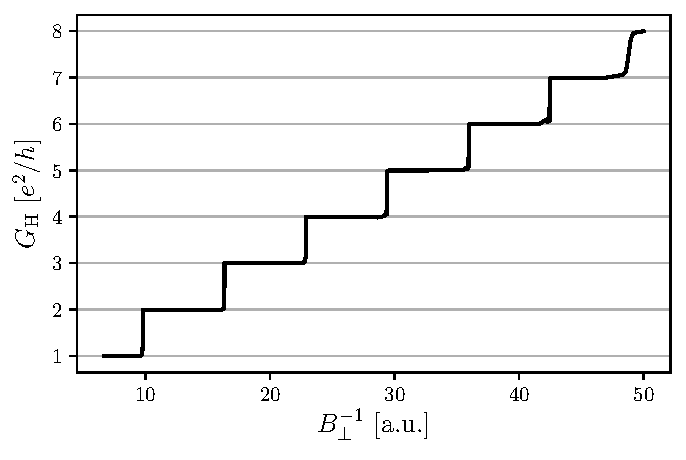
\includegraphics{chapter_introduction/figures/qhe.pdf}
\caption{
The integer quantum Hall effect.
The Hall resistance $R_H$ (reciprocal of the Hall conductance $G_H$) of a two-dimensional electron gas as a function of the perpendicular magnetic field $B_\perp$ at low-temperature.
It displays a stairlike quantized sequence of Hall conductances equal to $ne^2/h$, where $n$ is an integer characterizing each plateau.
\label{fig:qhe_example}}
\end{center}
\end{figure}

\co{More topological states have been realized, one example is TIs.}
The field of topology in condensed matter has substantially grown over the past decades.
Recently, in 2016, the Nobel prize was awarded to Thouless, Haldane, and Kosterlitz for the theoretical findings of topological states.
One of these new states are ``topological insulators,'' which also exhibit edge or surface states and have similarities to the quantum Hall effect, but do not require extreme conditions such as the large magnetic field.
Here, the effect of the magnetic field is replaced by spin-orbit coupling.
This is a coupling between the electron's momentum and spin, effectively causing a momentum dependent magnetic field for electrons that move through a crystal lattice.
The spin-orbit coupling effect is discussed in more detail in Sec.~\ref{sec:hamiltonian_term_by_term}.
Due to the absence of a magnetic field (which breaks time-reversal symmetry in the quantum Hall effect), the edge states always come in counter-propagating pairs, shown in see Fig.~\ref{fig:qhe_example}.

\begin{figure}[!htb]
\begin{center}
% \includegraphics{chapter_introduction/figures/qhe_vs_ti.pdf}
\caption{
Comparison of an insulator, quantum Hall effect, and a topological insulator.
% Rip Fig. 2 and 5 from 10.1103/RevModPhys.82.3045
\label{fig:qhe}}
\end{center}
\end{figure}

\co{Topological states might be used to build a topological quantum computer.}
In addition to the exciting new physical insights into topological materials, topological states might be used to design novel new quantum devices.
One of the most exciting applications is to use these states to build a topological quantum computer by exploiting their non-Abelian properties.
It is predicted that a quantum computer is much faster than a classical computer in performing certain tasks, such as the simulation of quantum systems \cite{Feynman1982} and prime factorization \cite{Shor1994}.
The fundamental building block of the quantum computer is the qubit (or quantum bit), the quantum equivalent of the classical transistor.
Because these qubits store quantum information, they are extremely fragile, and even a small interaction with its environment can destroy its state and result in computational errors.
Physicists experiment with different approaches to create a qubit; for example, there are proposals (and some realizations of) qubits based on quantum optics, ultracold atoms, spin-based systems, and superconducting systems.  % XXX: add refs
In general, one of the most significant problems is to limit and correct the computational errors, and therefore a large fraction of the research is focussed on error-correction \cite{Lidar2013}.
Here, the advantage of using topological states becomes apparent because the topological qubit naturally protects its state against small perturbations in the environment \cite{Nayak2008}.

\co{Majoranas can be used to create this topological quantum computer.}  % XXX: maybe mention that Majoranas are topologically protected
The simplest non-Abelian excitation is the zero-energy Majorana bound state (MBS), which were first proposed to exist as quasiparticle excitations of the $\nu = 5/2$ quantum Hall effect \cite{Read2000,Moore1991}, which requires a high material purity and very low temperatures.
Other early proposals \cite{Gurarie2005,Sarma2006,Tewari2007} rely on rare and exotic $p$-wave superconductors and are extremely challenging to realize experimentally.
In 2008, Fu and Kane suggested a new approach to create MBSs by using a hybrid structure of an ordinary $s$-wave superconductor coupled to a topological insulator to create a state that resembles a spinless $p$-wave superconductor \cite{Fu2008}.
Inspired by this hybrid approach, in 2010, two works \cite{Lutchyn2010,Oreg2010} suggested using a simpler one-dimensional nanowire system coupled to a $s$-wave superconductor.
This simple model combines spin-orbit coupling, superconductivity, electrostatic tunability, and an applied magnetic field.
When tuned into the right parameter regime, this system hosts MBSs at the edges of the nanowire.
Since its introduction, many experiments have detected signatures of MBSs \cite{Mourik2012,Das2012,Deng2012,Deng2016,Deng2016a,Chen2017a}; however, none have demonstrated the presence of MBSs with absolute certainty by showing its non-Abelian statistics.
Because of the simplicity of the model, it can be solved analytically; however, it neglects many physical phenomena that are crucial for understanding the properties of the MBSs.

\co{In this thesis, we study the hybrid Majorana model.}
In this thesis, we study extensions to this model and go beyond the regime that can be studied analytically.
The next sections introduce superconductivity and the topological protection of Majoranas (Sec.~\ref{sec:superconductivity}), non-Abelian statistics (Sec.~\ref{sec:braiding}), the minimal hybrid Majorana model (Sec.~\ref{sec:minimal_majoranas}), and finally, a few extensions to this model (Sec.~\ref{sec:realistic_nanowire}).
At that point, it should be evident that solving this problem requires numerical methods, which is the topic of Sec.~\ref{sec:numerical_methods}.


%%%%%%%%%%%%%%%%%%%%%%%%%%%%%%%%%%%%%%%%%%%%%%%%%%%%%%%%%%%%%%%%%%%%%%%%%%%%%%%%%%%%%%%
%%%%%%%%%%%%%%%%%%%%%%%%%%%%%%%%%% SUPERCONDUCTIVITY %%%%%%%%%%%%%%%%%%%%%%%%%%%%%%%%%%
%%%%%%%%%%%%%%%%%%%%%%%%%%%%%%%%%%%%%%%%%%%%%%%%%%%%%%%%%%%%%%%%%%%%%%%%%%%%%%%%%%%%%%%


\section{Topological protection of Majoranas}\label{sec:superconductivity}
\co{To understand the topological protection of MBS in hybrid structures, we discuss superconductivity.}
This section discusses superconductivity to understand the topological protection of Majorana bound states.
Superconductivity is a phenomenon that occurs in certain materials when cooled below a characteristic critical temperature of $T_{\mathrm{C}}$.
Upon reaching this temperature, the material undergoes a phase transition that results in precisely zero electrical resistance and the expulsion of magnetic fields.
Since the discovery of superconductivity by Heike Kamerlingh Onnes in 1911, considerable efforts have been devoted to finding out how and why it works.
A good understanding of ``conventional'' superconductivity was reached by a pair of important theories: the phenomenological Ginzburg-Landau theory and the microscopic BCS theory.
Today's research focuses on exotic superconductors, high $T_{\mathrm{C}}$ superconductors, and hybrid structures that consist of a superconductor and another material.
In this thesis, we study such hybrid structures.

\subsection{BCS theory and the mean-field approximation}\label{sec:BCS-theory}
\co{We can model superconductivity using BCS theory.}
BCS theory describes superconductivity as a microscopic effect and assumes that two electrons from a Cooper pair where the electrons can effectively attract due to electron-phonon coupling \cite{Cooper1956,Bardeen1957,Bardeen1957a}.
It postulates that superconductivity is caused by a condensation of Cooper pairs at the Fermi energy\footnote{We assume zero temperature $\left(T=0\right)$, so $E_{\textrm{F}}=\mu$, where $\mu$ is the chemical potential.} $E_{\textrm{F}}$ into a boson-like state, a Bose Einstein condensate.
The model Hamiltonian in the language of second quantization ~\cite{Gennes1999} equals:

\begin{equation}
\mathcal{H}_{\textrm{BCS}}=\sum_{\bm{k}\sigma}\epsilon_{\bm{k}}c_{\bm{k}\sigma}^{\dagger}c_{\bm{k}\sigma}+\sum_{\bm{k}\bm{l}}V_{\bm{k}\bm{l}}c_{\bm{k}\uparrow}^{\dagger}c_{-\bm{k}\downarrow}^{\dagger}c_{-\bm{l}\downarrow}c_{\bm{l}\uparrow},\label{eq:BCS}
\end{equation}

where

\begin{tabular}{ll}
$c$            & annihilation operator electron,\tabularnewline
$c^{\dagger}$  & creation operator electron,\tabularnewline
$\epsilon_{k}$ & $E_{k}-\mu$,\tabularnewline
$\mu$          & chemical potential,\tabularnewline
$E_{k}$        & kinetic energy ($\frac{\hbar^{2}k^{2}}{2m}$),\tabularnewline
$m$            & mass,\tabularnewline
$k$            & momentum,\tabularnewline
$\sigma\uparrow,\sigma\downarrow$  & spin of electron,\tabularnewline
$V_{\bm{kl}}$  & interaction potential.\tabularnewline
\end{tabular}

The interaction term includes only the Cooper pairs, which consist of two electrons with opposite spin ($s$-wave symmetry) and opposite momentum that can be denoted as $(\bm{\bm{k}}\uparrow,-\bm{k}\downarrow)$.
Finding the ground state of this so-called pairing Hamiltonian is impossible due to the high degrees of freedom; therefore, we have to make an approximation.  % XXX: check if this is true

\co{We use the mean-field approximation and get the Bogoliubov-de Gennes Hamiltonian and get its spectrum.}
A classic approximation scheme that describes the behavior of conventional superconductors remarkably well is the mean-field approximation.
First we define the quantity
\begin{equation}
b_{\bm{k}}=\left\langle c_{\bm{k}\uparrow}c_{-\bm{k}\downarrow}\right\rangle ,
\end{equation}
which we use to define the so-called gap energy
\begin{equation}
\Delta_{\bm{k}}=-\sum_{\bm{k'}}V_{\bm{kk'}}b_{\bm{k'}}.
\end{equation}
We write the last term in Eq.~\eqref{eq:BCS} as
\begin{equation}
c_{\bm{k}\uparrow}^{\dagger}c_{-\bm{k}\downarrow}^{\dagger}c_{-\bm{l}\downarrow}c_{\bm{l}\uparrow}=\left(c_{\bm{k}\uparrow}^{\dagger}c_{-\bm{k}\downarrow}^{\dagger}-b_{\bm{k}}^{\dagger}+b_{\bm{k}}^{\dagger}\right)\left(c_{-\bm{l}\downarrow}c_{\bm{l}\uparrow}-b_{\bm{l}}+b_{\bm{l}}\right),\label{eq:MF}
\end{equation}
and expand the products.
We neglect the second-order fluctuation term
\begin{equation}
\left(c_{\bm{k}\uparrow}^{\dagger}c_{-\bm{k}\downarrow}^{\dagger}-b_{\bm{k}}^{\dagger}\right)\left(c_{-\bm{l}\downarrow}c_{\bm{l}\uparrow}-b_{\bm{k}}\right)
\end{equation}
in Eq.~\eqref{eq:MF} and rewrite Eq.~\eqref{eq:BCS} to
\begin{equation}
\mathcal{H}_{\textrm{BCS}_{\textrm{MF}}}=\underset{\bm{k},\sigma}{\sum}\epsilon_{\bm{k}}c_{\bm{k}\sigma}^{\dagger}c_{\bm{k}\sigma}-\underset{\bm{k}}{\sum}\left(\Delta_{\bm{k}}c_{\bm{k}\uparrow}^{\dagger}c_{-\bm{k}\downarrow}^{\dagger}+\Delta_{\bm{k}}^{*}c_{-\bm{k}\downarrow}c_{\bm{k}\uparrow}-\Delta_{\bm{k}}b_{\bm{k}}^{*}\right),\label{eq:BCS_MF}
\end{equation}
where the last term is a constant that can be neglected.
We now introduce Nambu spinors
\begin{equation}
\Psi_{\bm{k}}=\left(\begin{array}{c}
c_{\bm{k}\uparrow}\\
c_{-\bm{k}\downarrow}^{\dagger}
\end{array}\right)\label{eq:Nambu}
\end{equation}
and write Eq.~\eqref{eq:BCS_MF} matrix form
\begin{equation}
\mathcal{H}_{\textrm{BCS}_{\textrm{MF}}}=\underset{\bm{k}}{\sum}\Psi_{\bm{k}}^{\dagger}\underset{H_{\textrm{BdG}}}{\underbrace{\left(\begin{array}{cc}
\epsilon_{\bm{k}} & \Delta\\
\Delta_{\bm{k}}^{*} & -\epsilon_{\bm{k}}
\end{array}\right)}}\Psi_{\bm{k}}.
\end{equation}
To calculate the energy spectrum, we can diagonalize the Bogoliubov-de Gennes Hamiltonian $H_{\textrm{BdG}}$ using the unitary Boguliubov transformation matrix $U_{\textrm{B}}$.  % XXX: should I mention this?
Alternatively, we can square $H_{\textrm{BdG}}$ which gives a diagonal matrix
\begin{equation}
H_{\textrm{BdG}}^{2}=\left(\begin{array}{cc}
\epsilon_{\bm{k}}^{2}+\left|\Delta\right|^{2} & 0\\
0 & \epsilon_{\bm{k}}^{2}+\left|\Delta\right|^{2}
\end{array}\right),
\end{equation}
where we can use that the eigenvalues are the square root of the eigenvalues of $H_{\textrm{BdG}}$.
This immediately result in the spectrum
\begin{equation}
E=\pm\sqrt{\epsilon_{\bm{k}}^{2}+\left|\Delta\right|^{2}}.\label{eq:SC_spectrum}
\end{equation}

\co{In the single-particle picture, we essentially double the degrees of freedom and introduce a symmetry.}
The Bogoliubov-de Gennes Hamiltonian acts on the Nambu spinors [Eq.~\eqref{eq:Nambu}] whose first half is composed out of annihilation operators of electrons, and the second half out of creations operators of the same electrons.
To go to a single-particle description (first quantization), we can view the latter creation operators as annihilation operators of an extra set of holes, which doubles the number of degrees of freedom in the system.
Besides the Pauli matrices that act on spin ($\sigma_{i}$ where $i\in x,y,z$) we introduce $\tau_{i}$ to act on the electron-hole degree of freedom.
The Hamiltonian becomes a $4\times4$ matrix\footnote{Here $\otimes$ denotes the Kronecker product and we usually omit $\sigma_{0}$ and $\tau_{0}$.}
\begin{equation}
H_{\textrm{BdG}}=\epsilon_{k}\tau_{z}\otimes\sigma_{0}+\Delta\tau_{x}\otimes\sigma_{0}=\left(\begin{array}{cccc}
\epsilon_{k} & 0 & \Delta & 0\\
0 & \epsilon_{k} & 0 & \Delta\\
\Delta & 0 & -\epsilon_{k} & 0\\
0 & \Delta & 0 & -\epsilon_{k}
\end{array}\right),\label{eq:H_BdG_sc}
\end{equation}
which acts on the wavefunction
\begin{equation}
\Psi=\left(\psi_{\textrm{e}\uparrow},\psi_{\textrm{e}\downarrow},\psi_{\textrm{h}\downarrow},-\psi_{\textrm{h}\uparrow}\right)^{T},\label{eq:4wf}
\end{equation}
where $\psi_{\textrm{e}}$, $\psi_{\textrm{h}}$ are the electron and hole components of the wave function, and $\psi_{\uparrow}$, $\psi_{\downarrow}$ are the spin-up and spin-down states.
Because the holes are related to the electrons, $H_{\textrm{BdG}}$ has a particle-hole symmetry, and it determines the material's specific topology.
Symmetry and its resulting topology is the topic of the next section, after which, we will discuss this particle-hole symmetry.

\subsection{Topology and symmetry}\label{sec:topology}
\co{Symmetry determines a system's topology.}
Symmetry plays a fundamental part in physics.
In condensed matter systems, only three discrete symmetries are important: time-reversal symmetry $\mathcal{T}$, particle-hole symmetry $\mathcal{P}$, and chiral symmetry $\mathcal{C}$.
Wigner's theorem states that a symmetry must either be a unitary or an anti-unitary operator.
Both $\mathcal{T}$ and $\mathcal{P}$ have anti-unitary operators and may square either to $+1$ or $-1$ depending on the specifics of the system.
Chiral symmetries have a unitary operator and always squares to $+1$.
The combination of these three symmetries from ten symmetry classes~\cite{Altland1997}.
Each class is characterized by the absence or presence of these symmetries, and together with the dimensionality of a sytem determines the specific topological invariant it has.
Topology studies whether objects can be continuously transformed into each other.
The object that is studied in condensed matter is the Hamiltonian of a system.
If two Hamiltonians can be continuously transformed\footnote{An example of a continuous transformation from $H_{1}$ to $H_{2}$: $H=\alpha H_{1}+(1-\alpha)H_{2}$ where $\alpha=0\rightarrow1$.} into each other without changing the topological invariant: the systems are said to be topologically equivalent.
How a topological invariant changes, varies for the different symmetry classes.

\co{The PHS relates electrons to holes and this is obvious in its spectrum.}
We ended Sec.~\ref{sec:BCS-theory} by noting that $H_{\textrm{BdG}}$ [Eq.~\eqref{eq:H_BdG_sc}] has a particle-hole symmetry $\mathcal{P}$.
This Hamiltonian acts on a two-component wave function $\psi_{\textrm{BdG}}=\left(u,v\right)^{T}$ with $u$ electron component and $v$ the hole component.
The symmetry of this Hamiltonian is most obvious in its dispersion relation, where each eigenstate $\psi_{E}=\left(u_{0},v_{0}\right)^{T}$ has a particle-hole symmetric partner at $\psi_{-E}=\left(\mathcal{P}u_{0},\mathcal{P}v_{0}\right)^{T}$.
In constructing $H_{\textrm{BdG}}$, we artificially doubled the degrees of freedom by considering electrons and holes separately.
Therefore, the creation operator $c^{\dagger}$ of the quasiparticle in the $\psi_{E}$ state is equal to the annihilation operator $c$ of the quasiparticle in the $\psi_{-E}$ state.
From this, it is clear that $\psi_{E}$ and $\psi_{-E}$ correspond to the same quasiparticle, and the creation of a quasiparticle with positive energy is identical to the annihilation of a quasiparticle with negative energy.
In a one or higher dimensional system, the operator $\mathcal{P}$ will not only send $E \rightarrow -E$ but will also send the momentum $k \rightarrow -k$ as
\begin{equation}
\mathcal{P^{\dagger}}H\left(k\right)\mathcal{P}=-H\left(-k\right).
\end{equation}

\co{At E=0, we get a the Majorana condition.}
At zero energy, something curious happens: here we have a state $\psi_{0}$ that upon applying $\mathcal{P}$ is transforms into itself $\mathcal{P}\psi_{0}=\psi_{0}$.
This state has a creation operator $\gamma^{\dagger}$ that is identical to the annihilation operator $\gamma$ of itself, so $\gamma^{\dagger}=\gamma$.
We call this property the Majorana condition.
If we use the Majorana condition in the fermionic commutation relation
\begin{equation}
\gamma^{\dagger}\gamma+\gamma\gamma^{\dagger}=1
\end{equation}
we get $\gamma^{\dagger}\gamma=1/2$ and see that the Majorana state is always half occupied.
Removing a Majorana from zero energy is, therefore, only possible if it is paired with another Majorana to form a fermionic mode.
Later, in Sec.~\ref{sec:braiding} we make use of this property and show how these Majoranas exhibit non-Abelian statistics.
Subsequently, in Sec.~\ref{sec:minimal_majoranas}, we show that it is possible to create Majoranas at two opposite edges of a nanowire where they do not couple and are pinned to $E=0$; this provides the so-called topological protection.
Here, the fermionic mode (which is occupied or unoccupied,) is the quantity that is protected.

\co{Having a PHS means symmetry class D, which in 1D has a Z2 invariant that indicates the presence or absence of Majoranas.}
The symmetry class of the one-dimensional system we study in this thesis has a particle-hole symmetry $\mathcal{P}$, and therefore belongs to class $\mathcal{D}$.
This class has a $\mathcal{Z}_2$ topological invariant $Q$ that is the sign of the Pfaffian of the Hamiltonian: $Q=\sgn\Pf\left(H\right)$.
This invariant can only assume two values ($+1$ or $-1$) and indicates the presence or absence of Majoranas.
\footnote{The Pfaffian for an anti-symmetric matrix is related to the determinant as $\Pf(A)^{2}=\det(A)$.}
This topological invariant is only defined for a system with an energy gap, which means the Hamiltonian of the system has no eigenvalues in a finite interval around zero energy, as in Eq.~\ref{eq:H_BdG_sc}.
If we can continuously transform a Hamiltonian $H_{1}$ into another Hamiltonian $H_{2}$ without ever closing the energy gap, we say $H_{1}$ and $H_{2}$ are topologically equivalent, and thus have the same topological invariant.


%%%%%%%%%%%%%%%%%%%%%%%%%%%%%%%%%%%%%%%%%%%%%%%%%%%%%%%%%%%%%%%%%%%%%%%%%%%%%%%%%%%%%%%
%%%%%%%%%%%%%%%%%%%%%%%%%%%%%%%%%%%%%% BRAIDING %%%%%%%%%%%%%%%%%%%%%%%%%%%%%%%%%%%%%%%
%%%%%%%%%%%%%%%%%%%%%%%%%%%%%%%%%%%%%%%%%%%%%%%%%%%%%%%%%%%%%%%%%%%%%%%%%%%%%%%%%%%%%%%


\section{Non-Abelian statistics and braiding}\label{sec:braiding}
\co{Majoranas have non-Abelian statistics which is the motivation to study them.}
For many researchers, the ultimate motivation to study Majoranas is the fact that they have a fascinating property, non-Abelian quantum statistics.
Quantum statistic studies what happens to wavefunctions describing identical particles when their positions are exchanged in space.
In introductory quantum mechanics courses, we learned that particles are divided into two classes according to quantum statistics: bosons which stay the same under the exchange and fermions for which the wavefunction changes sign.
However, Majorana bound states do not belong to either of these and are non-Abelian anyons.
The operation of exchanging two Majoranas (called braiding) can send the system into a different state with the same particle configuration.
Explaining how one could experimentally perform a braiding operation is beyond the scope of this thesis; therefore, we will focus on the mathematical operations that describe the braiding process.

\co{Multiple Majoranas form a ground state manifold.}
Exchanging two Majoranas in 1D is ill-defined because it is impossible to swap them without having them collide, which would annihilate them.
We can construct a network of nanowires to form T-junctions (see Fig.~\ref{fig:Majorana-T-junction}), which allows us to exchange positions of Majoranas.
Here, one can temporarily move a Majorana to one of the unoccupied wires and perform the exchange without the Majoranas ever becoming too close to each other.
\begin{figure}
\begin{center}
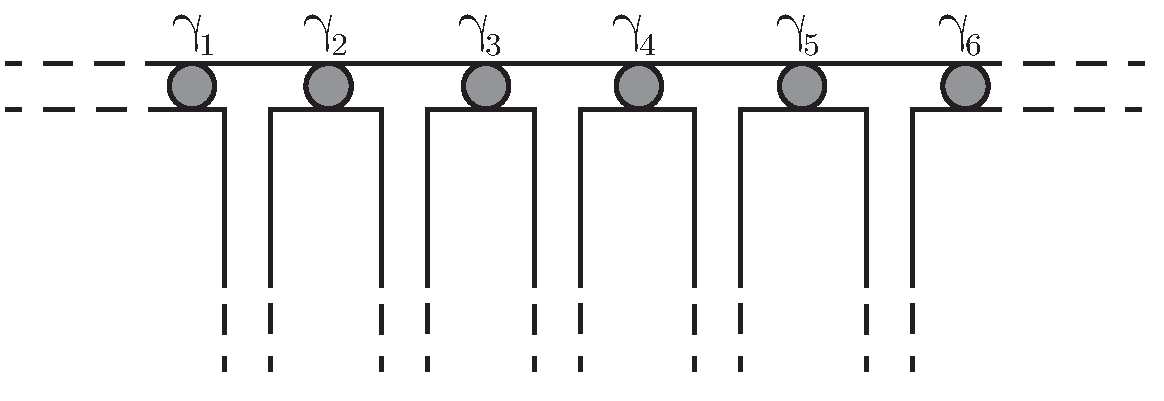
\includegraphics[width=0.95\textwidth]{chapter_introduction/figures/T-junction-network.pdf}
\centering{}
\caption{Majorana T-junction.
The circles represent the Majoranas $\gamma_{1}...\gamma_{6}$.
This network of nanowires allows for the exchange of two Majoranas without having them collide.
This is possible by temporarily bringing a Majorana to one of the
vertical wires and then swapping the position of the other Majorana.
\label{fig:Majorana-T-junction}}
\end{center}
\end{figure}
The only thing that distinguishes Majoranas is their position in the network.
That means that if we exchanged two Majoranas in space, the system would look exactly the same as it looked before the exchange.
We now assume the energy spectrum is gapped for $|E|<\Delta$ with the Majorana ground state at $E=0$.
If this ground state contains several Majoranas, there will be several states all at zero energy, forming a  ``ground state manifold.''

\co{We consider $N$ Majoranas and write down its state of fermionic modes.}
From now on, we only consider the states corresponding to the Majoranas and neglect the states that live in the bulk ($E \geq \Delta$).
As mentioned in Sec.\ref{sec:topology}, a Majorana only has half a degree of freedom, and thus, they can only be assigned quantum states in pairs.
In Fig.~\ref{fig:Majorana-T-junction} we see six Majoranas (3 pairs), but for generality lets consider $N$ pairs.
By pairing two Majoranas (two times half a degree of freedom), we can form fermionic modes that will give us two possible degenerate quantum states, either unoccupied $\ket 0$ or occupied $\ket 1$.
By pairing up neighboring Majoranas $\gamma_{2n-1}$ and $\gamma_{2n}$ we get a creation operator that is its own complex conjugate $c_{n}^{\dagger}=\tfrac{1}{2}(\gamma_{2n-1}+i\gamma_{2n})$, where $c$ is a fermionic creation operator.
Each pair gives two possible quantum states, so $N$ pairs will have $2^{N}$ possible states.
We can represent every such state with a ket
\begin{equation}
\left|s_{1},s_{2},\dots,s_{N}\right\rangle,
\end{equation}
where $s_{n}$ is either unoccupied $0$ or occupied $1$.
These states form a complete basis of the Hilbert space of the set of Majoranas.

\co{The parity of the groundstate is an observable.}
We define the fermion parity operator
\begin{equation}
P_{n}\equiv1-2c_{n}^{\dagger}c_{n}=i\gamma_{2n-1}\gamma_{2n},
\end{equation}
that acts on the states and where we recognize the $c_{n}^{\dagger}c_{n}$ term as the number operator.
All basis states in the Hilbert space of Majoranas are eigenstates of $P_{n}$.
For example, we have
\begin{subequations}
\begin{equation}
P_{1}\left|0,\dots\right\rangle \ =(1-2c_{1}^{\dagger}c_{1})\left|0,\dots\right\rangle =+\left|0,\dots\right\rangle ,
\end{equation}

\begin{equation}
P_{1}\left|1,\dots\right\rangle \ =(1-2c_{1}^{\dagger}c_{1})\left|1,\dots\right\rangle =-\left|1,\dots\right\rangle .
\end{equation}
\end{subequations}
Another essential property of Majoranas is that a pair of Majorana operators all anti-commute with each other.
So
\begin{equation}
(\gamma_{1}\gamma_{2})(\gamma_{3}\gamma_{4})=(\gamma_{3}\gamma_{4})(\gamma_{1}\gamma_{2}),
\end{equation}
but when the pairs share a Majorana they do not commute anymore
\begin{equation}
(\gamma_{1}\gamma_{2})(\gamma_{2}\gamma_{3})=-(\gamma_{2}\gamma_{3})(\gamma_{1}\gamma_{2}).
\end{equation}
In Sec.~\ref{sec:superconductivity}, we introduced the Hamiltonian Eq.~\eqref{eq:H_BdG_sc}, which does not conserve particle number; however, the parity is conserved.
The total parity can be obtained by multiplying all parity operators
\begin{equation}
P_{\textrm{tot}}=P_{1}\cdot P_{2}\cdot\,\dots\,\cdot P_{N}=i^{N}\gamma_{1}\gamma_{2}\dots\gamma_{2N}.
\end{equation}
where $P_{\textrm{tot}}$ has eigenvalues $\pm1$.
The parity is an observable and can, therefore, be experimentally measured.

\co{We can deduce the braiding operator that exchanges two Majoranas.}
We can now start to think about what would happen when we exchange two Majoranas~\cite{Ivanov2001}.
Our ground state manifold $\ket\Psi$ will never leave the ground state if we perform the exchange slowly enough.
The exchange of two Majoranas $\gamma_{n}$ and $\gamma_{m}$ will change the ground state $\left|\Psi\right\rangle \to U\left|\Psi\right\rangle $ where $U$ is a unitary operator.
The exact form of $U$ can be derived without a direct calculation.
We do this by assuming that $U$ only depends on the Majoranas involved in the exchange ( $\gamma_{n}$ and $\gamma_{m}$) and by using that the slow exchange does not change the parity of the system because the system stays gapped at all times.
Since the parity is conserved we know: $U$ commutes with the total fermion parity $[U,P_{\textrm{tot}}]=0$, and that $U$ can only depend on the product $i\gamma_{n}\gamma_{m}$.
This product is Hermitian, so we can create a unitary operator by taking the exponential of $i$ times this Hermitian operator as
\begin{equation}
U\equiv\exp(\beta\gamma_{n}\gamma_{m})=\cos(\beta)+\gamma_{n}\gamma_{m}\sin(\beta),
\end{equation}
where $\beta$ is a real coefficient to be determined.
In the last equality we used $(\gamma_{n}\gamma_{m})^{2}=\gamma_{n}\gamma_{m}\gamma_{n}\gamma_{m}=-\gamma_{n}\underset{=1}{\underbrace{\gamma_{m}\gamma_{m}}}\gamma_{n}=-1$
in the Taylor expansion.
We now move to the Heisenberg picture where we look at the evolution of the Majorana operators in time
\begin{subequations}
\begin{equation}
\gamma_{n}\to U\gamma_{n}U^{\dagger}=\left(\cos\beta+\gamma_{n}\gamma_{m}\sin\beta\right)\gamma_{n}\left(\cos\beta+\gamma_{m}^{\dagger}\gamma_{n}^{\dagger}\sin\beta\right)
\end{equation}

\begin{equation}
=\gamma_{n}\cos^{2}\beta+\left(\gamma_{n}\gamma_{m}^{\dagger}\gamma_{n}^{\dagger}+\gamma_{n}\gamma_{m}\gamma_{n}\right)\sin\beta\cos\beta+\gamma_{n}\gamma_{m}\gamma_{n}\gamma_{m}^{\dagger}\gamma_{n}^{\dagger}\sin^{2}\beta
\end{equation}

\begin{equation}
=\gamma_{n}\cos^{2}\beta-\gamma_{n}^{\dagger}\sin^{2}\beta-2\gamma_{m}\sin\beta\cos\beta
\end{equation}

\begin{equation}
=\gamma_{n}\cos2\beta-\gamma_{m}\sin2\beta
\end{equation}
\end{subequations}
Similarly we get
\begin{equation}
\gamma_{m}\to U\gamma_{m}U^{\dagger}=\gamma_{m}\cos2\beta+\gamma_{n}\sin2\beta.
\end{equation}
After the exchange happened we know that $\gamma_{m}\to\gamma_{n}$ and $\gamma_{n}\to\gamma_{m}$, this leads to $\beta=\pm\pi/4$.
The two signs make sense; this distinguishes the clockwise and the counterclockwise exchange of the Majoranas.
We now found an operator that exchanges two Majoranas
\begin{equation}
U=\exp\left(\pm\frac{\pi}{4}\gamma_{n}\gamma_{m}\right)=\tfrac{1}{\sqrt{2}}\left(1\pm\gamma_{n}\gamma_{m}\right).\label{eq:U_nm}
\end{equation}

\co{As an example, we apply this operator to the simplest non-trivial case of having just four Majoranas.}
As an example, lets now look at what happens when we have just four Majoranas $\gamma_{1}$, $\gamma_{2}$, $\gamma_{3}$, and $\gamma_{4}$.
The four basis states in the ground state manifold are
\begin{equation}
\left|00\right\rangle ,\left|01\right\rangle ,\left|10\right\rangle ,\left|11\right\rangle ,\label{eq:basis}
\end{equation}
where the first number is the occupation number of the fermionic mode $c_{1}^{\dagger}=\tfrac{1}{2}(\gamma_{1}+i\gamma_{2})$ and the second number the occupation number of $c_{2}^{\dagger}=\tfrac{1}{2}(\gamma_{3}+i\gamma_{4})$.
For instance, if we start from the state $\left|00\right\rangle $ and we exchange $\gamma_{2}$ and $\gamma_{3}$ by applying $U_{23}=\tfrac{1}{\sqrt{2}}\left(1\pm\gamma_{2}\gamma_{3}\right)$, we obtain\footnote{See appendix \ref{chap:U_der} for derivations of $U_{nm}$.}  % XXX: add this to the appendix.
\begin{equation}
\left|00\right\rangle \to U_{23}\left|00\right\rangle =\tfrac{1}{\sqrt{2}}\left(\left|00\right\rangle +i\left|11\right\rangle \right).
\end{equation}
Here we see a superposition of states, which is not like bosons or fermions at all, where the exchange can only change the sign.
This property makes Majoranas non-Abelian anyons, and the exchange of two non-Abelian anyons is usually called braiding.
Using these braiding operations, we can create a qubit that can perform a certain set (but not all) of rotations on the single-qubit Bloch sphere.
This means that some of the qubit operations are topologically protected, which reduces the amount of error-correction needed in comparison with a non-topological qubit, and in turn, means that fewer physical qubits are required.


%%%%%%%%%%%%%%%%%%%%%%%%%%%%%%%%%%%%%%%%%%%%%%%%%%%%%%%%%%%%%%%%%%%%%%%%%%%%%%%%%%%%%%%
%%%%%%%%%%%%%%%%%%%%%%%%%%% MAJORANAS IN A MINIMAL NANOWIRE %%%%%%%%%%%%%%%%%%%%%%%%%%%
%%%%%%%%%%%%%%%%%%%%%%%%%%%%%%%%%%%%%%%%%%%%%%%%%%%%%%%%%%%%%%%%%%%%%%%%%%%%%%%%%%%%%%%


\section{Majoranas in a minimal hybrid nanowire}\label{sec:minimal_majoranas}
\co{Superconductivity, spin-orbit coupling, a Zeeman field, and tuned µ leads to the appearance of Majoranas near the edges of the wire.}
The combined effect of superconductivity, spin-orbit coupling, and a Zeeman field can lead to the appearance of Majoranas near the edges of the wire~\cite{Lutchyn2010,Oreg2010}.
To understand how this happens, we study the effects of the various terms in the Hamiltonian.
As discussed in Sec.~\ref{sec:topology}, the appearance of Majoranas is a topological effect and is accompanied by the change of the topological invariant $Q$ of symmetry class $\mathcal{D}$.
This invariant can only assume $Q=+1$ (no Majoranas) and $Q=-1$ (Majoranas present) and changes when the band gap closes and reopens.

\begin{figure}
\begin{center}
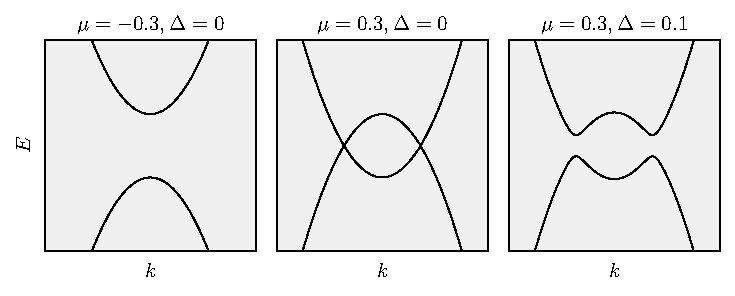
\includegraphics[width=0.95\textwidth]{chapter_introduction/figures/triv_topo_bandstructure.pdf}
\caption{Band structures of Hamiltonians with chemical potential $\mu=-0.3$ and superconducting gap $\Delta=0$ (left); $\mu=0.3$ and $\Delta=0$ (middle); and $\mu=0.3$ and $\Delta=0.1$ (right).
\label{fig:triv_topo_bandstructure}}
\end{center}
\end{figure}

\subsection{The Hamiltonian: term by term}\label{sec:hamiltonian_term_by_term}
\co{We show what the effect of these individual terms is on the band structure.}
The complete model Hamiltonian is rather complicated; therefore, we start with a one-dimensional single band Hamiltonian and study its band structure while adding the terms needed to make a topological band structure and ``engineer'' our way towards Majoranas.
The Hamiltonian in its simplest form is quadratic in momentum and has an off-set in chemical potential $\mu$
\begin{equation}
H=\left(\frac{\bm{p}^{2}}{2m}-\mu\right)\tau_{z},\label{eq:simple_ham}
\end{equation}
where $\tau_{z}$ is a Pauli matrix that acts on the electron-hole substructure.
The band structure for this Hamiltonian with $\mu=-0.3$ is shown in Fig.~\ref{fig:triv_topo_bandstructure} (left).
We assume that this band structure is topologically trivial and has $Q=+1$.
Because this Hamiltonian acts trivially in spin-space, the bands in Fig.~\ref{fig:triv_topo_bandstructure} (left) are doubly degenerate.
Finally, the electrons are at positive energy $E$ and the holes on $-E$.

\co{We require a band gap, so we add superconductivity, resulting in a BdG Hamiltonian with a gapped spectrum.}
Next, we raise $\mu$, which shifts the bands [see Fig.~\ref{fig:triv_topo_bandstructure} (middle)].
In Sec.~\ref{sec:topology}, we explained that the topological invariant is only defined for a system with an energy gap.
This band structure has no band gap, and therefore cannot be topological.
Further, in Sec.~\ref{sec:superconductivity} we observed that a BdG Hamiltonian has a gapped spectrum [Eq.~\eqref{eq:SC_spectrum}], so we add $\Delta\tau_{x}$, which results in
\begin{equation}
H_{\textrm{BdG}}=\left(\frac{\bm{p}^{2}}{2m}-\mu\right)\tau_{z}+\Delta\tau_{x},
\end{equation}
and opens a gap because $\tau_{x}$ mixes the electron and holes [see Fig.~\ref{fig:triv_topo_bandstructure} (right)].

\co{We break the spin degeneracy using a magnetic field.}
We are left with a gapped spectrum; however, we closed the band gap twice because of the doubly degenerate spin bands both crossing zero energy simultaneously.
The spin degeneracy (called a Kramers degeneracy\footnote{A Kramers degeneracy would result in two Majoranas per edge (just a fermion).}) is a result of a time-reversal symmetry and needs to be broken to create isolated Majoranas.
To couple to spin we introduce the Zeeman field $E_\textrm{Z}\sigma_{x}=\frac{1}{2}g\mu_{\textrm{B}}B\sigma_{x}$ in the Hamiltonian
\begin{equation}
H_{\textrm{BdG}}=\left(\frac{\bm{p}^{2}}{2m}-\mu\right)\tau_{z}+\Delta\tau_{x}+\frac{1}{2}g\mu_{\textrm{B}}B\sigma_{x},\label{eq:zeeman}
\end{equation}
where $g$ is the Landé factor, $\mu_{\textrm{B}}$ the Bohr magneton, and $B$ magnetic field along $x$, parallel to the wire direction.
In Fig.~\ref{fig:zeeman} we plot the effect of a magnetic field on the band structure and observe that a magnetic field breaks the Kramers degeneracy.
\begin{figure}
\begin{center}
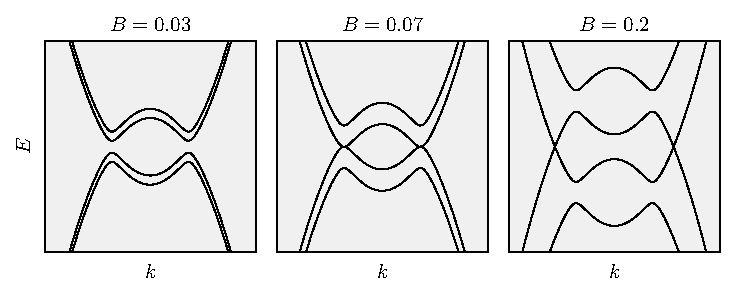
\includegraphics[width=0.95\textwidth]{chapter_introduction/figures/zeeman.pdf}
\caption{Band structures of Eq.~\eqref{eq:zeeman} for different values of magnetic field and $\Delta=0.1$, $\mu=0.3$.
\label{fig:zeeman}}
\end{center}
\end{figure}
The bands moving towards each other have opposite spin (orthogonal states), and as we see in Fig.~\ref{fig:zeeman} (middle and left), these spins do not couple.
The problem is that Zeeman conserves spin in $x$-direction, and therefore spin is still a good quantum number.
We know that Majoranas must be spinless because they are their own complex conjugate.

\co{To break spin-rotation symmetry, we introduce the spin-orbit coupling, which by itself is not enough to create Majoranas.}
The solution to this last problem is spin-orbit coupling, which in its simplest form is Rashba: $H_{\textrm{Rashba}}=-\alpha p_{x}\sigma_{y}\tau_{z}$.
The Hamiltonian is now complete and equals
\begin{equation}
H_{\textrm{BdG}}=\left(\frac{\bm{p}^{2}}{2m}-\mu\right)\tau_{z}+\Delta\tau_{x}+\frac{1}{2}g\mu_{\textrm{B}}B\sigma_{x}-\alpha p_{x}\sigma_{y}\tau_{z}.\label{eq:rashba}
\end{equation}
Spin-orbit by itself---eventhough it couples spin---is insufficient to break the Kramers degeneracy.
In Fig.~\ref{fig:SO_no_zeeman}, we see that raising $\alpha$ moves the different spin bands away in either $+k$ or $-k$ direction.
However, a degeneracy remains at $k=0$, revealing why a magnetic field is needed.
\begin{figure}
\begin{center}
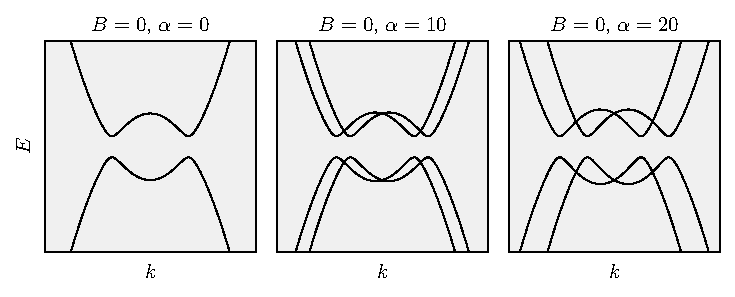
\includegraphics[width=0.95\textwidth]{chapter_introduction/figures/SO_no_zeeman.pdf}
\caption{Band structures of Eq.~\eqref{eq:rashba} for different values of spin-orbit coupling $\alpha$ and $B=0$, $\Delta=0.1$, $\mu=0.3$.
\label{fig:SO_no_zeeman}}
\end{center}
\end{figure}
Including a magnetic field opens the gap at $k=0$ (see Fig.~\ref{fig:SO_and_zeeman}) making the system topologically nontrivial.
If the system is of a finite length, it will host Majoranas on its edges at $E=0$.
\begin{figure}
\begin{center}
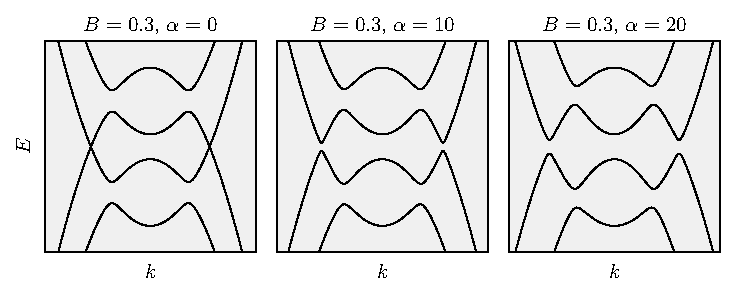
\includegraphics[width=0.95\textwidth]{chapter_introduction/figures/SO_and_zeeman.pdf}
\caption{Band structures of Eq.~\eqref{eq:rashba} for different values of spin-orbit coupling $\alpha$ and $B=0.3$, $\Delta=0.1$, $\mu=0.3$.
\label{fig:SO_and_zeeman}}
\end{center}
\end{figure}

\subsection{Wavefunction}
\co{Using the right parameters, we can plot the Majorana wavefunction.}
We now have all the terms in the Hamiltonian to create a topological band structure, which we calculate for an infinite system (i.e., system with a translational symmetry).
To observe Majoranas, we need to diagonalize the Hamiltonian of a finite system with the same parameters that resulted in the topological band structure and plot the wavefunction with the lowest energy: the Majorana wavefunction.
In Fig.~\ref{fig:wavefunction_1d} (left), we plot the probability density of the Majorana wavefunction and observe that it is indeed localized near edges of the nanowire.
This wavefunction decays exponentially from both sides with a decay length $\xi_\textrm{M}$.

\begin{figure}
\begin{center}
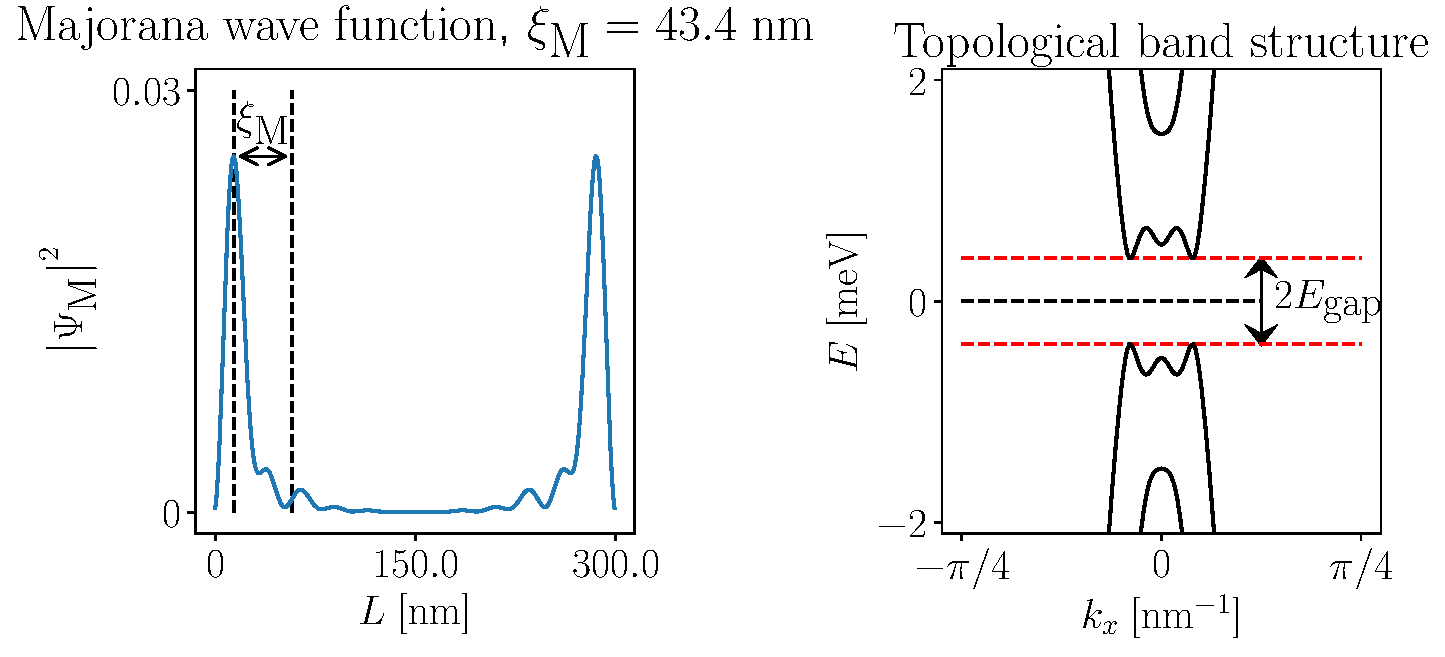
\includegraphics[width=0.95\textwidth]{chapter_introduction/figures/wf_and_band_structure.pdf}
\caption{Probability density and band structure of a 1D system.
The probability density of the lowest energy wavefunction (Majorana wavefunction) of a \SI{0.3}{\micro\metre} long nanowire (left) and a topological band structure (right) with the same parameter values, but for an infinite system.
The Majorana length $\xi$---the decay length of the wavefunction---in the left plot is $\xi_\textrm{M}=\SI{43.4}{nm}$.
\label{fig:wavefunction_1d}}
\end{center}
\end{figure}

\subsection{Phase diagram}
\co{With a phase diagram, we show for which tunable parameters the system is topological.}
The Hamiltonian [Eq.~\eqref{eq:rashba}] contains a few fundamental constants and constants that are material dependent; however, the chemical potential $\mu$ and magnetic field $B$ can be adjusted in an experiment.
A good question is, for which values of $B$ and $\mu$ the system is topological.
Due to its compactness, this model can be solved analytically, and it predicts that Majorana bound states appear when $E_\textrm{Z}^{2}>\mu^{2}+\Delta^{2}$, when the Zeeman energy becomes larger than the harmonic mean of the superconducting gap and the chemical potential.
In Fig.~\ref{fig:phase_diagram_1D} we plot a phase diagram, which indicates for which value of $\left(B,\; \mu\right)$ the system is topological.
In the next section, we will extend this model to three dimensions and study how it modifies the phase diagram.

\begin{figure}
\begin{center}
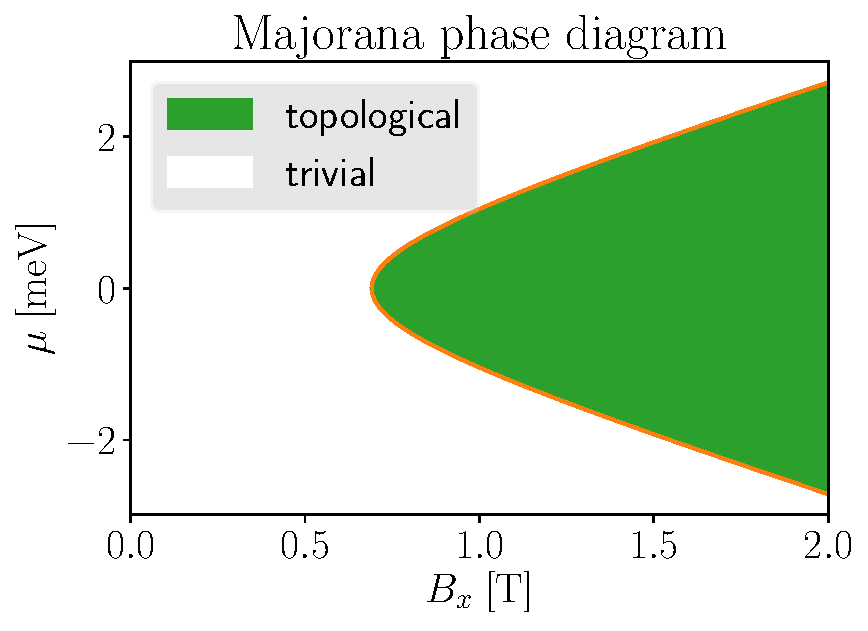
\includegraphics[width=0.7\textwidth]{chapter_introduction/figures/phase_diagram_1D.pdf}
\caption{A phase diagram of a one-dimensional Majorana nanowire device as a function of magnetic field $B$ and chemical potential $\mu$.
The color indicates whether the system is in the topological or trivial phase.
This system becomes topological whenever $E_\textrm{Z}^{2}>\mu^{2}+\Delta^{2}$.
\label{fig:phase_diagram_1D}}
\end{center}
\end{figure}


%%%%%%%%%%%%%%%%%%%%%%%%%%%%%%%%%%%%%%%%%%%%%%%%%%%%%%%%%%%%%%%%%%%%%%%%%%%%%%%%%%%%%%%
%%%%%%%%%%%%%%%%%%%%%%%%% MAJORANAS IN A REALISTIC 3D NANOWIRE %%%%%%%%%%%%%%%%%%%%%%%%
%%%%%%%%%%%%%%%%%%%%%%%%%%%%%%%%%%%%%%%%%%%%%%%%%%%%%%%%%%%%%%%%%%%%%%%%%%%%%%%%%%%%%%%


\section{Majoranas in a more realistic 3D hybrid nanowire}\label{sec:realistic_nanowire}
\co{The simple model is great, but experiments does not agree, so we need to include more physical effects.}
The simple one-dimensional model we introduced in the previous section is useful because it can be solved analytically and therefore, it gives us many insights.
However, because of its simplicity, it also ignores multiple relevant physical effects.
For example, the model assumes a one-dimensional nanowire even though we live in a three-dimensional world, and so does the nanowire device when an experimentalist creates it.
Besides the additional orbitals that are present in a three-dimensional system, the magnetic flux penetrating the nanowire cross-section modifies the Hamiltonian and changes the complex phases of the moving quasiparticles.
Further, the simple model assumes a tunable but constant chemical potential $\mu$ inside the nanowire.
In an experiment, the nanowire is close to a metal gate at a certain voltage; its electric field changes the potential inside the nanowire non-homogeneously.
In addition to these theoretical considerations, the experimental measurement results do not correspond to the predictions that the simple model makes.
For example, for measuring the conductance from a nanowire hosting Majoranas to a normal lead, the model predicts a quantized conductance of $2 e^2/h$ at a bias voltage of $V_\textrm{B}=0$, the so-called zero-bias peak.
Nearly all experiments \footnote{not arXiv:1710.10701} that measure this fail to reproduce this zero-bias peak where the conductance is quantized.
Another effect that is not captured by the simple model is the superconducting density of states (DOS), which in theory predicts a vanishing DOS inside the gap ($|E|<\Delta$) but the experiment a non-zero DOS persists, this phenomenon is also called ``soft gap.''
Because of these limitations, we will improve the simple model by adding relevant physical effects.

\co{In 3D more orbitals are present, breaking the simple E_z²>µ²+Δ² requirement for Majoranas.}
In 3D, the model Hamiltonian [Eq.~\eqref{eq:rashba}] is modified to
\begin{equation}
H_{\textrm{BdG}}=\left(\frac{\bm{p}^{2}}{2m}-\mu\right)\tau_{z}+\Delta\tau_{x}+\frac{1}{2}g\mu_{\textrm{B}}B\sigma_{x}+\alpha\left(p_{y}\sigma_{x}-p_{x}\sigma_{y}\right)\tau_{z},\label{eq:3D_Ham}
\end{equation}
such that it includes the transverse part of the Rashba spin-orbit.
The two additional dimensions result in more orbitals and equivalently more bands; therefore, the condition $E_\textrm{Z}^{2}>\mu^{2}+\Delta^{2}$ for a topological nanowire is no longer valid.
Because there are more bands, multiple Majoranas can be created on both edges of the nanowire as $\mu$ increases.
However, these additional Majoranas are not topologically protected (without an additional symmetry), and a small perturbation can pair-wise annihilate all but $N \mod 2$ of them.
The position of the phase boundaries now also depends on the cross-section's geometry.
For example, Fig.~\ref{fig:topo_bands} shows a phase diagram (and band structures at different combinations of $B$ and $\mu$) of a nanowire with a cylindrical cross-section.
\begin{figure}
\begin{center}
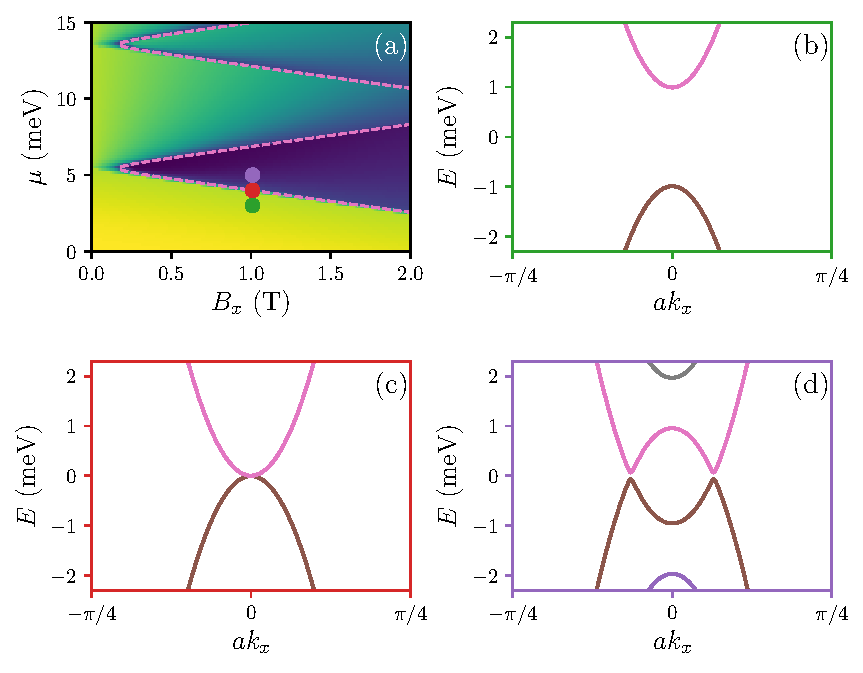
\includegraphics[width=0.8\textwidth]{chapter_introduction/figures/phase_diagram_with_bands.pdf}
\caption{Topological phase diagram (a) of a 3D system where the dot indicate the parameter values of $B,\; \mu$ at which the surrounding band structures (b-d) are plotted.
The color in the phase diagram (a) shows the size of the topological gap and the dashed lines are the topological phase boundaries.
The band structure (b) is trivial but near a phase transition, (c) is at the phase transition, and (d) is inside of the topological regime.
\label{fig:topo_bands}}
\end{center}
\end{figure}

\co{Whenever a magnetic flux can penatrate the nanowire, the canonical momentum operator is modified to include the vector potential.}
Whenever a magnetic flux can penatrate a surface of the nanowire, the canonical momentum operator in Eq.~\eqref{eq:3D_Ham} is modified to include the vector potential
\begin{equation}
\bm{p} \rightarrow -i \hbar \nabla + e \bm{A} \tau_z,
\end{equation}
where $e$ is the electron charge.
In the weak coupling regime---with a non transparent semiconductor/superconductor interface---and a wire that is symmetric with respect to the wire axis, the vector potential is $\mathbf{A}={\left[ B_y (z - z_0) - B_z (y - y_0), 0, B_x (y - y_0)\right]}^{T}$, which is chosen such that it does not depend on $x$.
Here, we set the offsets $y_0$ and $z_0$ such that the average vector potential vanishes in the superconductor.
Physically, this choice corresponds to a limit where the total supercurrent $J_s$ is zero, appropriate for existing devices that use NbTiN as a superconducting shell.
In this case, the superconductor can be considered as a perturbation that only provides the electron-hole coupling in the normal regime.
However, devices that have a thin Al shell are in the strong coupling regime.
Because of the high density inside the superconductor (compared to the semiconductor), the wire can no longer be considered as symmetric with respect to the wire axis.
To get correct physical observables from both the vector potential and the superconducting phase difference~\cite{Wojcik2018}, we have to ensure that the total supercurrent cancels out,
\begin{equation}
j_s = \frac{1}{2}\nabla \Phi - e \bm{A}=0.  % XXX: check units, from Georg's paper Eq. (9).
\end{equation}
At zero temperature, this can be archived by minimizing the kinetic energy, which is proportional to $E_s \propto \int d \bm{x} J_s^2(\bm{x})$ ~\cite{Winkler2019}.
This minimization results in the correct vector potential and the superconducting phase.
The inclusion of the orbital effect modifies the phase diagram shown in Fig.~\ref{fig:topo_bands}.
Chapter ~\ref{ch:orbitalfield} discusses the weakly coupled superconductor case while Ch.~\ref{ch:shortjunction} discusses the strongly coupled superconductor case.

\co{A real system's material is not perfectly smooth and has impurities, and we can model this disorder by random onsite energy.}
Perfectly ordered crystalline solids are characterized by a faultlessly regular arrangement of their atoms in a crystal lattice, yet, these do not occur in nature~\cite{Nolting1970}.
Real solid-state systems are not perfectly smooth and have impurities: they are disordered.
Disorder is always present and it has a strong impact on the physical properties of proximitized nanowires.
Research has shown that both disorder in the semiconductor and at the semiconductor-superconductor interface is detrimental to the creation of Majoranas in proximitized nanowires~\cite{Lobos2012,Lutchyn2012,Sau2012a,Sau2013,Hui2015,Cole2016,Liu2018}.
However, semiconductor nanowire with epitaxially grown aluminium \cite{Lutchyn2018,Krogstrup2015} minimize the disorder effects and have high-quality semiconductors and semiconductor-superconductor interfaces; however, its outer surface is oxidized and therefore strongly disordered.
Scattering of the disordered superconducting boundary randomizes the quasiparticle's motion inside the superconductor.
Fortunately, because of the large difference in the effective masses and Fermi energies between the semiconductor and the superconductor, as argued by the authors of \cite{Sticlet2017,Lutchyn2012,Liu2018}, disorder in the superconductor is not detrimental to the manipulation and observation of Majoranas, however, a more systematic numerical study is required.
This problem is complex to study numerically because of the aforementioned high density differences, which means that the discretization in the superconductor has to be smaller than the Fermi wavelength of Al, $\approx \SI{0.1}{\AA}$.
A full-scale three-dimensional simulation is therefore beyond what is currently feasible.
Nevertheless, \cite{Antipov2018} simulates a slice of the proximitized nanowire, and finds that disorder strongly affects important quantities such as the induced gap $\Delta_\textrm{ind}$, the critical field $B_\textrm{c}$, and their dependence on the external gate voltage.

\co{Majorana device proposals rely on a fine control of the electrostatics and understanding what happens is complicated.}
The model Hamiltonian Eq.~\eqref{eq:3D_Ham} has a constant chemical potential $\mu$ in the nanowire.
Experimentally, $\mu$ is set by the external metal gates that, when applying a voltage, will change the electrostatic environment inside the device.
Therefore, we replace the static chemical potential by a spatially dependent electrostatic potential $\mu \rightarrow -V(x, y, z)$ in the Hamiltonian.
Recent proposals of scalable designs for topological quantum computing with Majoranas rely on a precise electrostatic control.
A good understanding of how the metal gates influence the electrostatic potential is therefore required to interpret both existing Majorana experiments and future improved Majorana devices.
One of the challenges is that the metal gates have band offsets in the 1-eV range, while a typical semiconductor's Fermi energy lies in the 1-meV range, three orders of magnitude difference~\cite{Armagnat2019}.
Additionally, as mentioned in Sec.~\ref{sec:braiding}, the BCS mean-field approximation breaks charge conservation.
We can formulate the quantum-electrostatic problem as a solution of three equations solved self-consistently.
We have the Schrödinger equation
\begin{equation}
H_\textrm{BdG} \psi = E \psi,\label{eq:schrodinger}
\end{equation}
the Poisson equation
\begin{equation}
\nabla^2 \varphi = -\frac{\rho }{\varepsilon},\label{eq:poisson}
\end{equation}
where $\varepsilon$ is the permittivity, and the density of states is
\begin{equation}
\rho = e \int dE \rho_i(E) f(E),\label{eq:DOS}
\end{equation}
where $f(E)$ is the Fermi distribution and $\rho_i(E) \equiv \frac{1}{2\pi} \sum_\alpha {\left| \psi_{\alpha E}(i) \right|}^2$ the local density of states.
Using these equations, one can iterate the following steps until convergence has been reached:
\begin{enumerate}
\item given the electronic density, solving the Poisson equation [Eq.~\eqref{eq:poisson}] results in the electrostatic potential,
\item given the electrostatic potential $V(x, y, z)$, solving the Schrödinger equation [Eq.~\eqref{eq:schrodinger}] results in the energy spectrum $E$ and wave functions $\psi$,
\item finally, using that the bands fill according to the Fermi distribution $f(E)$, we get the electronic density [Eq.~\eqref{eq:DOS}].
\end{enumerate}
Several works have solved this problem, however, always using certain approximations.
For example, \cite{Vuik2016} does this in the long junction or weakly coupled regime for a translationally invariant slice of the system.
Other works try to solve this problem for the short junction or strongly coupled regime, also only simulating the cross-section of the nanowire \cite{Antipov2018}, and/or by employing the Thomas-Fermi approximation~\cite{Mikkelsen2018,Winkler2019} (with which one can replace step 2.~and 3.~by using a scalar equation that returns the density $\rho$,) or by using other approximations~\cite{Escribano2017,Dominguez2017,Woods2018}.
These works find that applying a voltage on external metal gates renormalizes several important physical parameters, such as the induced superconducting gap $\Delta_\textrm{ind}$ and the critical magnetic field $B_\textrm{c}$, and in turn, this means that the phase diagram changes.
Due to the extreme computational complexity, no one has solved the full three-dimensional Schrödinger-Poisson problem, while treating the superconductor and semiconductor on equal footing.

\co{The superconducting order parameter is assumed to be constant, however, it is not clear if this assumption is valid.}
In most studies~\cite{Antipov2018,Winkler2019,Vuik2016,Nijholt2016,Winkler2017}, the superconducting order parameter $\Delta$ is assumed to be constant inside of the superconductor, even though an applied magnetic field might cause a spatial variation in $\Delta$.
One possible reason for this is the Meissner effect, for which the vector potential inside the superconductor (below its critical temperature $T_\textrm{c}$) expels the magnetic field.
When the applied magnetic field $B$ is large, vortices appear, which in the center have $\Delta=0$ and allow magnetic flux to penetrate the superconductor.
In turn, this alters the induced superconducting gap $\Delta_\textrm{ind}$ locally, which ultimately leads to unwanted additional subgap states in the superconductor.
Using the Ginzburg-Landau theory, it is possible to simulate this vortex formation.
Section~\ref{sec:spin_orbit_supplemental_theory} investigates this for a NbTiN superconductor where the superconducting penetration depth $\lambda$ is approximately three times smaller than the thickness of the superconductor and find that the vortices that appear do not have a substantial effect on the size of the induced gap.
However, the epitaxially grown aluminum is much thinner (typically $\approx \SI{10}{\nm}$).
In this case, $\lambda$ is much larger, resulting in a uniform magnetic field inside the superconductor.


\co{Spin-orbit coupling is a crucial to create Majoranas, we can model it better by using with k.p methods.}

\newpage
The probability density and band structure of a 2D system are plotted in Fig.~\ref{fig:wavefunction_2d}.

\begin{figure}
\begin{center}
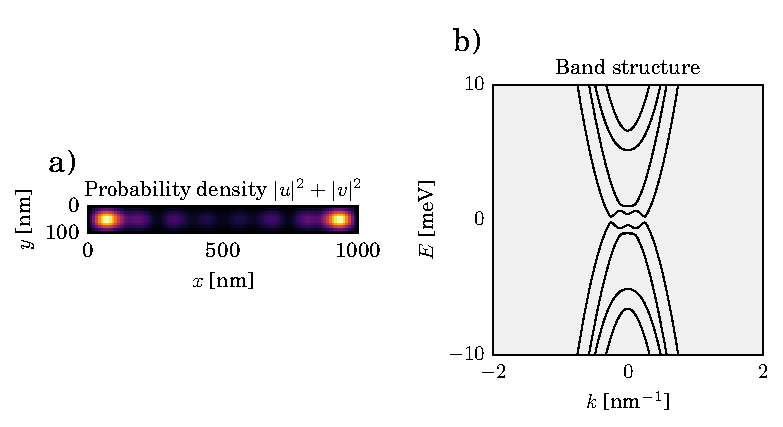
\includegraphics[width=0.95\textwidth]{chapter_introduction/figures/wavefunction_2d.pdf}
\caption{Similar to Fig~\ref{fig:wavefunction_1d}, but for a 2D system.
\label{fig:wavefunction_2d}}
\end{center}
\end{figure}




%%%%%%%%%%%%%%%%%%%%%%%%%%%%%%%%%%%%%%%%%%%%%%%%%%%%%%%%%%%%%%%%%%%%%%%%%%%%%%%%%%%%%%%
%%%%%%%%%%%%%%%%%%%%%%%%%%%%%%%%%% NUMERICAL METHODS %%%%%%%%%%%%%%%%%%%%%%%%%%%%%%%%%%
%%%%%%%%%%%%%%%%%%%%%%%%%%%%%%%%%%%%%%%%%%%%%%%%%%%%%%%%%%%%%%%%%%%%%%%%%%%%%%%%%%%%%%%


\section{Numerical methods}\label{sec:numerical_methods}

\subsection{Discretization of a Hamiltonian}

\subsection{Band structures}

\subsection{Smallest gap finding}

\subsection{Finding phase boundaries for systems where $\mu=\textrm{const.}$}



%%%%%%%%%%%%%%%%%%%%%%%%%%%%%%%%%%%%%%%%%%%%%%%%%%%%%%%%%%%%%%%%%%%%%%%%%%%%%%%%%%%%%%%
%%%%%%%%%%%%%%%%%%%%%%%%%%%%%% STRUCTURE OF THIS THESIS %%%%%%%%%%%%%%%%%%%%%%%%%%%%%%%
%%%%%%%%%%%%%%%%%%%%%%%%%%%%%%%%%%%%%%%%%%%%%%%%%%%%%%%%%%%%%%%%%%%%%%%%%%%%%%%%%%%%%%%


\section{Structure of this thesis}

Here, we give a brief overview of the topics explored in the following chapters.
\vspace{1mm}

\subsection{Chapter~\ref{ch:introduction}: Introduction}
Abstract here for introduction
\vspace{1mm}

\subsection{Chapter~\ref{ch:adaptive}: Title here for adaptive}
Abstract here for adaptive
\vspace{1mm}

\subsection{Chapter~\ref{ch:orbitalfield}: Orbital effect of magnetic field on the Majorana phase diagram}
Studies of Majorana bound states in semiconducting nanowires frequently neglect the orbital effect of a magnetic field.
Systematically studying its role leads us to several conclusions for designing Majoranas in this system.
Specifically, we show that for experimentally relevant parameter values the orbital effect of a magnetic field has a stronger impact on the dispersion relation than the Zeeman effect.
While Majoranas do not require the presence of only one dispersion subband, we observe that the size of the Majoranas becomes unpractically large, and the band gap unpractically small when more than one subband is filled.
Since the orbital effect of a magnetic field breaks several symmetries of the Hamiltonian, it leads to the appearance of large regions in parameter space with no band gap whenever the magnetic field is not aligned with the wire axis.
The reflection symmetry of the Hamiltonian with respect to the plane perpendicular to the wire axis guarantees that the wire stays gapped in the topologically nontrivial region as long as the field is aligned with the wire.
\vspace{1mm}

\subsection{Chapter~\ref{ch:supercurrent}: Supercurrent Interference in Few-Mode Nanowire Josephson Junctions}
Junctions created by coupling two superconductors via a semiconductor nanowire in the presence of high magnetic fields are the basis for the potential detection, fusion and braiding of Majorana bound states.
We study NbTiN/InSb nanowire/NbTiN Josephson junctions and find that the dependence of the critical current on the magnetic field exhibits gate-tunable nodes.
This is in contrast with a well-known Fraunhofer effect, under which critical current nodes form a regular pattern with a period fixed by the junction area.
Based on a realistic numerical model we conclude that the Zeeman effect induced by the magnetic field and the spin-orbit interaction in the nanowire are insufficient to explain the observed evolution of the Josephson effect.
We find the interference between the few occupied one-dimensional modes in the nanowire to be the dominant mechanism responsible for the critical current behavior.
We also report a strong suppression of critical currents at finite magnetic fields that should be taken into account when designing circuits based on Majorana bound states.
\vspace{1mm}

\subsection{Chapter~\ref{ch:spinorbit}: Spin-Orbit Protection of Induced Superconductivity in Majorana Nanowires}
Spin-orbit interaction (SOI) plays a key role in creating Majorana zero modes in semiconductor nanowires proximity coupled to a superconductor.
We track the evolution of the induced superconducting gap in InSb nanowires coupled to a NbTiN superconductor in a large range of magnetic field strengths and orientations.
Based on realistic simulations of our devices, we reveal SOI with a strength of 0.15--0.35 eV\AA.
Our approach identifies the direction of the spin-orbit field, which is strongly affected by the superconductor geometry and electrostatic gates.
\vspace{1mm}

\subsection{Chapter~\ref{ch:zigzag}: Title here for zigzag}
Abstract here for zigzag
\vspace{1mm}

\subsection{Chapter~\ref{ch:shortjunction}: Robustness of Majorana bound states in the short-junction limit}
We study the effects of strong coupling between a superconductor and a semiconductor nanowire on the creation of the Majorana bound states, when the quasiparticle dwell time in the normal part of the nanowire is much shorter than the inverse superconducting gap.
This ``short-junction'' limit is relevant for the recent experiments using the epitaxially grown aluminum characterized by a transparent interface with the semiconductor and a small superconducting gap.
We find that the small superconducting gap does not have a strong detrimental effect on the Majorana properties.
Specifically, both the critical magnetic field required for creating a topological phase and the size of the Majorana bound states are independent of the superconducting gap.
The critical magnetic field scales with the wire cross-section, while the relative importance of the orbital and Zeeman effects of the magnetic field is controlled by the material parameters only: $g$ factor, effective electron mass, and the semiconductor-superconductor interface transparency.



\references{dissertation}

\chapter{Adaptive, tools for adaptive parallel sampling of mathematical functions}
\label{ch:adaptive}

%% Start the actual chapter on a new page.
\newpage
\noindent
\hypertarget{introduction}{%
\section{Introduction}\label{introduction}}

\hypertarget{simulations-are-costly-and-often-require-sampling-a-region-in-parameter-space.}{%
\paragraph{Simulations are costly and often require sampling a region in parameter space.}\label{simulations-are-costly-and-often-require-sampling-a-region-in-parameter-space.}}

In the computational sciences, one often does costly simulations---represented by a function $f$---where a certain region in parameter space $X$ is sampled, mapping to a codomain $Y$: $f \colon X \to Y$.
Frequently, the different points in $X$ can be independently calculated.
Even though it is suboptimal, one usually resorts to sampling $X$ on a homogeneous grid because of its simple implementation.

\hypertarget{choosing-new-points-based-on-existing-data-improves-the-simulation-efficiency.}{%
\paragraph{Choosing new points based on existing data improves the simulation efficiency.}\label{choosing-new-points-based-on-existing-data-improves-the-simulation-efficiency.}}

An alternative, which improves the simulation efficiency, is to choose new potentially interesting points in $X$, based on existing data \cite{Gramacy2004, Figueiredo1995, Castro2008, Chen2017}.
Bayesian optimization works well for high-cost simulations where one needs to find a minimum (or maximum) \cite{Takhtaganov2018}.
However, if the goal of the simulation is to approximate a continuous function using the fewest points, the continuity of the approximation is achieved by a greedy algorithm that samples mid-points of intervals with the largest distance or curvature \cite{Wolfram2011}.
Such a sampling strategy (i.e., in Fig.~\ref{fig:algo}) would trivially speedup many simulations.
Here, the complexity arises when parallelizing this algorithm because this requires a lot of bookkeeping and planning.

\begin{figure}
\hypertarget{fig:algo}{%
\centering
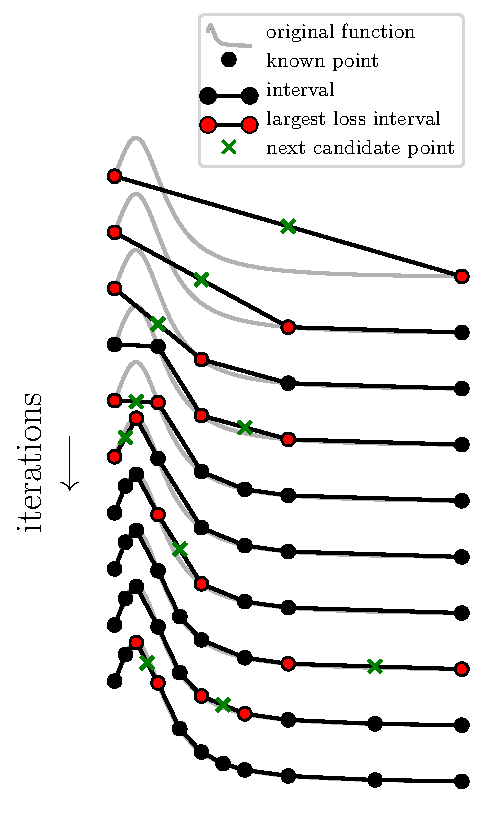
\includegraphics{chapter_adaptive/figures/algo.pdf}
\caption{Visualization of a 1-D point choosing algorithm for a black-box function (grey).
We start by calculating the two boundary points.
Two consecutive existing data points (black) $\{x_i, y_i\}$ define an interval.
Each interval has a loss $L_{i,i+1}$ associated with it that can be calculated from the points inside the interval $L_{i,i+1}(x_i, x_{i+1}, y_i, y_{i+1})$ and optionally of $N$ next nearest neighbouring intervals.
At each iteration the interval with the largest loss is indicated (red), with its corresponding candidate point (green) picked in the middle of the interval.
The loss function in this example is the curvature loss.}\label{fig:algo}
}
\end{figure}

\hypertarget{we-describe-a-class-of-algorithms-relying-on-local-criteria-for-sampling-which-allow-for-easy-parallelization-and-have-a-low-overhead.}{%
\paragraph{We describe a class of algorithms relying on local criteria for sampling, which allow for easy parallelization and have a low overhead.}\label{we-describe-a-class-of-algorithms-relying-on-local-criteria-for-sampling-which-allow-for-easy-parallelization-and-have-a-low-overhead.}}

To handle many parallel workers that calculate the function values and request new points, the algorithm needs to have a low computational overhead.
Requiring that, when a new point has been calculated, that the information updates are local (only in a region around the newly calculated point), will reduce the time complexity of the algorithm.
A simple example is greedily optimizing continuity of the sampling by selecting points according to the distance to the largest gaps in the function values, as in Fig.~\ref{fig:algo}.
For a one-dimensional function with three points known (its boundary points and a point in the center), such a simple algorithm consists of the following steps:
(1) keep all points $x$ sorted, where two consecutive points define an interval,
(2) calculate the distance for each interval $L_{i, i+1}=\sqrt{(x_{i+1}-x_{i})^{2}+(y_{i+1}-y_{i})^{2}}$,
(3) pick a new point $x_\textrm{new}$ in the middle of the interval with the largest $L$, creating two new intervals around that point,
(4) calculate $f(x_\textrm{new})$,
(5) repeat the previous steps, without redoing calculations for unchanged intervals.

In this paper, we present a class of algorithms that rely on local criteria for sampling, such as in the above example.
Here we associate a \emph{local loss} to each interval and pick a \emph{candidate point} inside the interval with the largest loss.
For example, in the case of the integration algorithm, the loss is the error estimate.
The advantage of these \emph{local} algorithms is that they allow for easy parallelization and have a low computational overhead.

\begin{figure}
\hypertarget{fig:Learner1D}{%
\centering
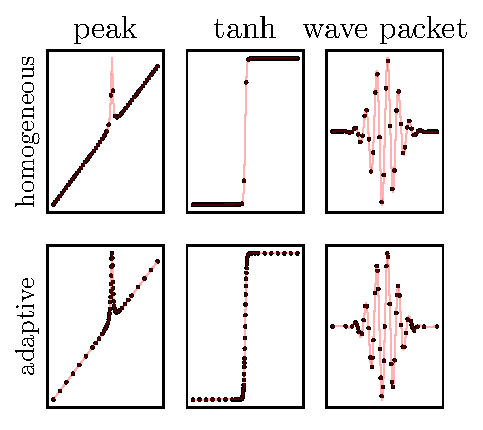
\includegraphics{chapter_adaptive/figures/Learner1D.pdf}
\caption{Comparison of homogeneous sampling (top) with adaptive sampling (bottom) for different one-dimensional functions (red) where the number of points in each column is identical.
We see that when the function has a distinct feature---such as with the peak and tanh---adaptive sampling performs much better.
When the features are homogeneously spaced, such as with the wave packet, adaptive sampling is not as effective as in the other cases.}\label{fig:Learner1D}
}
\end{figure}

\begin{figure}
\hypertarget{fig:Learner2D}{%
\centering
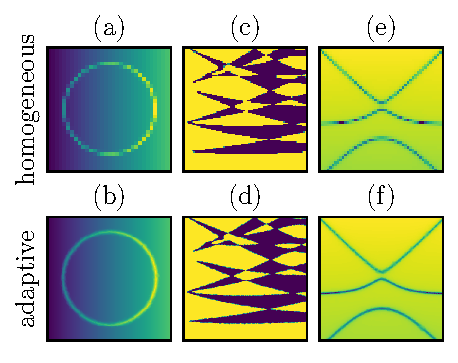
\includegraphics{chapter_adaptive/figures/Learner2D.pdf}
\caption{Comparison of homogeneous sampling (top) with adaptive sampling (bottom) for different two-dimensional functions where the number of points in each column is identical.
On the left is the function $f(x) = x + a ^ 2 / (a ^ 2 + (x - x_\textrm{offset}) ^ 2)$.
In the middle a topological phase diagram from \cite{Nijholt2016}, where the function can take the values -1 or 1.
On the right, we plot level crossings for a two-level quantum system.
In all cases using Adaptive results in a higher fidelity plot.}\label{fig:Learner2D}
}
\end{figure}

\hypertarget{we-provide-a-reference-implementation-the-adaptive-package-and-demonstrate-its-performance.}{%
\paragraph{We provide a reference implementation, the Adaptive package, and demonstrate its performance.}\label{we-provide-a-reference-implementation-the-adaptive-package-and-demonstrate-its-performance.}}

We provide a reference implementation, the open-source Python package called Adaptive \cite{Nijholt2019}, which has previously been used in several scientific publications \cite{Vuik2018, Laeven2019, Bommer2019, Melo2019}.
It has algorithms for $f \colon \mathbb{R}^N \to \mathbb{R}^M$, where $N, M \in \mathbb{Z}^+$ but which work best when $N$ is small; integration in $\mathbb{R}$; and the averaging of stochastic functions.
Most of our algorithms allow for a customizable loss function with which one can adapt the sampling algorithm to work optimally for different classes of functions.
It integrates with the Jupyter notebook environment as well as popular parallel computation frameworks such as \passthrough{\lstinline!ipyparallel!}, \passthrough{\lstinline!mpi4py!}, and \passthrough{\lstinline!dask.distributed!}.
It provides auxiliary functionality such as live-plotting, inspecting the data as the calculation is in progress, and automatically saving and loading of the data.

The raw data and source code that produces all plots in this paper is available at \cite{papercode}.

\hypertarget{sec:review}{%
\section{Review of adaptive sampling}\label{sec:review}}

Optimal sampling and planning based on data is a mature field with different communities providing their own context, restrictions, and algorithms to solve their problems.
To explain the relation of our approach with prior work, we discuss several existing contexts.
This is not a systematic review of all these fields, but rather, we aim to identify the important traits and design considerations.

\hypertarget{experiment-design-uses-bayesian-sampling-because-the-computational-costs-are-not-a-limitation.}{%
\paragraph{Experiment design uses Bayesian sampling because the computational costs are not a limitation.}\label{experiment-design-uses-bayesian-sampling-because-the-computational-costs-are-not-a-limitation.}}

Optimal experiment design (OED) is a field of statistics that minimizes the number of experimental runs needed to estimate specific parameters and, thereby, reduce the cost of experimentation \cite{Emery1998}.
It works with many degrees of freedom and can consider constraints, for example, when the sample space contains regions that are infeasible for practical reasons.
One form of OED is response-adaptive design \cite{Hu2006}, which concerns the adaptive sampling of designs for statistical experiments.
Here, the acquired data (i.e., the observations) are used to estimate the uncertainties of a certain desired parameter.
It then suggests further experiments that will optimally reduce these uncertainties.
In this step of the calculation Bayesian statistics is frequently used.
Bayesian statistics naturally provides tools for answering such questions; however, because it provides closed-form solutions, Markov chain Monte Carlo (MCMC) sampling is the standard tool for determining the most promising samples.
In a typical non-adaptive experiment, decisions on which experiments to perform are made in advance.

\hypertarget{plotting-and-low-dimensional-integration-uses-local-sampling.}{%
\paragraph{Plotting and low dimensional integration uses local sampling.}\label{plotting-and-low-dimensional-integration-uses-local-sampling.}}

Plotting a low dimensional function in between bounds requires one to evaluate the function on sufficiently many points such that when we interpolate values in between data points, we get an accurate description of the function values that were not explicitly calculated.
In order to minimize the number of function evaluations, one can use adaptive sampling routines.
For example, for one-dimensional functions, Mathematica \cite{WolframResearch} implements a \passthrough{\lstinline!FunctionInterpolation!} class that takes the function, $x_\textrm{min}$, and $x_\textrm{max}$, and returns an object that samples the function more densely in regions with high curvature; however, details on the algorithm are not published.
Subsequently, we can query this object for points in between $x_\textrm{min}$ and $x_\textrm{max}$, and get the interpolated value, or we can use it to plot the function without specifying a grid.
Another application for adaptive sampling is numerical integration.
It works by estimating the integration error of each interval and then minimizing the sum of these errors greedily.
For example, the \passthrough{\lstinline!CQUAD!} algorithm \cite{Gonnet2010} in the GNU Scientific Library \cite{Galassi1996} implements a more sophisticated strategy and is a doubly-adaptive general-purpose integration routine which can handle most types of singularities.
In general, it requires more function evaluations than the integration routines in \passthrough{\lstinline!QUADPACK!} \cite{Galassi1996}; however, it works more often for difficult integrands.
It is doubly-adaptive because it can decide to either subdivide intervals into more intervals or refine an interval by adding more points---that do not lie on a regular grid---to each interval.

\hypertarget{pde-solvers-and-computer-graphics-use-adaptive-meshing.}{%
\paragraph{PDE solvers and computer graphics use adaptive meshing.}\label{pde-solvers-and-computer-graphics-use-adaptive-meshing.}}

Hydrodynamics \cite{Berger1989, Berger1984} and astrophysics \cite{Klein1999} use an adaptive refinement of the triangulation mesh on which a partial differential equation is discretized.
By providing smaller mesh elements in regions with a higher variation of the solution, they reduce the amount of data and calculation needed at each step of time propagation.
The remeshing at each time step happens globally, and this is an expensive operation.
Therefore, mesh optimization does not fit our workflow because expensive global updates should be avoided.
Computer graphics uses similar adaptive methods where a smooth surface can represent a surface via a coarser piecewise linear polygon mesh, called a subdivision surface \cite{DeRose1998}.
An example of such a polygonal remeshing method is one where the polygons align with the curvature of the space or field; this is called anisotropic meshing \cite{Alliez2003}.

\hypertarget{design-constraints-and-the-general-algorithm}{%
\section{Design constraints and the general algorithm}\label{design-constraints-and-the-general-algorithm}}

\hypertarget{we-aim-to-sample-low-to-intermediate-cost-functions-in-parallel.}{%
\paragraph{We aim to sample low to intermediate cost functions in parallel.}\label{we-aim-to-sample-low-to-intermediate-cost-functions-in-parallel.}}

The general algorithm that we describe in this paper works best for low to intermediate cost functions.
The point suggestion step happens in a single sequential process while the function executions can be in parallel.
This means that to benefit from an adaptive sampling algorithm, that the time it takes to suggest a new point $t_\textrm{suggest}$ must be much smaller than the average function execution time $t_f$ over the number of parallel workers $N$: $t_f / N \gg t_\textrm{suggest}$.
Extremely fast functions can be calculated on a dense grid, and extremely slow functions might benefit from full-scale Bayesian optimization where $t_\textrm{suggest}$ is large.
We are interested in an intermediate case, when one may not fully run a fitting of all available data at each step; still, a large class of functions is inside the right regime for adaptive sampling to be beneficial.

\hypertarget{we-propose-to-use-a-local-loss-function-as-a-criterion-for-choosing-the-next-point.}{%
\paragraph{We propose to use a local loss function as a criterion for choosing the next point.}\label{we-propose-to-use-a-local-loss-function-as-a-criterion-for-choosing-the-next-point.}}

Because we aim to keep the suggestion time $t_\textrm{suggest}$ small, we propose to use a priority queue where we are keeping track of the subdomains containing candidate points (intervals in 1D.)
As we may not recompute this priority queue each time a new point is evaluated, only a fraction of the points can be updated.
That means that whatever priority we set to the points, it needs to be local.
We call this priority of each subdomain the loss, and it is determined only by the function values of the points inside that subdomain and optionally of its neighboring subdomains.
The loss then serves as a criterion for choosing the next point by virtue of choosing a new candidate point inside the subdomain with the maximum loss.
This means that upon adding new data points, only the intervals near the new point needs to have their loss value updated.
Due to the local nature of this algorithm and the sparsity of space in higher dimensions, we will suffer from the curse of dimensionality.
The algorithm, therefore, works best in low dimensional space; typically calculations that can reasonably be plotted, so with 1, 2, or 3 degrees of freedom.

The algorithm can be summarized as follows, where \passthrough{\lstinline!f!} is the function to evaluate, \passthrough{\lstinline!loss!} is the loss function, and \passthrough{\lstinline!heap\_push!}, \passthrough{\lstinline!head\_pop!} and \passthrough{\lstinline!heap\_max!} are functions for manipulating a max-heap.

\begin{lstlisting}
data $\gets$ empty_hashmap()
intervals $\gets$ empty_max_heap()
data[a] $\gets$ f(a)  # left bound
data[b] $\gets$ f(b)  # right bound
l $\gets$ loss(a, b, data[a], data[b])
heap_push(intervals, (l, a, b))

while heap_max(intervals)[0] > $\epsilon$:
  _, a, b $\gets$ heap_pop(intervals)
  m $\gets$ (a + b) / 2
  data[m] $\gets$ f(m)
  l_left $\gets$ loss(a, m, data[a], data[m])
  l_right $\gets$ loss(m, b, data[m], data[b])
  heap_push(intervals, (l_left, a, m))
  heap_push(intervals, (l_right, m, b))
\end{lstlisting}

In the above, \passthrough{\lstinline!loss!} only gets the data associated with a single interval;
in order to support loss functions that rely on data from neighboring intervals, we would need to maintain a separate data structure that encodes the neighborhood information.
For example, if \passthrough{\lstinline!data!} were a binary tree storing \passthrough{\lstinline!(x, f(x))!} then we could query neighboring points in $\mathcal{O}(\log n)$ time, where $n$ is the number of subdomains.

\hypertarget{as-an-example-the-interpoint-distance-is-a-good-loss-function-in-one-dimension.}{%
\paragraph{As an example, the interpoint distance is a good loss function in one dimension.}\label{as-an-example-the-interpoint-distance-is-a-good-loss-function-in-one-dimension.}}

An example of such a loss function for a one-dimensional function is the interpoint distance.
This loss will suggest to sample a point in the middle of an interval (subdomain) with the largest distance and thereby ensure the continuity of the function.
A more complex loss function that also takes the first neighboring intervals into account is one that adds more points where the second derivative (or curvature) is the highest.
Figure \ref{fig:Learner1D} shows a comparison between a result using this loss and a function that is sampled on a grid.

\hypertarget{with-many-points-due-to-the-loss-being-local-parallel-sampling-incurs-no-additional-cost.}{%
\paragraph{With many points, due to the loss being local, parallel sampling incurs no additional cost.}\label{with-many-points-due-to-the-loss-being-local-parallel-sampling-incurs-no-additional-cost.}}

So far, the description of the general algorithm did not include parallelism.
The parallel version of this algorithm proposes candidate points based on the existing data and the pending points.
To accommodate that, we replace the loss of subdomains that include pending points with an estimate based only on the evaluated data.
Adding a pending point to the dataset splits the subdomain to which it belongs into several smaller subdomains and assigns a fraction of the original loss to these subdomains as an estimate.
Providing the function value of a pending point then updates the loss estimate using the new data.
Because the loss function is local, $\mathcal{O}(1)$ subdomains are involved in both operations, therefore resulting in a $\mathcal{O}(1)$ computational cost.

\hypertarget{we-summarize-the-algorithm-with-pseudocode}{%
\paragraph{We summarize the algorithm with pseudocode}\label{we-summarize-the-algorithm-with-pseudocode}}

This is illustrated in the following algorithm, where \passthrough{\lstinline!parallel\_map!} takes a function and array of inputs and evaluates the function on each input in parallel, and \passthrough{\lstinline!n\_per\_round!} is the number of parallel evaluations to do at a time.

\begin{lstlisting}
def get_next(data, intervals):
  l, a, b, need_update $\gets$ heap_pop(intervals)
  while need_update:
    f_a $\gets$ data[a]
    f_b $\gets$ data[b]
    if f_a is None or f_b is None:
      break
    l $\gets$ loss(a, b, f_a, f_b)
    heap_push(intervals, (l, a, b, False))
    l, a, b, need_update $\gets$ heap_pop(intervals)
  return (l, a, b)


data $\gets$ empty_hashmap()
intervals $\gets$ empty_max_heap()
data[a] $\gets$ f(a)
data[b] $\gets$ f(b)
l $\gets$ loss(a, b, data[a], data[b])
heap_push(intervals, (l, a, b))

while heap_max(intervals)[0] > $\epsilon$:
  xs $\gets$ empty_array(n_per_round)
  for i in 0..n_per_round-1:
    l, a, b $\gets$ get_next(data, intervals)
    m $\gets$ (a + b) / 2
    xs[i] $\gets$ m
    heap_push(intervals, (l/2, a, m, True))
    heap_push(intervals, (l/2, m, b, True))

  fs $\gets$ parallel_map(f, xs)

  for i in 0..n_per_round:
    data[xs[i]] $\gets$ fs[i]
\end{lstlisting}

\hypertarget{the-parallel-algorithm-has-a-logarithmic-overhead-when-combined-with-an-appropriate-data-structure}{%
\paragraph{The parallel algorithm has a logarithmic overhead when combined with an appropriate data structure}\label{the-parallel-algorithm-has-a-logarithmic-overhead-when-combined-with-an-appropriate-data-structure}}

The key data structure in the parallel algorithm is the priority queue of subdomains.
It must support efficient removal and insertion, as well as finding the subdomain with the maximal loss.
An example of such a datastructure is a red--black tree or a skip list .
Both of these have an average complexity of $\mathcal{O}(\log{n})$ for all three operations.
In the reference implementation, we use the SortedContainers Python package that provides an efficient implementation of such a data structure optimized for realistic sizes, rather than asymptotic complexity.

\hypertarget{loss-function-design}{%
\section{Loss function design}\label{loss-function-design}}

\hypertarget{sampling-in-different-problems-pursues-different-goals}{%
\paragraph{Sampling in different problems pursues different goals}\label{sampling-in-different-problems-pursues-different-goals}}

\hypertarget{different-loss-functions-tailor-sampling-performance-to-different-goals}{%
\paragraph{Different loss functions tailor sampling performance to different goals}\label{different-loss-functions-tailor-sampling-performance-to-different-goals}}

The interpoint distance minimizing loss function we mentioned previously works on many functions; however, it is easy to write down a function where it will fail.
For example, $1/x^2$ has a singularity at $x=0$ and will be sampled too densely around that singularity using this loss.
We can avoid this by defining additional logic inside the loss function.

\hypertarget{adding-loss-functions-allows-for-balancing-between-multiple-priorities.}{%
\paragraph{Adding loss functions allows for balancing between multiple priorities.}\label{adding-loss-functions-allows-for-balancing-between-multiple-priorities.}}

Different loss functions prioritize sampling different features.
Adding loss functions allows for balancing between the multiple desired priorities.
For example, combining a loss function that calculates the curvature with a distance loss function, will sample regions with high curvature more densely, while ensuring continuity.

\hypertarget{loss-function-regularization-avoids-singularities}{%
\paragraph{Loss function regularization avoids singularities}\label{loss-function-regularization-avoids-singularities}}

To avoid indefinitely sampling the function based on a distance loss alone, we can regularize the loss.
A simple (but not optimal) strategy is to limit the size of each interval in the $x$ direction using,

\begin{equation*}
L_{i, i+1}^\textrm{dist}=\sqrt{(x_{i+1}-x_{i})^{2}+(y_{i+1}-y_{i})^{2}},
\end{equation*}

\begin{equation*}
L_{i,i+1}^\textrm{reg}=\begin{cases}
\begin{array}{c}
0\\
L_{i, i+1}^\textrm{dist}(x_i, x_{i+1}, y_i, y_{i+1})
\end{array} & \begin{array}{c}
\textrm{if} \; x_{i+1}-x_{i}<\epsilon,\\
\textrm{else,}
\end{array}\end{cases}
\end{equation*}

where $\epsilon$ is the smallest resolution we want to sample.

\hypertarget{asymptotically-dense-sampling-is-achieved-by-adding-subdomain-volume-to-the-loss}{%
\paragraph{Asymptotically dense sampling is achieved by adding subdomain volume to the loss}\label{asymptotically-dense-sampling-is-achieved-by-adding-subdomain-volume-to-the-loss}}

In two-dimensions (2D), subdomains are defined by triangles, where its vertices are known data points.
Losses are therefore calculated for each triangle but, unlike the 1D case, candidate points can be chosen at the center of one of the edges, instead of the center of the triangle, if the triangulation becomes better as a result.
A distance loss equivalent in 2D is the area spanned by the three-dimensional (3D) vectors of the vertices of the triangle.
Using this loss function, some narrow features in otherwise flat regions might not be discovered initially.
It is therefore beneficial if a loss function has a property that eventually, all points should be sampled.
A loss functions that ensure this is a homogeneous loss function that returns the 2D area span by the $x, y$ coordinates.
However, this loss function does not use the function-values and is, therefore, by itself is not an efficient solution.
Ideally, interesting regions are sampled more densely, while simultaneously new potentially interesting regions are also discovered.
By adding the two loss functions, we can combine the 3D area loss to exploit interesting regions, while the 2D area loss explores less densely sampled regions that might contain interesting features.

\hypertarget{examples}{%
\section{Examples}\label{examples}}

\hypertarget{line-simplification-loss}{%
\subsection{Line simplification loss}\label{line-simplification-loss}}

\hypertarget{the-line-simplification-loss-is-based-on-an-inverse-visvalingams-algorithm.}{%
\paragraph{The line simplification loss is based on an inverse Visvalingam's algorithm.}\label{the-line-simplification-loss-is-based-on-an-inverse-visvalingams-algorithm.}}

Inspired by a method commonly employed in digital cartography for coastline simplification, Visvalingam's algorithm, we construct a loss function that does its reverse \cite{Visvalingam1990}.
Here, at each point (ignoring the boundary points), we compute the effective area associated with its triangle, see Fig.~\ref{fig:line_loss}(b).
The loss then becomes the average area of two adjacent triangles.
By Taylor expanding $f$ around $x$ it can be shown that the area of the triangles relates to the contributions of the second derivative.
We can generalize this loss to $N$ dimensions, where the triangle is replaced by a $(N+1)$ dimensional simplex.

\begin{figure}
\hypertarget{fig:line_loss}{%
\centering
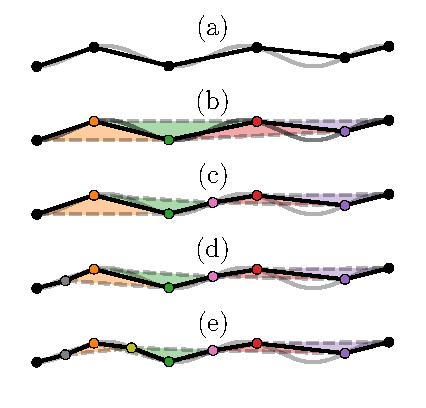
\includegraphics{chapter_adaptive/figures/line_loss.pdf}
\caption{Line loss visualization.
In this example, we start with 6 points (a) on the function (grey).
Ignoring the endpoints, the effective area of each point is determined by its associated triangle (b).
The loss of each interval can be computed by taking the average area of the adjacent triangles.
Subplots (c), (d), and (e) show the subsequent interations following (b).}\label{fig:line_loss}
}
\end{figure}

In order to compare sampling strategies, we need to define some error.
We construct a linear interpolation function $\tilde{f}$, which is an approximation of $f$.
We calculate the error in the $L^{1}$-norm, defined as,
\[
\text{Err}_{1}(\tilde{f})=\left\Vert \tilde{f}-f\right\Vert _{L^{1}}=\int_{a}^{b}\left|\tilde{f}(x)-f(x)\right|\text{d}x.
\]
This error approaches zero as the approximation becomes better.

\begin{figure}
\hypertarget{fig:line_loss_error}{%
\centering
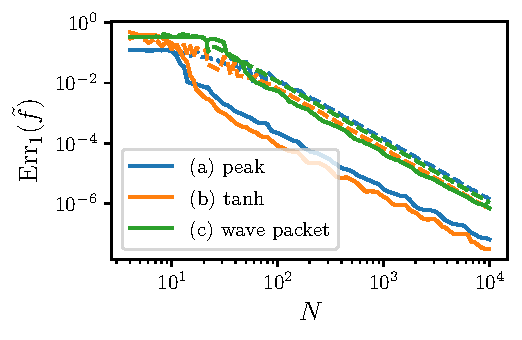
\includegraphics{chapter_adaptive/figures/line_loss_error.pdf}
\caption{The $L^{1}$-norm error as a function of number of points $N$ for the functions in Fig.~\ref{fig:Learner1D} (a,b,c).
The interrupted lines correspond to homogeneous sampling and the solid line to the sampling with the line loss.
In all cases adaptive sampling performs better, where the error is a factor 1.6-20 lower for $N=10000$.}\label{fig:line_loss_error}
}
\end{figure}

Figure \ref{fig:line_loss_error} shows this error as a function of the number of points $N$.
Here, we see that for homogeneous sampling to get the same error as sampling with a line loss, a factor $\approx 1.6-20$ times more points are needed, depending on the function.

\hypertarget{a-parallelizable-adaptive-integration-algorithm-based-on-cquad}{%
\subsection{A parallelizable adaptive integration algorithm based on cquad}\label{a-parallelizable-adaptive-integration-algorithm-based-on-cquad}}

\hypertarget{the-cquad-algorithm-belongs-to-a-class-that-is-parallelizable.}{%
\paragraph{\texorpdfstring{The \texttt{cquad} algorithm belongs to a class that is parallelizable.}{The cquad algorithm belongs to a class that is parallelizable.}}\label{the-cquad-algorithm-belongs-to-a-class-that-is-parallelizable.}}

In Sec.~\ref{sec:review} we mentioned the doubly-adaptive integration algorithm \passthrough{\lstinline!CQUAD!} \cite{Gonnet2010}.
This algorithm uses a Clenshaw-Curtis quadrature rules of increasing degree $d$ in each interval \cite{Clenshaw1960}.
The error estimate is $\sqrt{\int{\left(f_0(x) - f_1(x)\right)^2}}$, where $f_0$ and $f_1$ are two successive interpolations of the integrand.
To reach the desired total error, intervals with the maximum absolute error are improved.
Either (1) the degree of the rule is increased or (2) the interval is split if either the function does not appear to be smooth or a rule of maximum degree ($d=4$) has been reached.
All points inside the intervals can be trivially calculated in parallel; however, when there are more resources available than points, Adaptive needs to guess whether an (1) interval's should degree of the rule should be increased or (2) or the interval is split.
Here, we choose to always increase until $d=4$, after which the interval is split.

\hypertarget{isoline-and-isosurface-sampling}{%
\subsection{isoline and isosurface sampling}\label{isoline-and-isosurface-sampling}}

We can find isolines or isosurfaces using a loss function that prioritizes intervals that are closer to the function values that we are interested in.
See Fig.~\ref{fig:isoline}.

\begin{figure}
\hypertarget{fig:isoline}{%
\centering
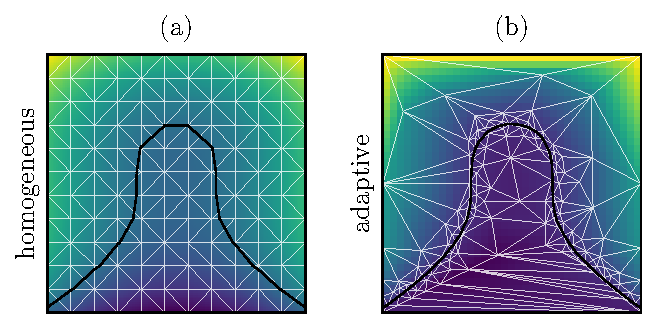
\includegraphics{chapter_adaptive/figures/isoline.pdf}
\caption{Comparison of isoline sampling of $f(x,y)=x^2 + y^3$ at $f(x,y)=0.1$ using homogeneous sampling (left) and adaptive sampling (right) with the same amount of points $n=17^2=289$.
We plot the function interpolated on a grid (color) with the triangulation on top (white) where the function is sampled on the vertices.
The solid line (black) indicates the isoline at $f(x,y)=0.1$.
The isoline in the homogeneous case consists of 62 line segments and the adaptive case consists of 147 line segments.}\label{fig:isoline}
}
\end{figure}

\hypertarget{implementation-and-benchmarks}{%
\section{Implementation and benchmarks}\label{implementation-and-benchmarks}}

\hypertarget{the-learner-abstracts-a-loss-based-priority-queue.}{%
\paragraph{The learner abstracts a loss based priority queue.}\label{the-learner-abstracts-a-loss-based-priority-queue.}}

We will now introduce Adaptive's API.
The object that can suggest points based on existing data is called a \emph{learner}.
The learner abstracts a loss based priority queue.
We can either \emph{ask} it for points or \emph{tell} the \emph{learner} new data points.
We can define a \emph{learner} as follows

\begin{lstlisting}[language=Python]
from adaptive import Learner1D

def peak(x): # pretend this is a slow function
    a = 0.01
    return x + a**2 / (a**2 + x**2)

learner = Learner1D(peak, bounds=(-1, 1))
\end{lstlisting}

\hypertarget{the-runner-orchestrates-the-function-evaluation.}{%
\paragraph{The runner orchestrates the function evaluation.}\label{the-runner-orchestrates-the-function-evaluation.}}

To drive the learner manually (not recommended) and sequentially, we can do

\begin{lstlisting}[language=Python]
def goal(learner):
    # learner.loss() = max(learner.losses)
    return learner.loss() < 0.01

while not goal(learner):
    points, loss_improvements = learner.ask(n=1)
    for x in points:  # len(points) == 1
        y = f(x)
        learner.tell(x, y)
\end{lstlisting}

To do this automatically (recommended) and in parallel (by default on all cores available) use

\begin{lstlisting}[language=Python]
from adaptive import Runner
runner = Runner(learner, goal)
\end{lstlisting}

This will return immediately because the calculation happens in the background.
That also means that as the calculation is in progress, \passthrough{\lstinline!learner.data!} is accessible and can be plotted with \passthrough{\lstinline!learner.plot()!}.
Additionally, in a Jupyter notebook environment, we can call \passthrough{\lstinline!runner.live\_info()!} to display useful information.
To change the loss function for the \passthrough{\lstinline!Learner1D!} we pass a loss function, like

\begin{lstlisting}[language=Python]
def distance_loss(xs, ys): # used by default
    dx = xs[1] - xs[0]
    dy = ys[1] - ys[0]
    return np.hypot(dx, dy)

learner = Learner1D(peak, bounds=(-1, 1), loss_per_interval=distance_loss)
\end{lstlisting}

Creating a homogeneous loss function is as simple as

\begin{lstlisting}[language=Python]
def uniform_loss(xs, ys):
    dx = xs[1] - xs[0]
    return dx

learner = Learner1D(peak, bounds=(-1, 1), loss_per_interval=uniform_loss)
\end{lstlisting}

We have also implemented a \passthrough{\lstinline!LearnerND!} with a similar API

\begin{lstlisting}[language=Python]
from adaptive import LearnerND

def ring(xy): # pretend this is a slow function
    x, y = xy
    a = 0.2
    return x + np.exp(-(x**2 + y**2 - 0.75**2)**2/a**4)

learner = adaptive.LearnerND(ring, bounds=[(-1, 1), (-1, 1)])
runner = Runner(learner, goal)
\end{lstlisting}

Again, it is possible to specify a custom loss function using the \passthrough{\lstinline!loss\_per\_simplex!} argument.

\hypertarget{the-balancinglearner-can-run-many-learners-simultaneously.}{%
\paragraph{The BalancingLearner can run many learners simultaneously.}\label{the-balancinglearner-can-run-many-learners-simultaneously.}}

Frequently, more than one function (learner) needs to run at once, to do this we have implemented the \passthrough{\lstinline!BalancingLearner!}, which does not take a function, but a list of learners.
This learner internally asks all child learners for points and will choose the point of the learner that maximizes the loss improvement; thereby, it balances the resources over the different learners.
We can use it like

\begin{lstlisting}[language=Python]
from functools import partial
from adaptive import BalancingLearner

def f(x, pow):
    return x**pow

learners = [Learner1D(partial(f, pow=i)), bounds=(-10, 10) for i in range(2, 10)]
bal_learner = BalancingLearner(learners)
runner = Runner(bal_learner, goal)
\end{lstlisting}

For more details on how to use Adaptive, we recommend reading the tutorial inside the documentation \cite{Nijholt2018}.

\hypertarget{possible-extensions}{%
\section{Possible extensions}\label{possible-extensions}}

\hypertarget{anisotropic-triangulation-would-improve-the-algorithm.}{%
\paragraph{Anisotropic triangulation would improve the algorithm.}\label{anisotropic-triangulation-would-improve-the-algorithm.}}

The current implementation of choosing the candidate point inside a simplex (triangle in 2D) with the highest loss, for the \passthrough{\lstinline!LearnerND!}, works by either picking a point (1) in the center of the simplex or (2) by picking a point on the longest edge of the simplex.
The choice depends on the shape of the simplex, where the algorithm tries to create regular simplices.
Alternatively, a good strategy is choosing points somewhere on the edge of a triangle such that the simplex aligns with the gradient of the function; creating an anisotropic triangulation \cite{Dyn1990}.
This is a similar approach to the anisotropic meshing techniques mentioned in the literature review.

\hypertarget{learning-stochastic-functions-is-a-promising-direction.}{%
\paragraph{Learning stochastic functions is a promising direction.}\label{learning-stochastic-functions-is-a-promising-direction.}}

Stochastic functions frequently appear in numerical sciences.
Currently, Adaptive has a \passthrough{\lstinline!AverageLearner!} that samples a stochastic function with no degrees of freedom until a certain standard error of the mean is reached.
This is advantageous because no predetermined number of samples has to be set before starting the simulation.
Extending this learner to be able to deal with more dimensions would be a useful addition.

\hypertarget{experimental-control-needs-to-deal-with-noise-hysteresis-and-the-cost-for-changing-parameters.}{%
\paragraph{Experimental control needs to deal with noise, hysteresis, and the cost for changing parameters.}\label{experimental-control-needs-to-deal-with-noise-hysteresis-and-the-cost-for-changing-parameters.}}

Finally, there is the potential to use Adaptive for experimental control.
Experiments often deal with noise, which could be solved by taking multiple measurements and averaging over the outcomes, such as the (not yet existing) \passthrough{\lstinline!AverageLearnerND!} will do.
Another challenge in experiments is that changing parameters can be slow.
Sweeping over one dimension might be faster than in others; for example, in condensed matter physics experiments, sweeping the magnetic field is much slower than sweeping frequencies.
Additionally, some experiments exhibit hysteresis, which means that the sampling direction has to be restricted to certain paths.
All these factors have to be taken into account to create a general-purpose sampler that can be used for experiments.
However, Adaptive can already be used in experiments that are not restricted by the former effects.

\references{dissertation}
\chapter{Orbital effect of magnetic field on the Majorana phase diagram}
\label{ch:orbitalfield}

%% Start the actual chapter on a new page.
\newpage
\noindent 
\section{Introduction}

\section{Introduction}
The search for Majorana bound states, the simplest non-Abelian particles, is fueled by their suitability for fault-tolerant quantum computation~\cite{Alicea2012,Beenakker2013}.
A large fraction of the experimental effort~\cite{Mourik2012,Das2012,Deng2012,Churchill2013,Deng2014} is focused on creating Majoranas in semiconducting nanowires with proximity superconductivity, spin-orbit coupling, and magnetic field.
The theoretical foundation for this platform was initially developed for a single one-dimensional spinful band with intrinsic superconducting pairing~\cite{Lutchyn2010,Oreg2010}.
Due to its compactness this model can be solved analytically, and it predicts that Majorana bound states appear when $E_\textrm{Z}^{2}>\mu^{2}+\Delta^{2}$, when the Zeeman energy becomes larger than the harmonic mean of the superconducting gap and the chemical potential.

% \comment{Model is too simple and generalizations have been made.}
The single-mode model is minimalistic and neglects many physical phenomena that are crucial for understanding the properties of the Majorana bound states.
The existing extensions of this model study multimode wires~\cite{Potter2010}, better modeling of the induced gap~\cite{Liu2012,Stanescu2014}, the role of electrostatics~\cite{Vuik2016}, disorder~\cite{Potter2012,Pientka2012,Adagideli2014}, and the $k \cdot p$-model~\cite{Stanescu2013}.
The orbital effect of a magnetic field was analyzed both in planar wires~\cite{Osca2015, Lim2012} and on the surface of a cylinder~\cite{Lim2013}.

% \comment{We include orbital effects.}
We systematically study the influence of the orbital effect of a magnetic field on the symmetries of the Hamiltonian and the topological phase diagram for a three-dimensional (3D) nanowire.
The orbital effect of a magnetic field perpendicular to the wire induces a skipping orbit motion of the electrons.
The cyclotron radius becomes comparable to the typical wire diameters $d \sim \SI{100}{\nano\metre}$ already at the field of $\SI{0.3}{\tesla}$, and at chemical potential corresponding to the optimal topological band gap.
In addition, a field parallel to the wire shifts the energies of each band due to the effect of magnetic flux.
We expect the shift of the energies to be comparable to the level spacing when the flux through the wire diameter is of the order of a flux quantum.
Our findings are very different from those of Refs.~\onlinecite{Osca2015, Lim2013, Lim2012} because we do not limit our analysis to a Hamiltonian with an artificially high spatial symmetry, or low dimensionality.


\section{Model}

% \comment{We consider a three-dimensional nanowire with a Rashba-BdG Hamiltonian.}

We consider a 3D semiconducting nanowire with Rashba spin-orbit coupling and proximity-induced s-wave superconductivity.
The nanowire cross section is a regular hexagon, and the nanowire is translationally invariant in the $x$-direction.
Its Bogoliubov-de Gennes Hamiltonian (BdG) is
\begin{eqnarray}
H_\textrm{BdG} & = & \left(\frac{\bm{p}^{2}}{2m^*}-\mu\right)\tau_z+\alpha\left(p_{y}\sigma_x -p_{x}\sigma_y \right)\tau_z\nonumber \\
 &  & +\frac{1}{2}g\mu_\textrm{B}\bm{B}\cdot\boldsymbol{\sigma}+\Delta\tau_x,\label{eq:H_BdG}
\end{eqnarray}
and it acts on the spinor wave function $\Psi={\left(\psi_{e\uparrow},\psi_{e\downarrow},\psi_{\textrm{h}\downarrow},-\psi_{\textrm{h}\uparrow}\right)}^{T}$, where $\psi_e$, $\psi_\textrm{h}$ are its electron and hole components, and $\psi_\uparrow$, $\psi_\downarrow$ are the spin-up and spin-down components.
We introduced the Pauli matrices $\sigma_{i}$ acting on the spin degree of freedom and $\tau_{i}$ acting on the electron-hole degree of freedom.
Further $\bm{p}=-i\hbar\nabla+e\bm{A}\tau_z$ is the canonical momentum, with $e$ the electron charge and the vector potential $\bm{A}={\left[ B_y (z - z_0) - B_z (y - y_0), 0, B_x (y - y_0)\right]}^{T}$ chosen such that it does not depend on $x$.
We set the offsets $y_0$ and $z_0$ to ensure that the average vector potential vanishes in the superconductor.
This choice corresponds to a limit when the superconductor is thinner than the screening length and its total supercurrent is zero, appropriate for existing devices.
Finally, $m^*$ is the effective electron mass, $E_\textrm{Z}=\mu_\textrm{B}g\bm{B}\cdot\boldsymbol{\sigma}/2$ the Zeeman energy,  $\Delta$ the superconducting pairing potential, $\alpha$ the Rashba spin-orbit coupling strength, and $\mu=\mu_0+\mathcal{E} z$ the chemical potential created by a constant electric field $\mathcal{E}$ in the sample parallel to the $z$\kern-.05ex-axis, such that the Rashba spin-orbit acts in the $xy$\kern-.05ex-plane.

% \comment{The pairing is either intrinsic or attached laterally.}

First we consider a model with a constant superconducting gap $\Delta$ inside the wire [see Fig.~\ref{fig:geometry}(a)] and then proceed to make a more realistic model of the superconductor.
To do that we set the superconducting order parameter $\Delta$ to zero in the wire and add a superconductor to the top which covers $3/8$ of the circumference of the wire [see Fig.~\ref{fig:geometry}(b)].
We choose the thickness of the superconductor to be $\SI{20}{\nano\metre}$ and set $\Delta$ in the superconductor such that the induced gap of the lowest band is $\Delta_\textrm{ind}=\SI{0.250}{\milli\electronvolt}$.
This is done by computing band energies at $k=0$ over a range of $\mu$ and matching the minimum to $\Delta_\textrm{ind}$.
We add a tunnel barrier between the two materials to change the transparency of the superconductor.
In the setup of Fig.~\ref{fig:geometry}(c), we break the reflection symmetry with respect to the $xz$-plane by moving the superconductor to the side similar to the experimental setup of Mourik \emph{et al}~\cite{Mourik2012}.

% \comment{We discretize the model and simulate it with Kwant.}

To perform the numerical simulations we discretize the Hamiltonian on a cubic lattice with lattice constant $a=\SI{10}{\nano\metre}$, much smaller than the minimal Fermi wavelength in the parameter range we consider.
The discretization does not break or introduce any additional symmetries.
The Hamiltonian at a lattice momentum $k$ equals $H\left(k\right)=h+t\exp(ik)+t^{\dagger}\exp(-ik)$ where $h$ is the Hamiltonian of the cross section of the tight-binding system and $t$ is the hopping matrix between the neighboring cross sections.
We introduce the vector potential by Peierls substitution $t_{nm}\rightarrow t_{nm}\exp(-ie\intop\bm{A}d\bm{l})$~\cite{Hofstadter1976}.
We perform the numerical simulations using the Kwant code~\cite{Groth2014}.
The source code and the specific parameter values are available in the Supplemental Material~\cite{supp}. 
The resulting raw data are available in Ref.~\onlinecite{data}.


\section{Symmetry analysis}

% \comment{The fundamental symmetry of the Majoranas is class D, but it does not allow reliable creation of topological gap because it allows for the tilting of the bands.}

The Majorana bound states are protected by the combination of the band gap and the particle-hole symmetry of the Hamiltonian $\mathcal{P}H\left(k\right)\mathcal{P}^{-1}=-H\left(-k\right)$.
In the basis of Eq.~\eqref{eq:H_BdG} this symmetry has the form $\mathcal{P}=\sigma_y \tau_y\mathcal{K}$, with $\mathcal{K}$ the complex conjugation.
In general there are no additional symmetries and the Hamiltonian belongs to symmetry class D~\cite{Altland1997}.
Particle-hole symmetry only requires that the energy $E_n(k)$ of $n$-th band at momentum $k$ is $E_n(k)=-E_m(-k)$ of some other $m$-th band; at the same time $\mathcal{P}$ puts no constraints on $E_n$ itself.
This means that whenever $E_{n}$ changes sign at a certain momentum, the band structure becomes gapless.
This tilting of the band structure~\cite{Rex2014} [shown in the middle panels in Fig.~\ref{fig:bandstructure}, where $E_n(k) \ne -E_m(k)$] is a strong effect that does not vanish with superconducting gap or spin-orbit, and can easily become larger than the induced gap, rendering the creation of Majoranas impossible.

% \comment{In the existing models have an extra chiral symmetry that prevents tilting, but it is broken by the orbital part of magnetic field.}

The tilting of the band structure is absent if the Hamiltonian has an extra chiral symmetry alongside $\mathcal{P}$.
It has been shown that the Hamiltonian has an approximate chiral symmetry $\mathcal{C}H\left(k\right)\mathcal{C}^{-1}=-H\left(k\right)$, $\mathcal{C}=\sigma_y \tau_y$, valid when the wire diameter $d$ is smaller than the spin-orbit length $l_{so}=\hbar^{2}/m^{*}\alpha$~\cite{Tewari2012,Diez2012}, and $B_y=0$.
Then the $p_{y}\sigma_x \tau_z$ term, associated with the transverse motion in Eq.~\eqref{eq:H_BdG}, is negligible.
Without the tilting, the system is gapped in every region of parameter space, except at the topological phase boundaries.
However, for relevant experimental parameters~\cite{Mourik2012}, the orbital terms break this symmetry more strongly than the spin-orbit term, bringing the system back to symmetry class D.

% \comment{We find that there is a reflection symmetry that guarantees the absence of tilting for field in $x$.}

We perform a systematic search of symmetries that the Hamiltonian~\eqref{eq:H_BdG} may have.~\cite{rosdahl}
We find the reflection symmetry with respect to the $yz$-plane $\mathcal{R}_x H\left(k\right)\mathcal{R}_x^{-1}=H\left(-k\right)$, $\mathcal{R}_x=\sigma_x\delta(x+x')$.
It is independent of the wire geometry and spin-orbit strength and guarantees the absence of tilting whenever the field is aligned with the $x$-axis.
The combined symmetry $\mathcal{P}' = \mathcal{R}_x \mathcal{P}$ is local in momentum space and ensures the absence of band structure tilting: $\mathcal{P}' H(k) \mathcal{P}'^{-1} = -H(k)$.

% \comment{Additionally, if the system has a reflection symmetry along the $y$-axis, there is an extra chiral symmetry that is valid for fields in the complete $xz$-plane.}

Additionally, we find a chiral symmetry $\mathcal{C}'=\tau_y\mathcal{R}_y$, $\mathcal{C}'H\left(k\right)\mathcal{C}'^{-1}=-H\left(k\right)$, with $\mathcal{R}_y = \sigma_y \delta(y + y')$ the reflection with respect to the $y$-axis.
This chiral symmetry holds when the magnetic field lies in the $xz$-plane and none of the potentials in Eq.~\eqref{eq:H_BdG} break $\mathcal{R}_y$, like in the setups of Figs.~\ref{fig:geometry}(a) and\ref{fig:geometry}(b).
When present, $\mathcal{C}'$ guarantees the absence of band structure tilting just like $\mathcal{C}$.
This symmetry is present in most theoretical models, and in particular it is obeyed by the Hamiltonians used in Refs.~\onlinecite{Osca2015, Lim2013, Lim2012}.
A finite $B_y$ breaks both $\mathcal{R}_x$ and $\mathcal{C}'$ therefore, the bands can tilt and close the topological gap.
The band structures in Fig.~\ref{fig:bandstructure} summarize the relation between the geometry of the setup of Figs~\ref{fig:geometry}(b) and Fig.~\ref{fig:geometry}(c), magnetic field orientation, and the symmetries of the Hamiltonian.

\begin{figure}
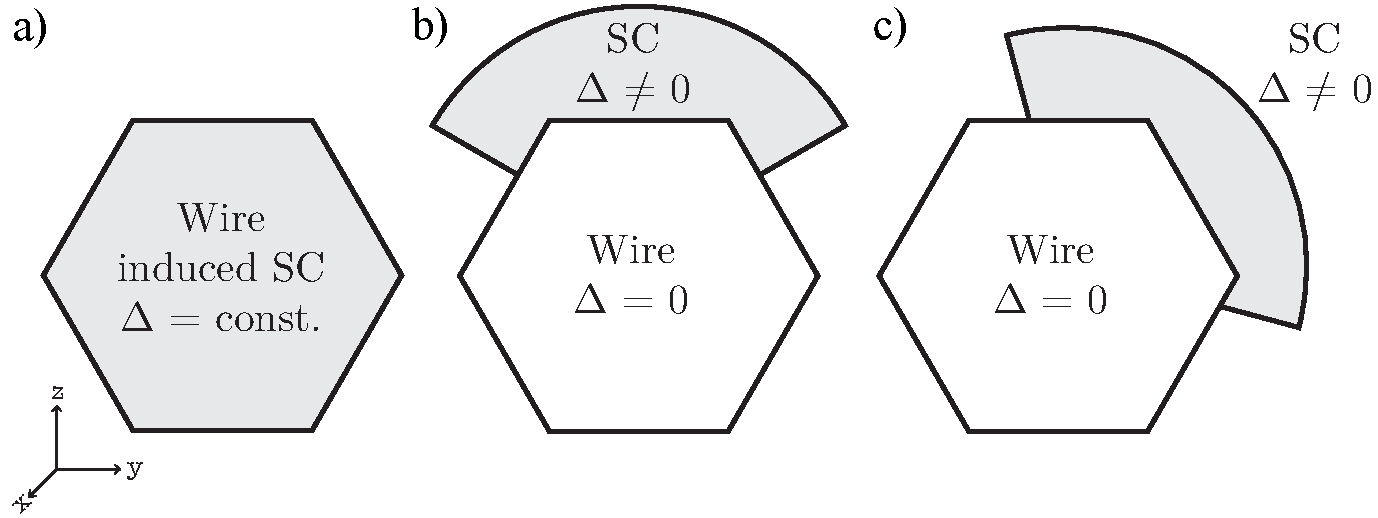
\includegraphics[width=0.95\columnwidth]{figures/geometry}
\caption{Three hexagonal nanowire devices we consider: (a) (a) with an intrinsic pairing term and with a proximity-coupled superconductor (b) on the top and (c) on the side.
The last two setups have tunnel barriers between the superconductor and the nanowire.
\label{fig:geometry}}
\end{figure}

\begin{figure}
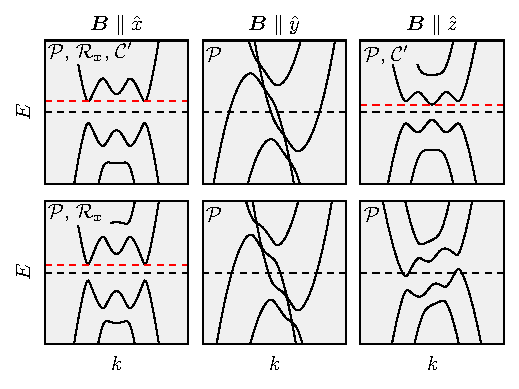
\includegraphics[width=0.95\columnwidth]{figures/bandstructure_annotated}
\caption{Band structures of the setup of Fig.~\ref{fig:geometry}(b) (top) and Fig.~\ref{fig:geometry}(c) (bottom).
Each panel is labeled with the symmetries respected by the corresponding Hamiltonian.
The dashed black line indicates the Fermi energy $(E=0)$.
The red dashed lines show the size of the band gap if it is present.
In the top row, the reflection symmetry of the wire along the $y$-axis $\mathcal{R}_y$ makes the Hamiltonian have a chiral symmetry $\mathcal{C}'$ when the magnetic field lies in the $xz$-plane.
The wire used for the calculation of the bottom row dispersions lacks $\mathcal{R}_y$ and therefore has no $\mathcal{C}'$.
Without $\mathcal{C}'$ the bands are allowed to tilt and the gap may close whenever $B_y \neq 0$ or $B_z \neq 0$.
A magnetic field parallel to the $x$-axis preserves $\mathcal{R}_x$, which protects the band gap from closing.\label{fig:bandstructure}}
\end{figure}

\section{Calculating the topological phase diagram}

% \comment{We use a generalized eigenvalue problem to find all phase boundaries at once.}

We use an optimized algorithm to quickly find all the $\mu$ values corresponding to the topological phase transitions at once.
The topological transitions in symmetry class D occur when $\Pf H_\textrm{BdG}(k=0)$ changes sign.
\footnote{The band gap closings at $k=\pi$ can be treated identically, but they never appear in our model Hamiltonian.}
Since the sign change of $\Pf H_\textrm{BdG}$ is accompanied by the appearance of zero energy states, we need to find $\mu$ and $\psi$ such that $H(\mu, k=0)\psi = 0$.
Using that $\mu$ enters the Hamiltonian as a prefactor of a linear operator, we rewrite this equation as a generalized eigenproblem:
\begin{eqnarray}
H_\textrm{BdG}\left(\mu=0,k=0\right)\psi=\mu\tau_z\psi.\label{eq:eigenproblem}
\end{eqnarray}
The real eigenvalues of this eigenproblem are the values of $\mu$ where the gap closes at $k=0$ [see Fig.~\ref{fig:ev_problem}(a)], and they can be found using standard generalized eigensolvers.
If the dispersion relation is gapped also at any finite $k$, these gap closings are the boundaries of the topological phase.

\begin{figure}
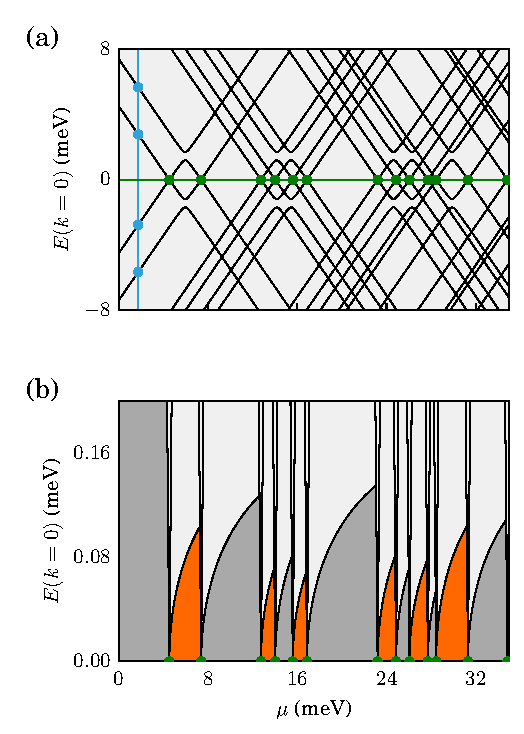
\includegraphics[width=0.95\columnwidth]{figures/ev_problem}
\caption{(a) Energy spectrum at $k=0$ of the setup of Fig.\ref{fig:geometry}(a) as a function of chemical potential $\mu$.
The blue points are the solutions of $H_\textrm{BdG} \psi = E \psi$ at fixed $\mu$ marked by the blue line.
The green points are the real eigenvalues of Eq.~\eqref{eq:eigenproblem} lying at $E=0$ (the green line).
(b) The gap size for the same setup and parameters, with dark gray regions trivial and the orange regions topological.\label{fig:ev_problem}}
\end{figure}

Since the eigenvalues of $H_\textrm{BdG}$ come in opposite sign pairs, the real eigenvalues of Eq.~\eqref{eq:eigenproblem} always come in degenerate pairs, and each pair lies at a transition between a trivial and a nontrivial phase.
We complete the calculation of the topological phase diagram by using as a reference point that $H_\textrm{BdG}(\mu = -\infty)$ is topologically trivial.

\begin{figure}
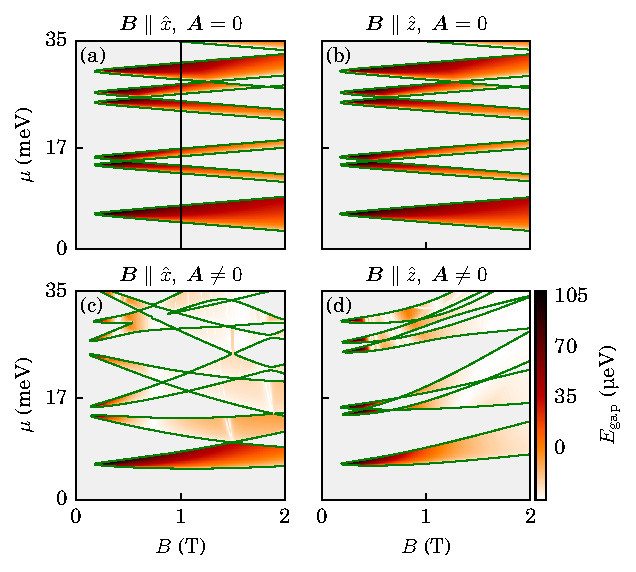
\includegraphics[width=0.95\columnwidth]{figures/comparing_phase_diagrams}
\caption{Phase diagrams of the setup of Fig.~\ref{fig:geometry}(a) (a), (b) without
the orbital effect of a magnetic field and (c), (d) with it.
The green lines depict the topological phase transitions.
The colored regions are topologically nontrivial, with the color representing the size of the topological band gap $E_\textrm{gap}$.
At $B \gtrsim \SI{1}{\tesla}$ the orbital effect of the magnetic field becomes stronger than the Zeeman effect and changes the sign of the slope of half of the phase boundaries.
Furthermore, the orbital effect leads to a faster suppression of the band gaps with magnetic field.\label{fig:phase-diagrams}
The narrow regions with suppressed $E_\textrm{gap}$ originating from the crossings of the phase boundaries in (c) are due to Dirac cones appearing in $(k_x, B)$\!-space and are protected by $C'$.
The vertical black line in (a) indicates the value of the magnetic field used in Fig.~\ref{fig:ev_problem}.}
\end{figure}

% \comment{We calculate the gap by performing a binary search for the energy at which propagating modes appear.}

The generalized eigenvalue algorithm for finding phase boundaries does not guarantee that $H(k)$ is gapped for $k \neq 0$, and therefore we calculate the magnitude of the gap $E_\textrm{gap}$ in the topologically nontrivial regime separately for each set of parameter values.
We form a translation eigenvalue problem to calculate all the modes of $H_\textrm{BdG}$ at a given energy $E$ and check whether there are any propagating modes~\cite{Groth2014}.
By using a binary search in $E$ for the energy at which the propagating modes start to appear, we find $E_\textrm{gap}$ [see Fig.~\ref{fig:ev_problem}(b)].

% \comment{We find the Majorana lengths by calculating the slowest decaying mode.}

The real space size of the Majoranas $\xi$ imposes a lower bound on the nanowire length required to create them.
To calculate $\xi$ we find the eigenvalue decomposition of the translation operator at zero energy.
The eigenvalue $\lambda_{\min}$ closest to the unit circle corresponds to the slowest decaying part of the Majorana wave function.
We calculate $\xi$ using
\begin{equation}
\xi=\abs{\log^{-1}\abs{\lambda_{\min}}}.
\end{equation}

\begin{figure}
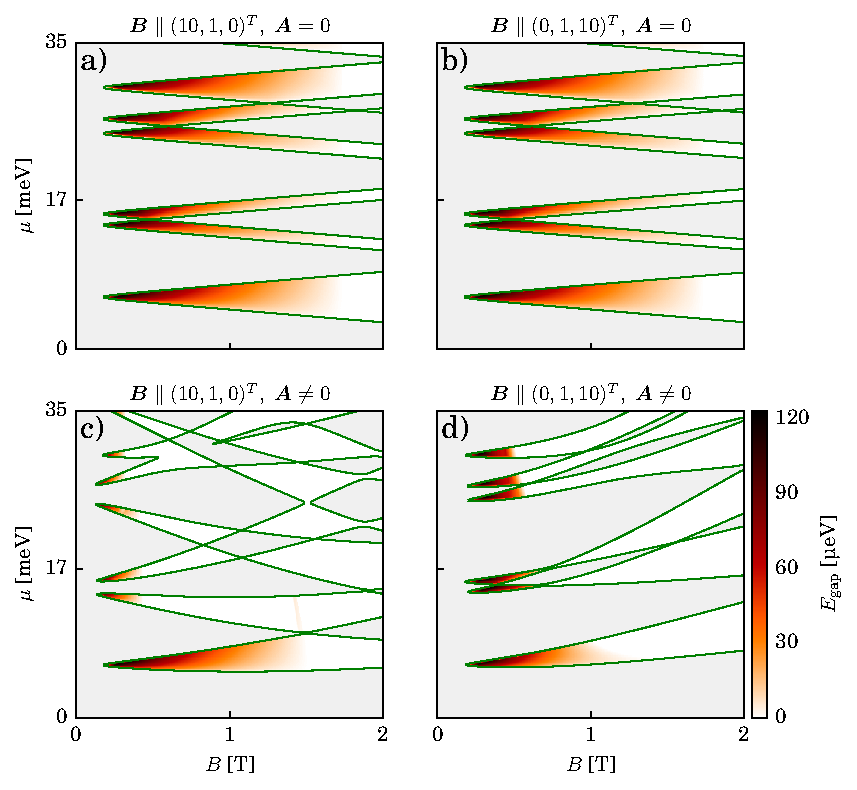
\includegraphics[width=0.95\columnwidth]{figures/misaligned}
\caption{Same as Fig.~\ref{fig:phase-diagrams}, but with the magnetic field slightly misaligned.
We observe that the band gaps close quickly upon changing the direction of the magnetic field towards the spin-orbit direction in $y$.
\label{fig:misaligned}}
\end{figure}

\begin{figure}
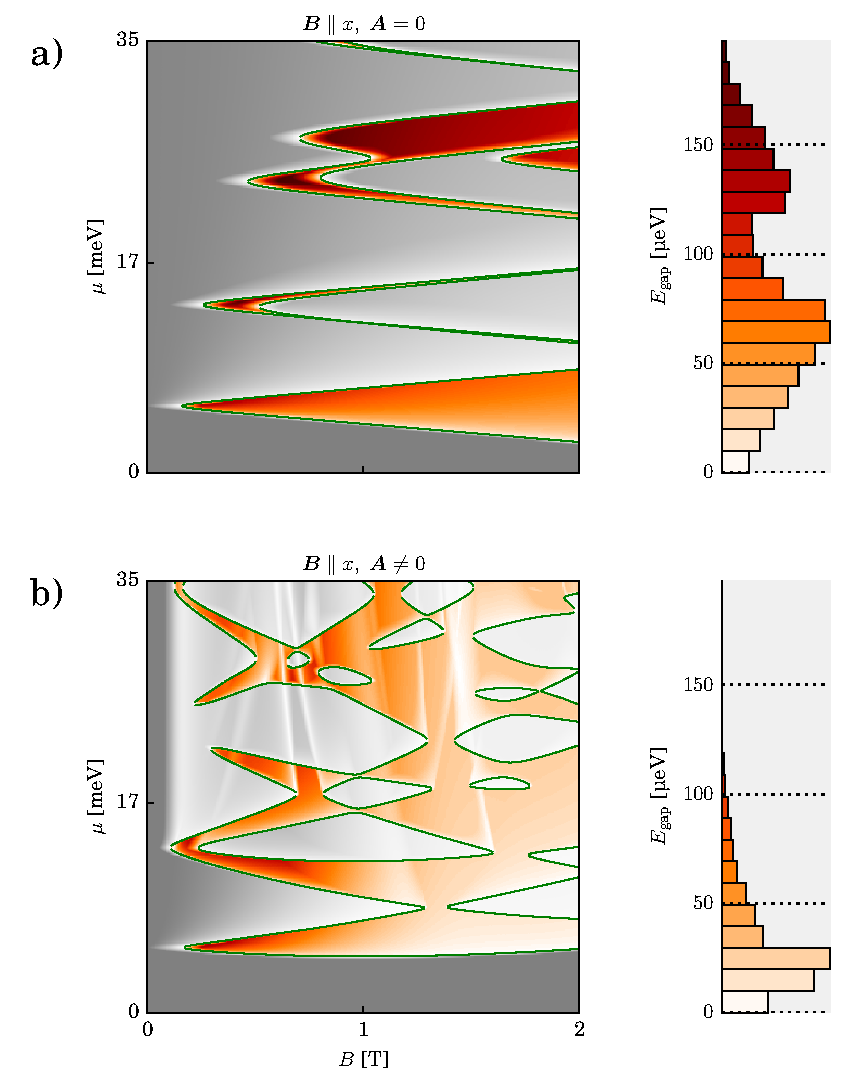
\includegraphics[width=0.95\columnwidth]{figures/sc_on_side_hist}
\caption{Phase diagrams of the setup of Fig.~\ref{fig:geometry}(c) (a) without the orbital effect of a magnetic field and (b) with it. Color scale corresponds to $E_\textrm{gap}$, with the topological regions colored and trivial regions in grayscale.
The histograms in the right-hand panels show the distribution of the gap values sampled in the topological regime within the selected parameter range. 
Neglecting the orbital effect of the magnetic field incorrectly leads to a strong dependence of the critical field on $\mu$.
With the orbital effect of magnetic field flux penetration through the quasiparticle trajectory changes the interference phases and can suppress the topological gap $E_\textrm{gap}$.
\label{fig:phase-diagram-sc_on_side}}
\end{figure}

\begin{figure}
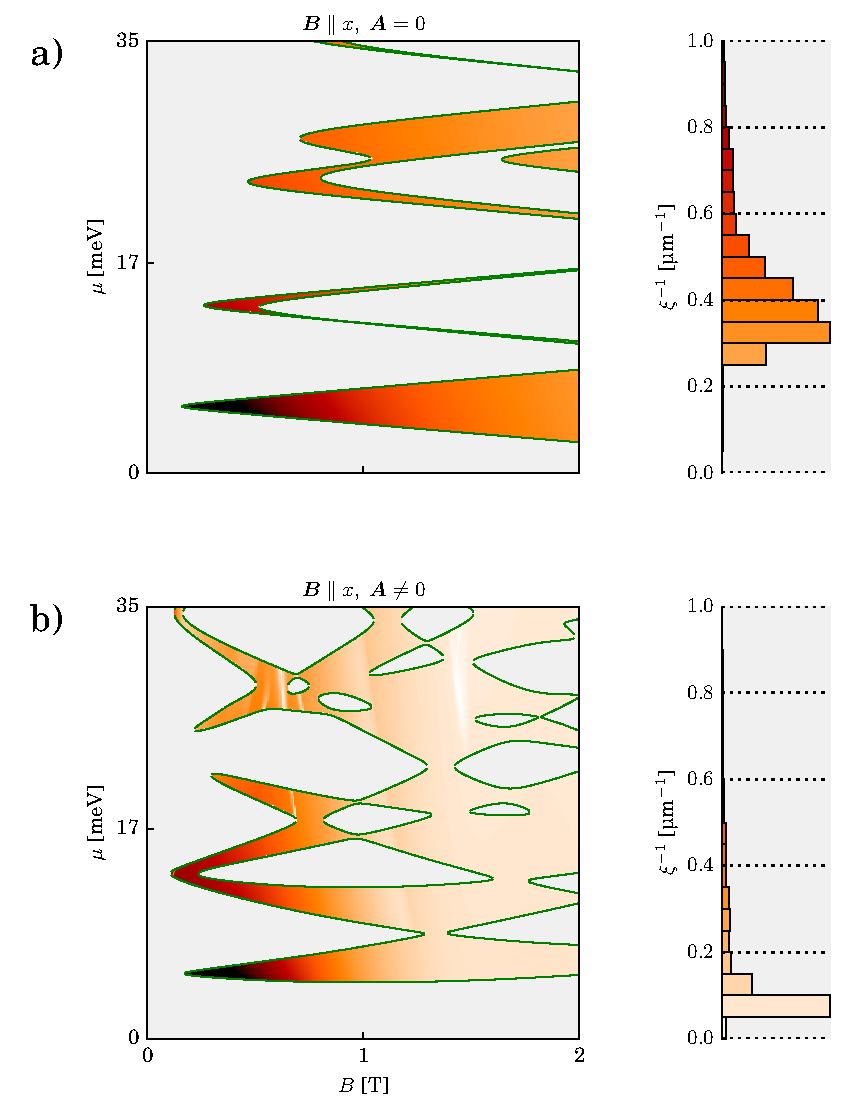
\includegraphics[width=0.95\columnwidth]{figures/sc_on_side_length}
\caption{Same as Fig.~\ref{fig:phase-diagram-sc_on_side}, but with color representing inverse Majorana length $\xi^{-1}$.
The histogram and color scales are truncated from above at $\SI{1}{\per\micro\metre}$.
The mode of the distribution of $\xi^{-1}$ reduces from $\SI{0.35}{\per\micro\metre}$ to $\SI{0.10}{\per\micro\metre}$ upon taking the orbital effect into account.
Although the Majorana lengths are overall much larger with the orbital effect of the magnetic field, the minimal length is close to $\SI{200}{\nano\metre}$ in both cases.\label{fig:Majorana-length}}
\end{figure}

\section{Results}

% \comment{We find that for relevant experimental parameters~\cite{Mourik2012}, Zeeman field effect is weaker than orbital.}

We use realistic parameters of an InSb nanowire~\cite{Mourik2012}: $\alpha=\SI{20}{\milli\electronvolt \nano\metre}$, $m^{*}=0.015m_e$, $\Delta=\SI{0.250}{\milli\electronvolt}$, $d=\SI{100}{\nano\metre}$, and $g=50$.
At the high fields that are typically used in experiment ($B\apprge\SI{1}{\tesla}$), we find that the Zeeman effect of the magnetic field has a lower impact on the phase boundaries than the orbital effect of the magnetic field (see Fig.~\ref{fig:phase-diagrams}).
We verify that the band gap is protected by $\mathcal{C}'$ as long as $B_y = 0$, despite that the orbital effect of the magnetic field reduces $E_\textrm{gap}$.

In agreement with our expectations a finite $B_y \lesssim \SI{0.1}{\tesla}$ leads to the closing of the band gap (see Figs.~\ref{fig:bandstructure} and \ref{fig:misaligned}).
The maximum tolerable $B_y $ becomes smaller with increasing $\mu$.
The narrow regions with suppressed $E_\textrm{gap}$ visible in Figs.~\ref{fig:phase-diagrams}(c) and \ref{fig:phase-diagrams}(d) are the consequence of Dirac cones appearing in $(k_{x}, B)$-space and are protected by $\mathcal{C}'$.
Breaking $\mathcal{R}_y$ breaks $\mathcal{C}'$ and removes these Dirac cones.

% \comment{With the reflection symmetry the gap closes quickly for fields in $y$ and $z$.}

We now turn to study the system shown in Fig.~\ref{fig:geometry}(c) that has $\mathcal{C}'$ strongly broken and only $\mathcal{R}_x$ and $\mathcal{P}$ remaining.
Since the induced superconducting gap $\Delta_\textrm{ind}\approx \SI{250}{\micro\electronvolt}$ in Ref.~\onlinecite{Mourik2012} is much smaller than the $\mathrm{NbTiN}$ gap $\SI{2}{\milli\electronvolt}$, the system must be in the long junction limit, where $E_\textrm{Th} \ll \Delta$.
In the long junction limit the induced gap equals $\Delta_\textrm{ind}\approx\hbar T v_\textrm{F} / d$, where $T$ is the transparency of the tunnel barrier, and $v_\textrm{F}$ the Fermi velocity.
In the absence of the orbital effect of a magnetic field, this means that the Zeeman energy has to exceed $\Delta_\textrm{ind}$ and therefore the critical value of the magnetic field at which the gap closes strongly depends on $\mu$ as seen in Fig.~\ref{fig:phase-diagram-sc_on_side}(a).
With the orbital effect of the magnetic field flux, penetration through the quasiparticle trajectory changes the interference phases, which suppresses the induced gap and causes the topological phase transitions to occur at a value of $B$ corresponding to a single flux quantum penetrating the wire area [see Fig.~\ref{fig:phase-diagram-sc_on_side}(b)].

The Majorana decay lengths $\xi$ significantly increase when including the orbital effect of the magnetic field in the Hamiltonian (see Fig.~\ref{fig:Majorana-length}).
Specifically, the mode of the distribution of $\xi$ changes by a factor of $\sim 4$ in the parameter range we consider (see histograms in Fig.~\ref{fig:Majorana-length}).
However, the minimum values of $\xi$ without orbital effect and with it are both $\approx \SI{200}{\nano\metre}$.
Therefore, $\mu$ needs to be tuned with sub-\unit{meV} precision within the lowest band in order to create Majorana bound states with practically relevant parameters.

% \comment{Higher spin-orbit strength does not seem to matter.}
To investigate the effect of the spin-orbit coupling on the Majorana properties in the presence of an orbital field, we have repeated the calculations shown in Figs.~\ref{fig:phase-diagram-sc_on_side} and \ref{fig:Majorana-length} using a fivefold larger spin-orbit strength reported in Ref.~\onlinecite{Weperen2015}.
We find that the topological band gap increases overall and in particular the maximal gap grows from $\SI{0.14}{\milli\electronvolt}$ to $\SI{0.21}{\milli\electronvolt}$, while the minimal decay length remains almost the same.
Therefore, increasing spin-orbit strength has a positive but not very strong effect on the topological band gap.

\section{Discussion and Conclusions}

% \comment{Our results: orbital field makes everything harder}
We have shown that the orbital effect of a magnetic field complicates the creation of Majoranas in nanowires.
Orbital terms break the chiral symmetry $\mathcal{C}$ and prevent the appearance of Majoranas whenever the magnetic field is not aligned with the wire axis.
When the field does point along the $x$-axis, we find that the reflection symmetry $\mathcal{R}_x$ in combination with particle-hole symmetry $\mathcal{P}$ protects the band gap from closing everywhere in $(B,\mu)$-space, except at the topological phase boundaries.
At experimentally relevant values of magnetic field, the orbital effect has a stronger impact on the dispersion relation than the Zeeman effect.
Furthermore, the orbital effect suppresses $E_\textrm{gap}$ and increases $\xi$.
However, the maximum value of the $E_\textrm{gap}$ in the topologically nontrivial region does not change as drastically (from $\SI{0.21}{\milli\electronvolt}$ to $\SI{0.14}{\milli\electronvolt}$) and the minimal decay length changes even less (from $\SI{201}{\nano\metre}$ to $\SI{210}{\nano\metre}$).
The reflection symmetry $\mathcal{R}_x$ of the Hamiltonian that we consider is respected by any Rashba spin-orbit interaction.
Dresselhaus spin-orbit coupling breaks $\mathcal{R}_x$; however, it is expected to be weak in the nanowires.

% \comment{Extensions: we omit several physical effects.}
Our simulations can be made more complete by complementing them with self-consistent electrostatics and magnetic field screening by the superconductor.
An additional extension of our work is to go beyond the effective mass approximation and to use the $k \cdot p$ model.
A separate topic of study is the interplay between the orbital effect of the magnetic field and disorder.
We expect that the sensitivity to disorder will increase by taking the orbital effect of the magnetic field into account.

% \comment{Outlook: how to cope with the complications.}
Our results suggest that keeping the chemical potential low is required to obtain Majoranas with reasonable length and energy scales.
Furthermore, our findings reveal a complication in realizing more sophisticated Majorana setups, such as a T-junction required for braiding.
This is because of the requirement that the field should be aligned with the nanowire.
A possible strategy to reduce the undesirable orbital effect of the magnetic field is to use nanowires with smaller diameters at a cost of reduced electric field effect and increased disorder sensitivity.

% \references{dissertation}
\references{orbitalfield}

\chapter{Supercurrent interference in few-mode nanowire Josephson junctions}
\label{ch:supercurrent}

\blfootnote{This chapter has been previously published as
Kun Zuo, Vincent Mourik, Daniel B. Szombati, Bas Nijholt, David J. Van Woerkom, Attila Geresdi, Jun Chen, Viacheslav P. Ostroukh, Anton R. Akhmerov, Sebasti{\'e}n R. Plissard, Diana Car, Erik P. A. M. Bakkers, Dmitry I. Pikulin, Leo P. Kouwenhoven, and Sergey M. Frolov, \textit{Supercurrent interference in few-mode nanowire Josephson junctions}, \href{https://doi.org/10.1103/PhysRevLett.119.187704}{Phys. Rev. Lett.~\textbf{119}, 187704, (2017)}
}
\blfootnote{My contributions to this work include writing parts of the paper, implementing the numerical methods to calculate supercurrents, and performing the numerical simulations.}

%% Start the actual chapter on a new page.
\newpage
\noindent
\section{Introduction}

Semiconductor nanowires coupled to superconductors form a promising platform for generating and investigating Majorana bound states \cite{Kitaev2001,Oreg2010,Lutchyn2010,Mourik2012,Deng2016,Albrecht2016,Chen2017a}.
Josephson weak links based on nanowires may provide additional evidence for Majorana bound states, e.g.~through the fractional Josephson effect \cite{Wiedenmann2016,Bocquillon2016,Deacon2017}.
These weak links can also become elements of Majorana-based topological quantum circuits \cite{Hyart2013, Aasen2016, Karzig2017, Plugge2017}.
Previous work on semiconductor nanowire Josephson junctions demonstrated supercurrent transistors \cite{Doh2005}, transport through few channels \cite{Goffman2017}, a nonsinusoidal current-phase relationship \cite{Spanton2017}, nanowire superconducting quantum interference devices (SQUIDs) \cite{Dam2006,Szombati2016}, and gate-tunable superconducting quantum bits \cite{Lange2015,Larsen2015}.
Recent works reported Josephson effects at high magnetic fields, sufficient to generate unpaired Majorana bound states \cite{Szombati2016,Paajaste2015,Tiira2017,Gharavi2017}.

In this chapter we study the critical current as a function of the magnetic field and gate voltage in nanowire Josephson junctions tuned to the mesoscopic few-mode regime.
The junctions consist of InSb weak links and NbTiN superconductor contacts.
For magnetic fields parallel to the nanowire, we observe a strong suppression of the critical current at magnetic fields on the scale of $\SI{100}{mT}$.
When the magnetic field exceeds $\sim \SI{100}{mT}$, the critical current exhibits aperiodic local minima (nodes).
In contrast with supercurrent diffraction in large multimode junctions, the magnetic field nodes of the critical current are strongly tunable by the voltages on local electrostatic gates, and are not uniquely determined by the junction geometry and supercurrent density distribution.
To understand our data, we develop a numerical model of a quasiballistic few-mode nanowire of realistic geometry.
Our model includes the intrinsic spin-orbit effect, as well as the vector-potential and Zeeman effects of the external magnetic fields.
Based on the simulations, we conclude that quantum interference between supercurrents carried by different transverse modes is the dominant mechanism responsible for both the critical current suppression, and the gate-sensitive nodes in the critical current.

\begin{figure}
\begin{center}
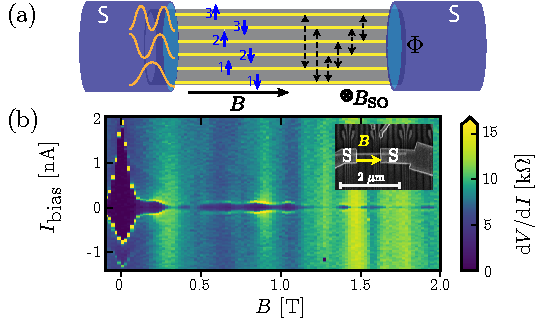
\includegraphics[width=0.7\columnwidth]{chapter_supercurrent/figures/fig1.pdf}
\caption{(a) Schematic superconductor ($S$)-nanowire-$S$ Josephson junction.
The cross section shows cartoon wave functions of $n=3$ transverse modes and the flux $\Phi$ penetrating the area of the nanowire.
The blue arrows indicate spin-resolved modes; the black dashed arrows are same-spin scattering events within the wire.
All modes are coupled at the contacts.
The directions of $B$ and the spin-orbit effective field $B_\mathrm{SO}$ are indicated.
(b) Differential resistance $\mathrm{d}V/\mathrm{d}I$ versus $B$ and $I_\mathrm{bias}$.
The current bias sweep direction is from negative to positive.
Data from device 1.
Inset: SEM image of a typical device similar to those studied here.
$S$ labels the superconducting contacts while $B$ indicates the in-plane magnetic field for device 2.}
\label{fig:figure1}
\end{center}
\end{figure}

\section{Experimental setup}
Figure \ref{fig:figure1}(a) presents a schematic of a few-mode nanowire Josephson junction.
The inset of Fig.~\ref{fig:figure1}(b) shows a device similar to those used in this study and their fabrication process is described in Ref.~\cite{Mourik2012}.
The junction consists of an InSb nanowire with a diameter of $100 \pm \SI{10}{nm}$ with 80 nm thick dc magnetron sputtered NbTiN contacts.
The wire sits on top of an array of 50 or $\SI{200}{nm}$ wide gates isolated from the junction by a dielectric.
We report data from devices 1 and 2 in the main text and show additional data from device 3 in the appendix.
Device 1(2) has a contact spacing of $\sim \SI{1}{\micro \m}$($\sim \SI{625}{nm}$) and the nanowire is at an angle of $25^\circ \pm 5^\circ$($0^\circ \pm 5^\circ$) with respect to $B$.
Device 3 has a shorter contact spacing of $\sim \SI{150}{nm}$ and shows similar behavior of gate-tunable nodes but the initial critical current decay is extended to 400 mT.
The measurements were performed in a dilution refrigerator with a base temperature of $\sim\SI{60}{mK}$.
All bias and measurement lines connected to the device are equipped with standard $RC$ and copper powder filtering at the mixing chamber stage to ensure a low electrical noise environment.
The voltage measurements are performed in the four-terminal geometry.

We set all the gates underneath the nanowire to positive voltages, in the few-mode transparent regime in which no quantum dots are formed between the superconducting contacts, and the normal state conductance exceeds $2e^2/h$ (see the full gate trace of the supercurrent in the appendix).

\section{Supercurrent measurements as a function of magnetic field}
Figure \ref{fig:figure1}(b) shows a typical example of the differential resistance $\mathrm{d}V/\mathrm{d}I$ as a function of the magnitude of the magnetic field $B$ and the current bias $I_\mathrm{bias}$ in this few-mode regime, with low resistance supercurrent regions in dark blue around zero current bias.
Note that the data at low field are asymmetric with respect to current reversal.
Only one sweep direction is plotted for the rest of the figures.

A strong decrease of the switching current is observed from $B=\SI{0}{T}$ to $B=100-\SI{200}{mT}$.
Beyond the initial decrease, the critical current exhibits nonmonotonic behavior with multiple nodes and lobes.
Despite the \SI{1}{\micro \meter} contact separation, the supercurrent can be resolved up to fields as high as $B=\SI{2}{T}$, which is comparable to the estimated strength of the effective spin-orbit field $B_\mathrm{SO}$.
At finite magnetic fields where the Josephson energy is suppressed the sharp switching behavior is replaced with a smooth transition to a higher resistance state.
In voltage-biased measurements, this manifests as a zero-bias conductance peak (see appendix).
This signal can mimic the onset of the topological phase since it is also associated with the zero-bias conductance peak that appears at a finite magnetic field.

\begin{figure}
\begin{center}
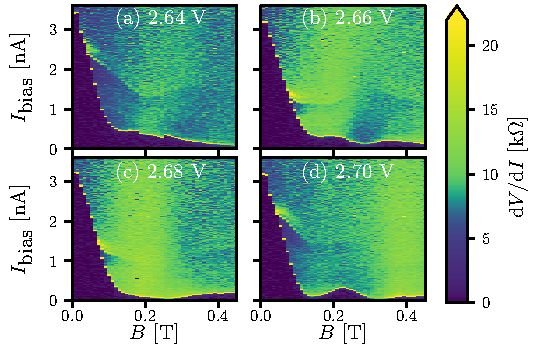
\includegraphics[width=0.7\columnwidth]{chapter_supercurrent/figures/fig2.pdf}
\caption{(a)-(d) $\mathrm{d}V/\mathrm{d}I$ vs $B$ and $I_\mathrm{bias}$ for different gate voltage settings $V_\mathrm{g}$ indicated above each panel.
Data from device 2; see the appendix for the scanning electron micrograph of the device with the tuned gate marked.}
\label{fig:figure2}
\end{center}
\end{figure}

\section{Possible mechanisms causing supercurrent oscillations}
We now qualitatively discuss the possible explanations for the behavior observed in Fig.~\ref{fig:figure1}(b).
Zeeman splitting can induce $0-\pi$-junction transitions which result in an oscillatory Josephson energy as a function of the magnetic field \cite{Bulaevskii1977,  Buzdin1982, Demler1997}.
This alternating $0-\pi$ junction behavior is due to spin-up and spin-down channels acquiring different phases as they travel across the junction [Fig.~\ref{fig:figure1}(a)].
However, in our junctions a strong spin-orbit effective field, which has been reported to point perpendicular to the nanowire \cite{Nadj-Perge2012}, reduces the relative phase shifts of spin-up and spin-down and lifts the nodes in the supercurrent \cite{Michelsen2008,Yokoyama2014,Yokoyama2014a}.
For the spin-orbit strength previously reported in InSb nanowires \cite{Nadj-Perge2012,Weperen2015}, we estimate an effective spin-orbit field $B_{\rm SO} \sim 1-\SI{2}{T}$ for a chemical potential value in the middle of the subband.
Therefore, we do not expect the occurrence of $0-\pi$-transitions in ballistic nanowires for fields much lower than this typical value of $B_{\rm SO}$, unless the chemical potential is close to a transverse mode edge (within $1-\SI{2}{meV}$), where $B_{\rm SO}$ is suppressed.
Given the typical mode spacing of $10-\SI{20}{meV}$~\cite{Weperen2012,Kammhuber2016}, in combination with the occurrence of several nodes well below \SI{1}{T}, the Zeeman $\pi$-junction effect is an unlikely explanation for all of the critical current nodes observed here for generic device settings.

Supercurrents carried by different transverse modes would also acquire different phase shifts and interfere due to mode mixing within the wire or at the contact between the nanowire and the superconductor lead~\cite{Gharavi2015}.
Such an interference is analogous to the Fraunhofer effect in wide uniform junctions: it becomes relevant when a single superconducting flux quantum is threaded through the nanowire cross section, a regime that is reached for $B \approx \SI{0.25}{T}$, well within the range of the present study.
A comparison of the experimental and numerical data in this chapter suggests that this is the effect that dominates the magnetic field dependence of the critical current.

Transitions in and out of the topological superconducting phase in the nanowire segments covered by the superconductors were also predicted to induce reentrant critical current\cite{San-Jose2014}.
Although we used devices similar to those presented in recent Majorana experiments \cite{Mourik2012,Guel2018,Chen2017a}, here we did not gate tune the regions of the wire underneath the superconducting contacts into the topological regime.
An accidental topological regime occurring on both sides of the junction in multiple devices is an unlikely explanation for the generic observations reported here.

\section{Supercurrent evolution with magnetic field and gate potential}
Figure~\ref{fig:figure2} shows a typical sequence of magnetic field dependences of the critical current, obtained by adjusting one of the narrow local gates.
The critical current exhibits multiple nodes [Fig.~\ref{fig:figure2}(d)], just a single node [Fig.~\ref{fig:figure2}(c)], or no node [Fig.~\ref{fig:figure2}(a)] in the same field range.
At some nodes the critical current goes to zero, while a nonzero supercurrent is observed at other nodes.
No periodic patterns such as those characteristic of a dc-SQUID or a uniform junction are observed.
Note that slight changes in the gate voltage are sufficient to dramatically alter the magnetic field evolution curve; the corresponding change in chemical potential $\Delta \mu$ is small ($\Delta \mu < \SI{1}{\milli \electronvolt}$) compared with the typical intermode spacing ($\sim \SI{15}{\milli \electronvolt}$).
Furthermore, the gate used only tunes a \SI{100}{\nano \meter} segment of the \SI{650}{\nano \meter} long junction.

Typical gate sweeps of the supercurrent are presented in Fig.~\ref{fig:figure3}.
The critical current is strongly reduced at fields above \SI{100}{\milli \tesla} irrespective of the gate voltage.
At all fields, the supercurrent is strongly modulated by the gate voltage.
However, gate voltages at which nodes in the critical current occur differ for each magnetic field.
Thus, no straightforward connection can be made between the zero-field critical current and node positions at a finite field, see also Fig.~\ref{fig:figure5}(a).

\begin{figure}
\begin{center}
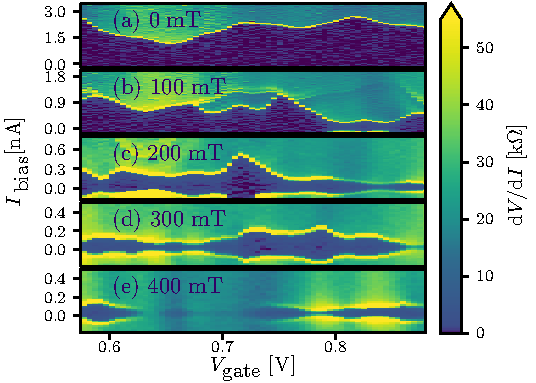
\includegraphics[width=0.7\columnwidth]{chapter_supercurrent/figures/fig3.pdf}
\caption{(a)-(e) $\mathrm{d}V/\mathrm{d}I$ vs $V_\mathrm{g}$ and $I_\mathrm{bias}$ at different $B$ (indicated within each panel).
Data from device 2.
The gate used for tuning is different from that used in Fig.~\ref{fig:figure2}, see the appendix.
\label{fig:figure3}}
\end{center}
\end{figure}

\begin{figure}
\begin{center}
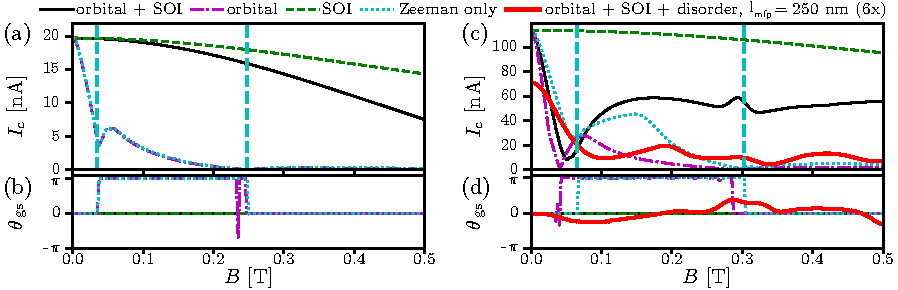
\includegraphics[width=\columnwidth]{chapter_supercurrent/figures/fig4.pdf}
\caption{Critical current and corresponding ground state phase difference for different combinations of terms in the Hamiltonian.
The Zeeman effect ($g=50$) is present in all of the curves.
Only the system corresponding to the red curve labeled with $l_\textrm{mfp}=\SI{250}{nm}$ includes disorder, for which the critical current is multiplied by a factor of 6.
The simulation is performed at $T=\SI{100}{mK}$.
The curves in panels (a) and (b) are for a single spinful transverse mode ($\mu=\SI{10}{meV}$).
Panels (c) and (d) are for the multimode (three transverse or six spin-full modes) regime ($\mu=\SI{20}{meV}$).
The vertical thick dashed light blue lines in (a) and (c) indicate the positions of $0-\pi$ transitions in the absence of disorder and with $\alpha = 0$, $\mathbf{A}=0$.
Where not specified, the other constant simulation parameters are $\alpha=\SI{20}{\nm \meV}$, $m_\textrm{eff}=0.015 m_\textrm{e}$, $\Delta_\textrm{ind}=\SI{0.250}{meV}$; the lattice constant $a=\SI{8}{nm}$, the nanowire diameter $d_1=\SI{104}{nm}$, the outer diameter (with superconductor) $d_2=\SI{120}{nm}$, and the superconductor coverage angle $\phi=135\si{\degree}$.
For plots of corresponding current-phase relationships, Josephson energies, and numerical geometry, see the Fig.~\ref{fig:system},~\ref{fig:currents_1D_alpha_vs_B_x}, and~\ref{fig:CPR}.
}
\label{fig:critical_currents}
\end{center}
\end{figure}

\section{Theoretical model}
In order to understand the magnetic field evolution of the Josephson effect, we develop an effective low-energy model of a spin-orbit and Zeeman-coupled few-mode nanowire, covered by superconductors at both ends.
We define $x$ as the direction along the wire, $y$ perpendicular to the wire in the plane of the substrate, and $z$ perpendicular to both wire and substrate.
The corresponding Hamiltonian reads
\begin{align}
H = &\left(\frac{\mathbf{p}^2}{2m^*}-\mu + \delta U\right)\tau_z + \alpha (p_x \sigma_y - p_y \sigma_x)\tau_z \nonumber \\ &+ g \mu_B \mathbf{B}\cdot\boldsymbol{\sigma} + \Delta \tau_x.
\label{eq:H}
\end{align}
Here $\mathbf{p}=-i\hbar\nabla+e\mathbf{A}\tau_z$  is the canonical momentum,  where $e$ is the electron charge, and $\mathbf{A}={\left[ B_y z - B_z y,\; 0,\; B_x y\right]}^{T}$ is the vector potential chosen such that it does not depend on $x$.
Further, $m^*$ is the effective mass, $\mu$ is the chemical potential controlling the number of occupied subbands in the wire, $\alpha$ is the strength of Rashba spin-orbit interaction, $g$ is the Land{\'e} $g$-factor, $\mu_\mathrm{B}$ is the Bohr magneton, and $\Delta$ is the superconducting pairing potential.
The Pauli matrices $\sigma_i$ and $\tau_i$ act in spin and electron-hole spaces, respectively.
We assume that the electric field generated by the substrate points along the $z$ direction, such that the Rashba spin orbit acts in the $xy$\kern-.05ex-plane, which is at low energies equivalent to an effective magnetic field $\mathbf{B}_{\rm SO}\parallel\hat{y}$.
We include the vector potential in the tight-binding system using the Peierls substitution \cite{Hofstadter1976}.
Finally, we include an uncorrelated on-site disorder $\delta U \in [-U, U]$, with $U$ the disorder strength, which we parametrize by a normal state mean free path $l_\textrm{mfp}$~\cite{Beenakker1997}.\footnote{To determine $l_\textrm{mfp}$ we calculate a disorder-averaged normal state conductance $g$ and evaluate the mean free path $l_{mfp}$ by fitting, $g=g_0 N_\textrm{ch} / (1 + L / l_\textrm{mfp})$, with $N_\textrm{ch}$ the number of conduction channels, and $g_0$ conductance quantum.}

We perform numerical simulations of the Hamiltonian \eqref{eq:H} on a 3D lattice in a realistic nanowire Josephson junction geometry.
The critical current is calculated using the algorithm described in Ref.~\cite{Ostroukh2016} and the Kwant code \cite{Groth2014}.
We note that for moderately damped and overdamped Josephson junctions, such as those studied here, the theoretical $I_c$ closely follows the experimentally measured switching current \cite{Kautz1990}.
The source code and the specific parameter values are available in the appendix.
The full set of materials, including computed raw data and experimental data, is available in Ref.~\cite{Zuo2017}.

\section{Discussion}
Numerical results are presented in Figs.~\ref{fig:critical_currents} and \ref{fig:figure5}(b).
First, we discuss the case of only a single transverse mode occupied [Figs.~\ref{fig:critical_currents}(a) and ~\ref{fig:critical_currents}(b)], which is pedagogical but does not correspond to the experimental regime.
When all field-related terms of Eq.~\eqref{eq:H} are included ($\mathbf{A}\neq 0$, $\alpha \neq 0$), we observe a monotonic decay of the critical current much more gradual than in the experiment, due to the absence of the intermode interference effect in the single-mode regime.
The $\pi$-junction transitions do not appear up to fields of order $\SI{0.5}{T}$ due to the strong spin-orbit effective field, which keeps spin-up and spin-down at the same energy so that they acquire the same phase shifts traversing the junction.
The critical current eventually decays because the Zeeman term overtakes the spin-orbit term at fields greater than \SI{0.5}{\tesla}.
When the spin-orbit term is turned off ($\alpha = 0$), we see several $0-\pi$ transitions taking place within the studied field range, confirmed by the ground state phase switching between 0 and $\pi$ at a series of magnetic fields [Fig.~\ref{fig:critical_currents}(b)].

The experimentally relevant regime is when several transverse modes are occupied.
The measurements display three qualitative features: (i) the initial critical current at $B=\SI{0}{T}$ is strongly suppressed within $100-200$mT; (ii) the critical current then revives and continues to display nodes of variable depth and periodicity; (iii) this revival of the critical current after suppression is about 10\% of its original value at $B=\SI{0}{T}$.
Models that neglect the orbital effect display either a slow monotonic decay of the critical current (spin-orbit included, $\alpha \neq 0$), or regular critical current nodes due to $0-\pi$ transitions (no spin-orbit, $\alpha=0$) [Fig.~\ref{fig:critical_currents}(d)], as in the single-mode case.
When orbital effects are included, $\mathbf{A}\neq 0$, observations (i) and (ii) are reproduced but the revival of the critical current after initial suppression is still strong.
Inclusion of a realistic amount of disorder, which creates additional interference paths and suppresses supercurrent further, reproduces all observations (i), (ii), and (iii).
Thus, we conclude that the experiment is best reproduced when $\mathbf{A}\neq 0, \alpha \neq 0$ and weak disorder that induces intermode scattering is included within the junction model.

The inclusion of disorder in the multimode regime breaks mirror symmetry~\cite{Yokoyama2014,Yokoyama2014a} and generates a spin-orbit field along the external magnetic field \textit{B}, which gives rise to a nonsymmetric current-phase relation, inducing a $\varphi_0$ junction (see Sec.~\ref{sec:cpr_jj_energies} for a detailed explanation).
The ground state phase of the $\varphi_0$ junction can continuously change between 0 and $\pi$ [red trace in Fig.~\ref{fig:critical_currents}(d)].
Experimental verification of such phase-related effects is not possible in the two-terminal junction geometry used here, it requires phase-sensitive experiments in the SQUID geometry.

\begin{figure}
\begin{center}
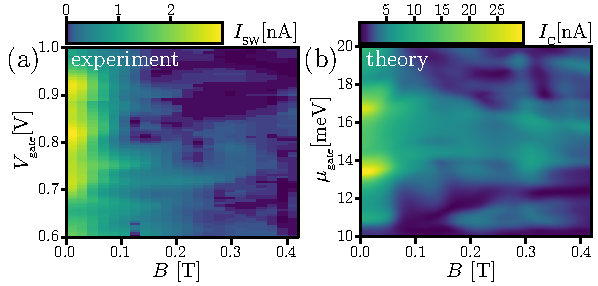
\includegraphics[width=0.7\columnwidth]{chapter_supercurrent/figures/fig5.pdf}
\caption{Comparison between experimental (a) and numerical (b) results.
The parameters for the numerical simulations are the same as in Figs.~\ref{fig:critical_currents}(c) and \ref{fig:critical_currents}(d), red curve.
The range of the chemical potential in the gated region ($\mu_{\textrm{gate}}$) is chosen using Ref.~\cite{Vuik2016}.
The experimental data are taken with device 2.}
\label{fig:figure5}
\end{center}
\end{figure}

In Fig.~\ref{fig:figure5} we compare side-by-side experiment and simulations via field-versus-gate maps of the supercurrent.
In Fig.~\ref{fig:figure5}(a), the switching current from a set of $\mathrm{d}V/\mathrm{d}I$ versus $I_\textrm{bias}$ traces similar to those in Fig.~\ref{fig:figure3} was extracted from device 2 (see the appendix for algorithm details).
Beyond the decay of the switching current on the scale of $\SI{100}{mT}$, the experimental data show a complex evolution of switching current maxima and minima in gate-field space.
Characteristic features of this evolution are reproduced by our simulation shown in Fig.~\ref{fig:figure5}(b).
In particular, the experimentally observed magnetic field scale of initial supercurrent decay is reproduced in the simulation.
Furthermore, the gate-tunable maxima and minima of the critical current are recovered in our model; both in experiment and simulation these do not evolve in a regular fashion (a consequence of the complexly shaped interference trajectories).
This qualitative agreement found additionally substantiates the applicability of our model to the experimental results.

\section{Conclusions}
Our results are instrumental for modeling Majorana setups.
Specifically, the decrease of Josephson energy by an order of magnitude is observed at fields at which the onset of topological superconductivity is reported.
This effect should, therefore, be taken into account in efforts to realize recent proposals for fusion and braiding of Majorana fermions \cite{Hyart2013,Aasen2016,Plugge2017,Karzig2017}, especially in those that rely on controlling the Josephson coupling \cite{Hyart2013,Aasen2016,Plugge2017}.
Our findings are applicable not only to bottom-up grown nanowires and networks but also to scalable few-mode junctions fabricated out of two-dimensional electron gases~\cite{Nichele2017,Lee2019}.
We suggest that in such devices narrow multimode nanowires should be used.
At the magnetic field strengths required for braiding the many modes would facilitate strong Josephson coupling, whereas a small diameter prevents its suppression due to supercurrent interference.

Phase-sensitive measurements in the SQUID loop geometry will reveal effects  such as the Zeeman-induced  $\pi$ junction and the spin-orbit induced $\varphi_0$ junction, which our study identifies numerically but does not access experimentally.
Single quantum mode junctions are within reach thanks to the recent demonstration of quantum point contacts in InSb nanowires at a zero magnetic field \cite{Kammhuber2016}.
In that regime phenomena such as induced $p$-wave superconductivity can be studied in a unique gate-tunable setup, when tuning down to a single spin-polarized mode in the weak link.
The results are also applicable to other interesting material systems where spin-orbit, orbital,  and Zeeman effects interplay - systems such as Ge/Si, PbS, InAs, and  Bi nanowires and carbon nanotubes~\cite{Cleuziou2006}.

\section{Appendix}\label{sec:appendix_supercurrent}

\subsection{Zero field gate dependence}

\begin{figure}
\begin{center}
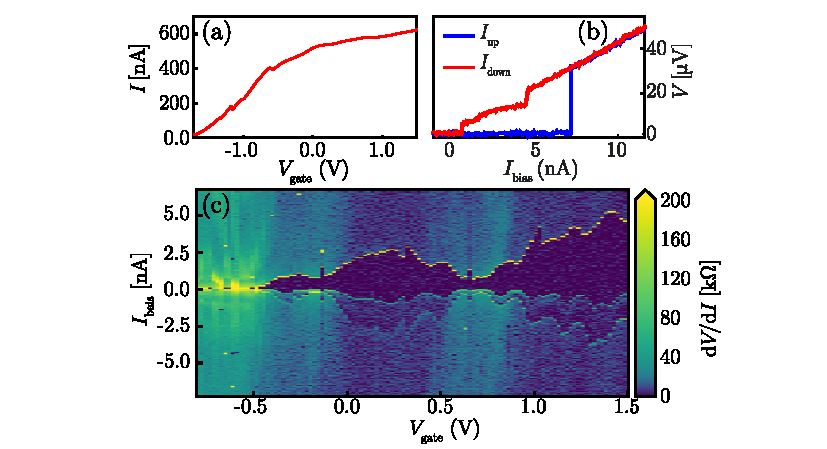
\includegraphics[width=\columnwidth]{chapter_supercurrent/figures/sup_fig1.pdf}
\caption{(a) Device current as a function of gate voltage, $V_\mathrm{bias}$ = 10 mV.
Except the gate that is varied in this scan, other gates are at +3 V.
(b) Voltage-current characteristic for both upwards (blue) and downwards (red) sweeping direction of current bias.
The supercurrent of 8 nA is the maximum supercurrent observed in this device and corresponds to all gates at +3V.
(c) Numerical derivative $\mathrm{d}V/\mathrm{d}I$ of $V\left(I\right)$ as function of current and gate voltage.
Current bias is swept from negative to positive.}
\label{fig:charaterization_D1}
\end{center}
\end{figure}

Characterization of device 2 at $B$=0 T is shown in Fig.~\ref{fig:charaterization_D1}, devices 1 and 3 behave similarly (data not shown).
Current versus local gate voltage is measured at $V_{\text{bias}}$ = 10 mV (Figure \ref{fig:charaterization_D1}(a)).
Taking known series resistances into account, the device resistance of $\sim$6 k$\Omega$ is found, corresponding to the sum of the conduction channels and contact resistances.

As shown in Fig.~\ref{fig:charaterization_D1}(b), by optimizing the gate voltages a maximal supercurrent of 8 nA was found, with a corresponding voltage of 32 $\mu$V, which developed upon switching to the normal state.
The junction is hysteretic as shown by the low retrapping current, and has a sharp transition to the normal state, indicating that the junction is in the underdamped regime.
Note that self-heating may also contribute to the hysteresis \cite{Courtois2008}.

\subsection{Shapiro step measurements}

\begin{figure}
\begin{center}
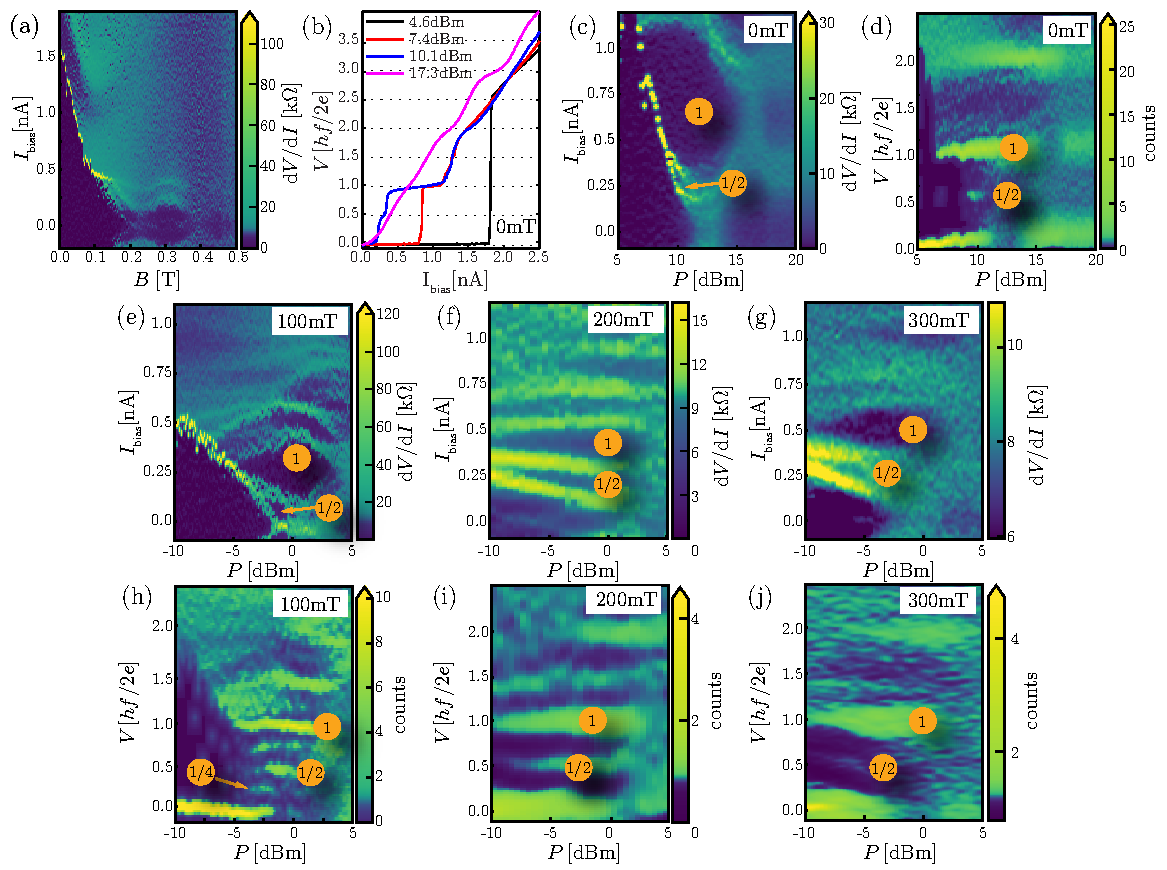
\includegraphics[width=\columnwidth]{chapter_supercurrent/figures/sup_fig2}
\caption{
Shapiro steps in magnetic field.
(a) $B$ dependence of supercurrent without microwave radiation applied.
Numerical derivative $\mathrm{d}V/\mathrm{d}{I}$ of the original $V\left(I\right)$ curves is shown.
(b) Shapiro steps at $B = \SI{0}{\tesla}$ for different microwave powers.
At the lowest RF power of 4.6 dBm (black line) no Shapiro steps are present.
A half integer step is visible at 10.1 dBm (blue line).
(c),(e)-(g) Microwave power dependence of Shapiro steps for different $B$.
Numerical derivative $\mathrm{d}V/\mathrm{d}{I}$ of the original $V\left(I\right)$ curves is shown, in this representation the Shapiro step plateau corresponds to low differential resistance (blue color).
(d), (h)-(j) are Shapiro steps for different $B$ as a function of microwave power plotted in histogram.
High voltage counts correspond to the plateaus in the Shapiro steps.
At $B = \SI{0}{\tesla}$ [panel (c)], the power dependence is dominated by integer Shapiro steps and only a small contribution of half integer steps is visible.
At $B = \SI{100}{m\tesla}$ [panel (e)]  fractional steps are visible.
Noticeably, not only half integer steps, but also quarter steps are weakly present in panel (h).
$B = \SI{200}{m\tesla}$ [panel (f)] is closest to the minimum supercurrent at \SI{250}{m\tesla}.
Here the half integer and integer steps are almost equal in width.
Finally, beyond the minimum of supercurrent, at $B = \SI{300}{m\tesla}$ [panel (g)], the integer steps increase again in width relative to the half integer step.
Curves in (b) are from the same dataset as shown in (c).
Values given for the RF power in panels (b)-(j) are the output power of microwave source, \SI{60}{\deci \bel} attenuation, of which \SI{20}{\deci \bel} at low T, is applied.
Data is from device 2, second cooldown.}
\label{fig:shapiro}
\end{center}
\end{figure}

Device 2 has been cooled down a second time with a microwave antenna near the sample.
This enabled the study of Shapiro steps in the junction as a function of microwave power and frequency, see Fig.~\ref{fig:shapiro}.
The device is again tuned to a multi-mode regime, comparable to $V_\mathrm{gate}$ = 0.5 V in Fig.~\ref{fig:charaterization_D1}(c).
Due to an increased microwave background noise in the vicinity of the junction upon adding the antenna, an extra rounding of the $V\left(I\right)$-trace near the switching bias is present.

Figure \ref{fig:shapiro}(a) is a magnetic field $B$ dependence of supercurrent in the absence of microwave drive.
The supercurrent pattern as a function of $B$ is similar to the one shown in Fig.~\ref{fig:figure2}.
This indicates that thermally cycling the device did not change the qualitative behavior of the device, although the exact gate tunings are different.

We focus on the power dependence of Shapiro steps at different $B$ strengths of 0mT, 100mT, 200mT and 300 mT corresponding to Fig.~\ref{fig:shapiro}(c), (e), (f), (g) respectively.
The microwave frequency is kept fixed at 2.0 GHz.
Shapiro steps show up at voltages corresponding to $V=n\cdot\frac{hf}{2e}$, where $n$ may be a fraction.
At $B$ = 0 mT [Fig.~\ref{fig:shapiro}(c)], half integer steps are only weakly present.
At $B$ = 100 mT [Fig.~\ref{fig:shapiro}(e)], not only $n$ = 1/2 steps but also weak $n$ = 1/4 steps are visible (not marked with circled number).
This is clearly visible in Fig.~\ref{fig:shapiro}(h), where the same data is plotted in a voltage histogram, with high voltage counts corresponding to the plateaus of the Shapiro steps.

The $B$ = 200 mT and $B$ = 300 mT cases [Fig.~\ref{fig:shapiro}(f), (g)] correspond to low critical currents.
Nevertheless, Shapiro steps can still be resolved.
At B = 200 mT, which is closest to the minimum of critical current, the width of the 1/2 step is more than half the width of the 1st step, and it is similarly large compared to the 1st step at 300 mT.
Fig.~\ref{fig:shapiro}(i), (j) are the histogram representations of Fig.~\ref{fig:shapiro}(f), (g).

Shapiro steps at fractional frequencies, especially the half-integer steps, have been previously observed in Josephson junctions under various conditions\cite{Lehnert1999,Dubos2001, Dinsmore2008,Sellier2004,Chauvin2006}.
For instance, they can arise due to Josephson coupling of higher orders accompanied by a non-sinusoidal current-phase relationship\cite{Radovic2001}.
In quasi-ballistic few-mode Josephson junctions the current-phase relation is expected to be non-sinusoidal, consistent with half-integer Shapiro steps observed here even at zero magnetic field.
The higher order 1/4-steps are more exotic and deserve a deeper study in the future, though they may also originate from a non-sinusoidal current-phase relationship.
Non-sinusoidal current-phase relationships are obtained within our model, see Fig.~\ref{fig:CPR}.
However, Fourier analysis of the simulation suggests that Shapiro steps at 1/3 the Josephson voltage should dominate over 1/4 steps.
This discrepancy remains not understood.

In a non-sinusoidal Josephson junction tuned to the $0-\pi$ transition the first order Josephson effect which is responsible for strong integer Shapiro steps vanishes, thus the current phase relationship is dominated by higher harmonics.
In this case, Shapiro steps at half-integer and integer frequencies are expected to appear with the same step widths.
The results presented here show that the ratio of step widths for half integer to integer steps indeed increases near a field-induced node in the critical current.
However, the results are not conclusive as to whether this is due to a $0-\pi$ transition.

On the other hand, Majorana zero modes coupled across a junction barrier are predicted to result in disappearing odd-integer Shapiro steps\cite{Lutchyn2010,Oreg2010}.
Thus the behavior observed here is opposite to that expected due to Majorana modes: extra fractional steps in addition to integer steps are observed.

\subsection{Angle dependence of fluctuations}

In this section we present results from device 3 [Fig.~\ref{fig:SEM_D1D3}(c)] with contact spacing of 150 nm on which we performed current bias measurements with similar conditions as reported in the main text.
Device 3 is fabricated with similar methods as device 1 and 2, with the exception that $\text{HfO}_x$ is used as the dielectric material instead of $\text{SiN}_x$.

\begin{figure}
\begin{center}
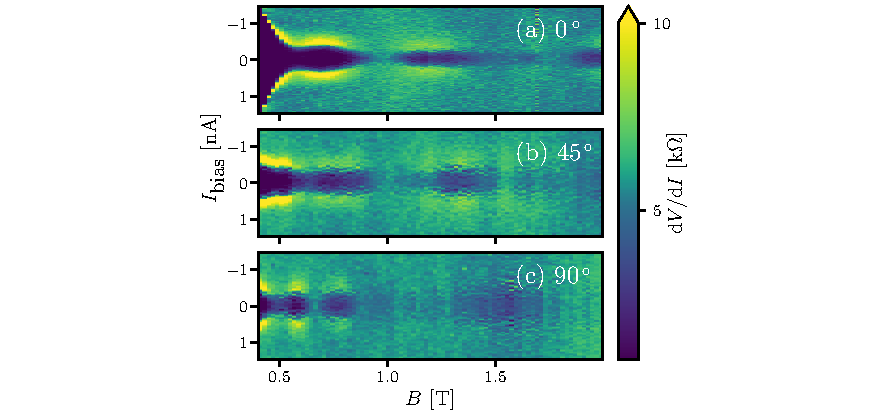
\includegraphics[width=\columnwidth]{chapter_supercurrent/figures/sup_fig3}
\caption{Differential resistance measured as a function of current bias and magnetic field strength of device 3.
The angle indicated in each panel is the angle of the magnetic field relative to the wire axis, in the plane of the substrate.}
\label{fig:angle_dependence}
\end{center}
\end{figure}

The device shows a monotonic decrease of the critical current for magnetic field values up to 400 mT (not shown in the figure).
This extended initial decay is attributed to the shorter contact separation, and hence reduced influence of disorder on intermode interference.

Beyond 400 mT, the critical current fluctuates at a period depending on the direction of the magnetic field.
Figure \ref{fig:angle_dependence} shows the differential resistance of the device for three different field directions.
The top panel shows data where the field is pointed along the nanowire.
The critical current decays until the field reaches 600 mT, beyond which it exhibits a weakly pronounced maximum and disappears at 900 mT after which it reappears again.
As the field angle is rotated in the plane of the substrate [Figs.~\ref{fig:angle_dependence}(b),(c)], the critical current decays faster as a function of the field strength, and the subsequent nodes of the critical current are closer spaced in field.
We associate this behavior with increased flux through the nanowire at finite angles between the field and the wire.

\begin{figure}
\begin{center}
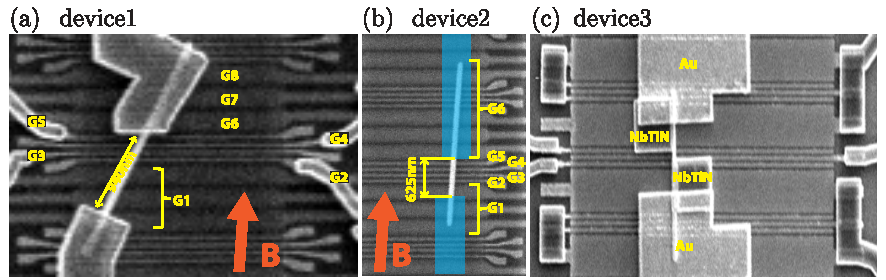
\includegraphics[width=\columnwidth]{chapter_supercurrent/figures/sup_fig4.pdf}
\caption{Schematics based on SEM picture of device 1, device 2 and device 3.
(a) Device 1, with an angle of $25^{\circ} \pm 5^{\circ}$ with the magnetic field.
In all devices, not all local gates are operated independently: as indicated in the figures, larger gates are formed by shorting some of the local gates together, e.g G1.
(b) Device 2, shown with the superconducting electrode design superimposed on top of the SEM image, as this device has not been imaged after the final fabrication step.
The device has a contact spacing of $\sim \SI{625}{nm}$, with the wire at an angle of $0^\circ \pm 5^\circ$ with respect to magnetic field.
(c) Device 3, incorporating two quasi-particles traps (Au) next to the superconducting contacts.
The length of the Josephson junction is $\sim \SI{150}{\nano \meter}$.
Device 3 is cooled down in a setup where the magnetic field could be rotated using a 3D vector magnet.}
\label{fig:SEM_D1D3}
\end{center}
\end{figure}

\subsection{Zero bias peaks due to supercurrent can onset at finite magnetic field}

If the Josephson junctions are tuned into the topological regime, devices used in this study can also support Majorana fermions.
As a matter of fact, such a design is employed by several groups for the purpose of searching for Majorana zero modes.
Here we show that such Josephson junction based devices, even if the contacts are almost \SI{1}{\micro \meter} apart, cannot be used for unambiguous detection of Majorana zero modes \cite{Deng2012, Deng2014, Finck2013}.
Specifically, we observe that, in a voltage-biased measurement, supercurrent can appear as a zero-bias peak that onsets at a finite magnetic field, in the same range of parameters as those used in Majorana experiments, thus mimicking a key Majorana signature.

Figure \ref{fig:supercurrentZBP} shows the results.
By applying a negative voltage to one of the local gates in between the superconducting contacts, a tunneling regime comparable to $V_\mathrm{gate}$ < -0.5 V shown in Fig.~\ref{fig:charaterization_D1}(a) for device 2 is achieved.
The result of a current biased measurement in this regime is shown in Fig.~\ref{fig:figure5}(a), a very small (down to 1 pA) supercurrent could be resolved.
Interestingly, for gate regimes with lower resistance the supercurrent initially grows as expected, but then the $\mathrm{d}V/\mathrm{d}I$ peak related to the switching current broadens and is no longer visible.
Here, we focus on the $B$ dependent behavior as shown in Fig.~\ref{fig:supercurrentZBP}(b),(c),(d) at a gate voltage indicated by the yellow line in Fig.~\ref{fig:supercurrentZBP}a.
At $B=\SI{0}{T}$, no supercurrent was resolved in a current biased measurement, but upon increase of magnetic field, at around 200 mT, a small supercurrent shows up in a slightly more resistive regime.
Such a small supercurrent may show up in a differential conductance measurement as a small zero bias peak (ZBP).
Indeed, upon switching to a voltage biased differential conductance measurement, a small ZBP with height $\sim 0.01\frac{2e^2}{h}$ is found.
Note that the ranges in which the supercurrent is visible in a current biased measurement and in which the ZBP is visible in a voltage biased measurement are not identical due to a minor charge switch between the two measurements.

\begin{figure}
\begin{center}
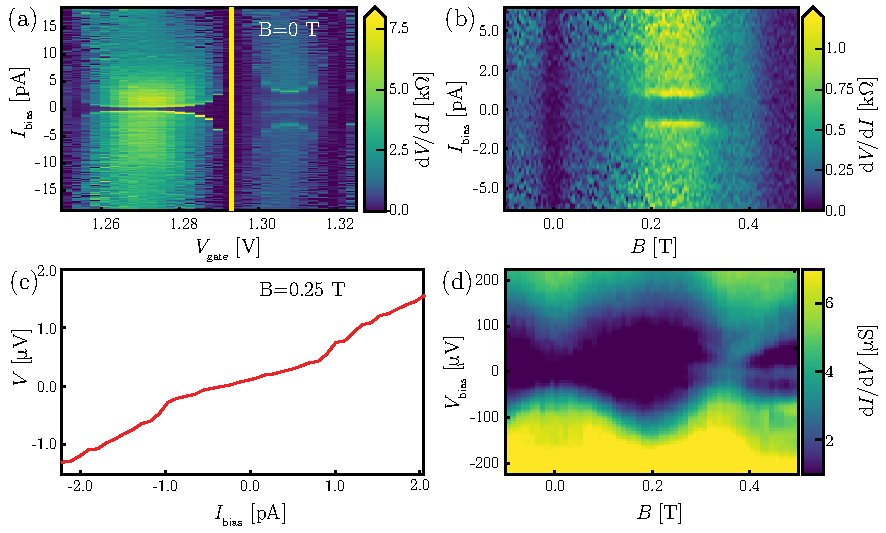
\includegraphics[width=\columnwidth]{chapter_supercurrent/figures/sup_fig5}
\caption{Supercurrents and zero bias peaks at finite $B$.
(a) Differential resistance vs gate.
In this scan, one of the local gates is set at -0.45 V and all other gates are at +1.5 V.
(b) Differential resistance vs $B$ at the indicated gate position in (a).
(c) Linecut from (b) at $B = \SI{0.25}{T}$.
(d) Differential conductance vs $B$ corresponding to (b).
Numerical derivative of original $V\left(I\right)$ curves is shown in (a) and (b).
Data from device 1.}
\label{fig:supercurrentZBP}
\end{center}
\end{figure}

\subsection{Extracting switching current from experimental data}

To obtain Fig.~\ref{fig:figure5}(a), switching currents are extracted from a large set of voltage-current characteristics by numerically detecting the voltage step upon switching from the superconducting to the resistive regime.
First, an initial low-pass filter is applied to the data reducing spurious fast fluctuations.
Next, a numerical derivative of the $V\left(I\right)$-curve is taken.
This first derivative has a clear maximum for an $V\left(I\right)$-curve with a sharp transition, allowing for straightforward identification of the switching current.
However, the finite $B$-field $V\left(I\right)$-curves typically display smooth transitions from the superconducting to the resistive state, resulting in unclear or even absent maximums in the first derivative.
A smooth transition still generates a maximum of the second derivative, allowing for identification of the switching current.
We, therefore, introduced a threshold for a first derivative maximum, below which a second derivative is taken of the $V\left(I\right)$-curve with its maximum identified as the switching current.
A second threshold is introduced for the maximum of the second derivative, below which the switching current is considered to be zero.
Algorithm parameters are optimized to both correctly identify the sharp transitions of large switching currents and to avoid false positives of small switching current.


\subsection{Details of the modeling}

We discretize the Hamiltonian Eq.~\eqref{eq:H} on a cubic lattice with a lattice constant of $a=\SI{8}{nm}$.
The nanowire cross section has a diameter of $\SI{104}{nm}$ and the superconductor on top of the semiconductor nanowire adds two more layers of unit cells partially covering the nanowire ($135^{\circ}$ of the wire's circumference).
There are 3 free parameters in the simulation for obtaining the correct induced gap in the nanowires, namely the coverage angle of the superconductor, the tunnel barrier between the SC and the SM, and the superconducting gap.
The coverage angle is fixed at $135^{\circ}$ in order to save computational time.
Since the Meissner effect is not included in the simulation, the exact value of the angle does not play a critical role.
The superconducting order parameter $\Delta$ is set such that the induced gap inside the nanowire at zero field is $\Delta_\textrm{ind} = \SI{0.250}{meV}$.

The superconductor has the same lattice constant and effective mass as the nanowire, justified by the long-junction limit.
This means that the wave function has most of its weight in the nanowire and that the superconducting shell merely serves as an effective boundary condition that ensures that all particles are Andreev-reflected.
Further, the superconductor lacks the Zeeman effect and spin-orbit interaction.
Zeeman effect in the superconductor is neglected because the g-factor in NbTiN is 2, much smaller than the g-factor in InSb (which is 50).
We use realistic parameters of an InSb nanowire~\cite{Mourik2012}:  $\alpha=\SI{20}{\meV\cdot\nm}$, $m^{*}=0.015 m_e$, and $g=50$.

The geometry of the modeled system is shown in Fig.~\ref{fig:system}.

\begin{figure}
\begin{center}
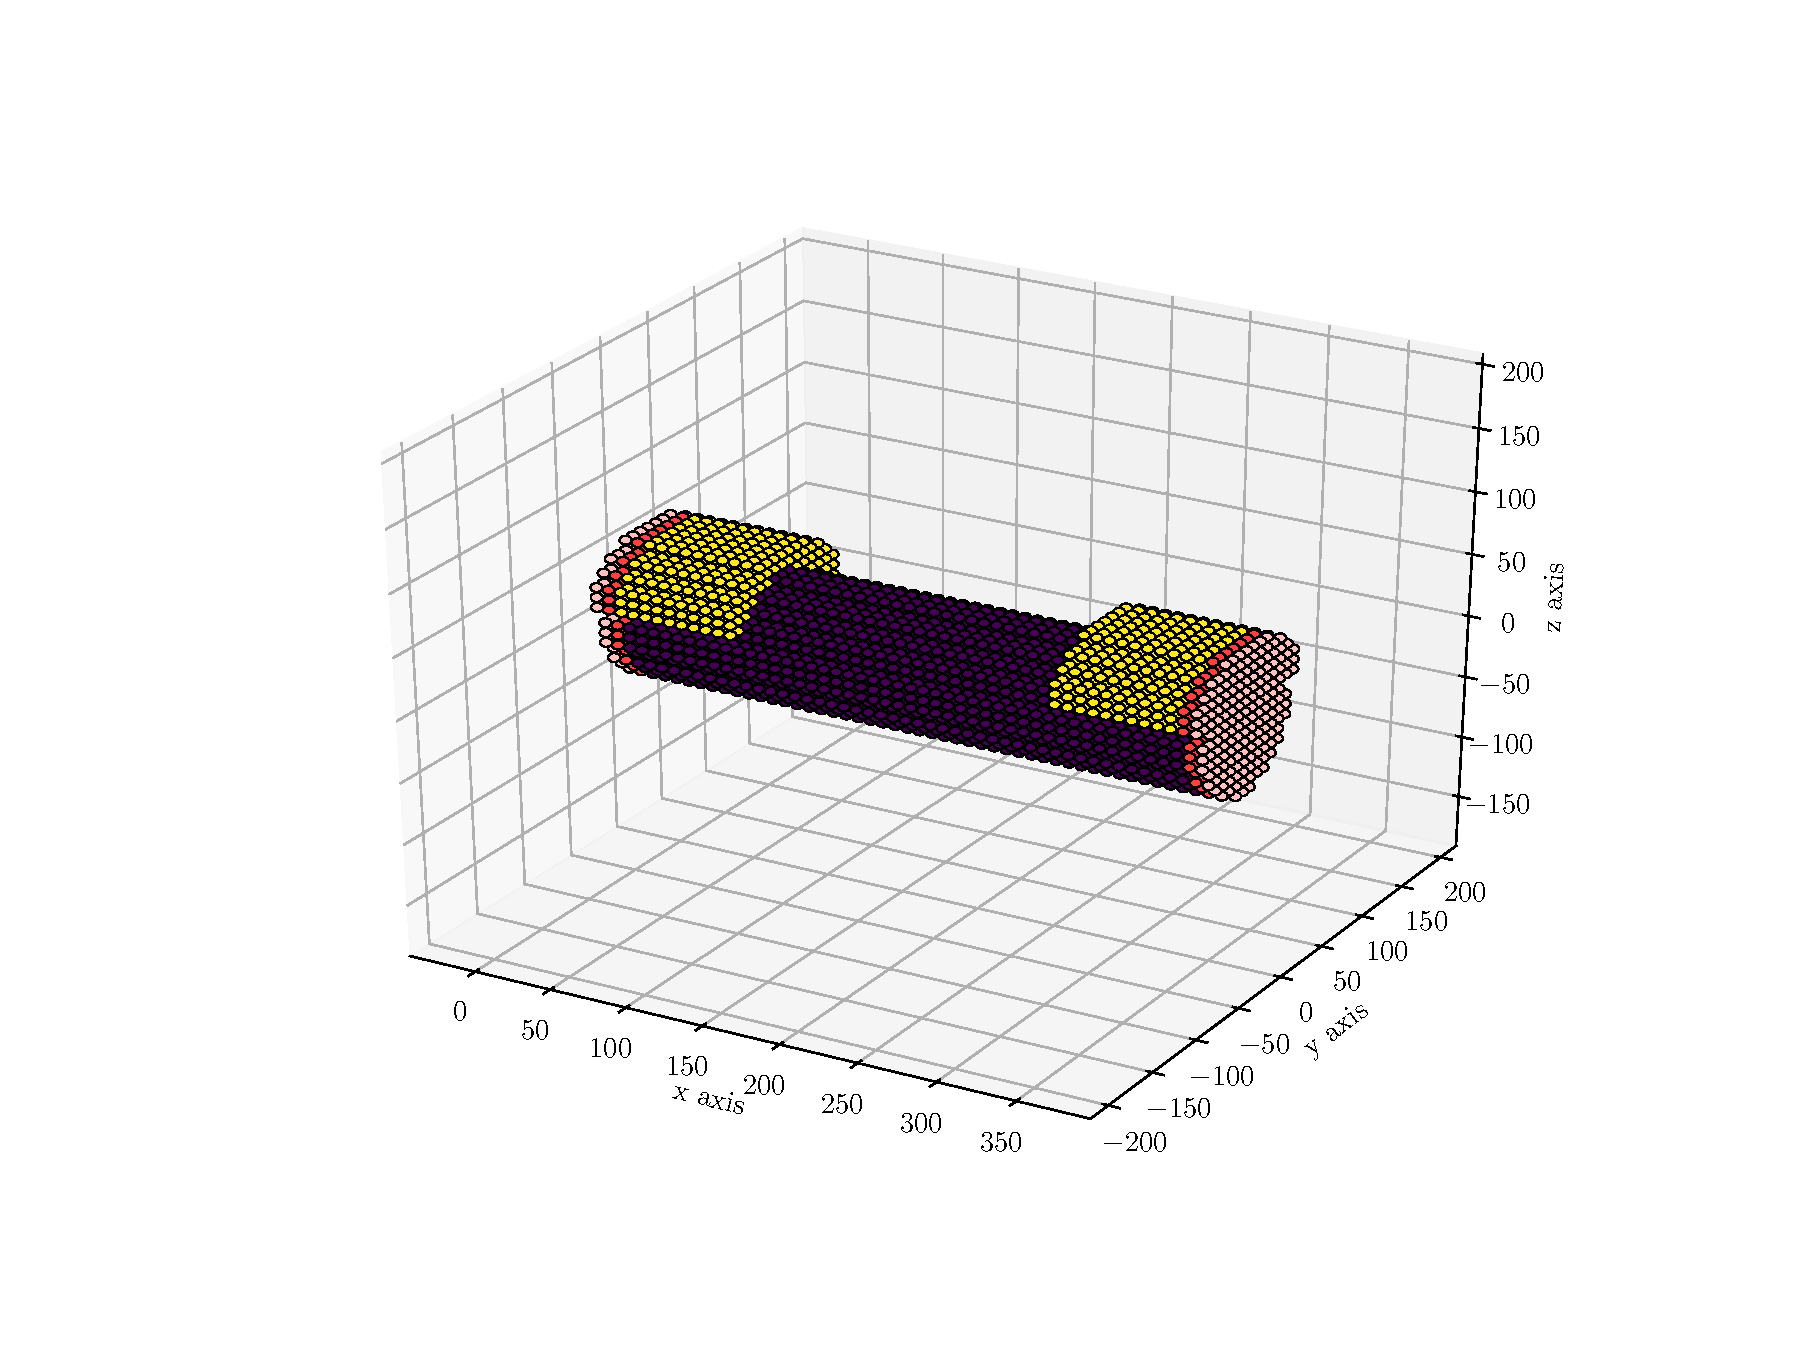
\includegraphics[width=\columnwidth]{chapter_supercurrent/figures/sup_fig6}
\caption{The modeled tight-binding system.
The purple sites indicate the semi-conductor and the yellow sites show the superconductor.
The red and light red colored cross sections indicate that the wire extends infinitely in that direction.
We defined the length of the wire $L$ as the part that is not covered with the superconductor.
In this figure for clarity we plot a shorter wire ($L=\SI{200}{\nm}$), while in the simulations we chose $L=\SI{640}{\nm}$.
The other dimensions used in the simulations are as depicted.
Specifically, the wire diameter is $\SI{104}{\nm}$, the thickness of the superconductor is $16-\SI{24}{\nm}$, and the coverage angle of the superconductor is 135$^{\circ}$.}
\label{fig:system}
\end{center}
\end{figure}

\subsection{Detailed theoretical estimates}
In this section we estimate the strength of different possible mechanisms that can cause supercurrent fluctuations in the nanowire Josephson junction.

\textit{Interference between orbital channels}.
The area of the cross section of the nanowire is $\sim \pi \times (\SI{50}{nm})^2$.
This means that the magnetic field value of $B \approx \SI{0.26}{T}$ corresponds to one flux quantum penetrating the cross section of the nanowire.
At this value of the magnetic field we expect the phase shifts between different bands propagating between the two superconductors to be comparable to $\pi$.
This sets the typical $B$ scale for the interference of different orbital modes carrying current, which is well within the experimentally observed typical difference in $B$ of consecutive critical current minimums.
This simple estimate neglects the magnetic field expulsion of the superconductor, which may create a higher flux in the nanowire near the superconducting contacts, thus lowering the effective field scale.

These estimates are similar to the analysis for the Fraunhofer-like interference in diffusive many-channel junctions\cite{Cuevas2007}.
The novelty is, however, in the small number of channels in our junction, which causes irregular interference instead of the regular Fraunhofer pattern in the former case.
Another important observation in our case is that even though the magnetic field is along the junction, it can still cause the interference due to different transverse profiles of the propagating modes.\\

\textit{Interference between spin channels}.
Supercurrent fluctuations can be produced by $0-\pi$ transitions due to the Zeeman splitting of the Andreev bound states inside the Josephson junction.
The characteristic $B$ scale of such supercurrent fluctuations is determined by the ratio of Zeeman energy to the Thouless energy.
This sets the relative phase $\theta_\mathrm{B}$ of the Andreev bound states, $\theta_\mathrm{B} = E_\mathrm{Z} L / \hbar v_\mathrm{F}$.
Here $E_\mathrm{Z}$ is the Zeeman energy, $L$ the length of the nanowire junction, and $v_\mathrm{F}$ the Fermi velocity in the nanowire.
The junction undergoes a $0-\pi$ transition when the relative phase difference of the ABS $\theta_\mathrm{B}$ reaches the value $\pi/2$.
Such a transition is marked by a minimum in the junction critical current as a function of $B$.
Since $v_\mathrm{F}\approx \sqrt{2\mu / m^*}$, the field value at which $\theta_\mathrm{B}=\pi/2$ depends on the chemical potential $\mu$.
We thus estimate the upper bound of the magnetic field at which the first $0-\pi$ transition occurs by assuming a maximal value of $\mu \sim \SI{15}{meV}$ corresponding to the intermode spacing\cite{Weperen2015,Kammhuber2016}.
Assuming a junction length of $L=\SI{1}{\micro\meter}$, the upper bound of the transition occurs at $B\sim \SI{0.5}{T}$.
Generally, for smaller $\mu$, this value is significantly lower, therefore purely Zeeman induced supercurrent fluctuations are well within the range of our experiment.
These estimates are confirmed in our numerical simulations, see $\alpha=0$ lines of Fig.~\ref{fig:currents_1D_alpha_vs_B_x}.

\textit{Interference between spin, Zeeman and spin-orbit}.

\begin{figure}
\begin{center}
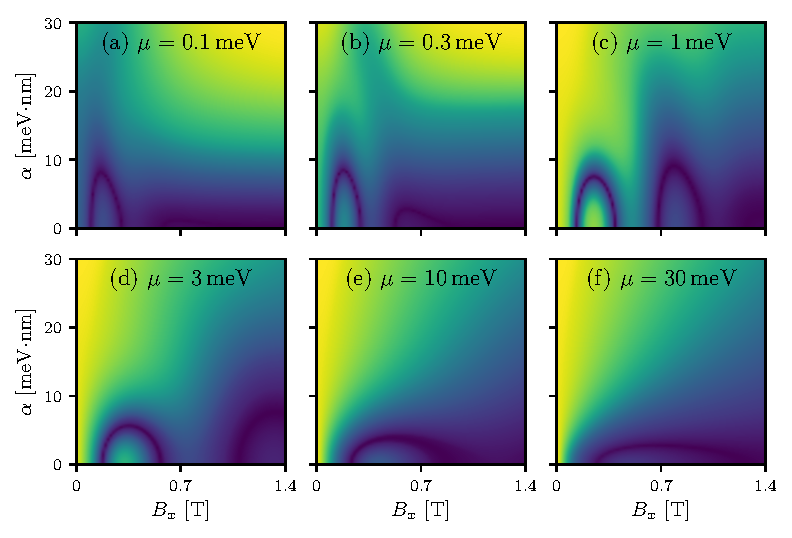
\includegraphics[width=0.75\columnwidth]{chapter_supercurrent/figures/sup_fig7}
\caption{Critical currents in a simple one-channel toy nanowire model\cite{Lutchyn2010,Oreg2010} as a function of spin-orbit coupling strength $\alpha$ and magnetic field along the wire $B_x$.
The different panels (a)-(f) are taken at different chemical potentials, $0.1,\; 0.3,\; 1,\; 3,\; 10,\; \SI{30}{meV}$ respectively.
The color scales are not normalized across the different panels, but are all separately scaled to optimally show all features in every plot.
We observe how the $0-\pi$ transitions at finite $B_x$ get mutually annihilated upon increasing $\alpha$.\label{fig:currents_1D_alpha_vs_B_x}}
\end{center}
\end{figure}

The previous discussion on spin related interference considered the Zeeman effect only.
However, the strong spin-orbit interaction in the nanowire fixes the spin direction to the propagation direction and thus counteracts the effect of the Zeeman splitting.
Following Ref.~\cite{Yokoyama2014}, the characteristic parameter for spin-orbit is $\theta_{SO} = \frac{\alpha k_\mathrm{F} L}{\hbar v_\mathrm{F}} = \frac{\alpha m^* L}{\hbar^2} = L/L_\mathrm{SO}$.
Here $L_\mathrm{SO}$ is the spin-orbit length, which is expected to be in the $50-\SI{250}{nm}$ range, much shorter than $L$.
For the Zeeman effect to cause a $0-\pi$ transition it needs to overcome the spin-orbit spin quantization.
This means that the spin-orbit term increases the field at which the first $0-\pi$ transition happens, and this increase is stronger as the chemical potential is further away from the band bottom.
This interplay between Zeeman and spin-orbit interaction is expected to be highly anisotropic\cite{Yokoyama2014} in the direction of $B$; the scenario described above assumes the external $B$ field and effective spin-orbit field to be perpendicular, as is expected for applying $B$ along the nanowire axis.
To substantiate our estimates we have used a nanowire toy model\cite{Lutchyn2010,Oreg2010} to obtain critical current as a function of gate voltage, magnetic field, and spin-orbit coupling in Fig.~\ref{fig:currents_1D_alpha_vs_B_x}.
The model indeed illustrates that the further the chemical potential is from the bottom of the band the higher is the value of the magnetic field at which the $0-\pi$ transition occurs.

In summary, the above estimates suggest that orbital interference is present regardless of the exact value of $\mu$, whereas spin related interference is highly restricted in $\mu$ range.
This favors an orbital interference interpretation of the experimental observations, since the supercurrent variations in the experiment are always present in a similar field range no matter the exact gate potential.

To illustrate this reasoning we produced Fig.~\ref{fig:currents_1D_alpha_vs_B_x}, which shows supercurrent fluctuations as a function of the distance to the bottom of the band in a single-band wire.
With increasing the distance to the bottom of the bands $0-\pi$ transitions happen at higher fields.
Upon ramping up spin-orbit strength the $0-\pi$ transitions disappear.

\subsection{Current phase relations and Josephson energies}\label{sec:cpr_jj_energies}
\begin{figure}
\begin{center}
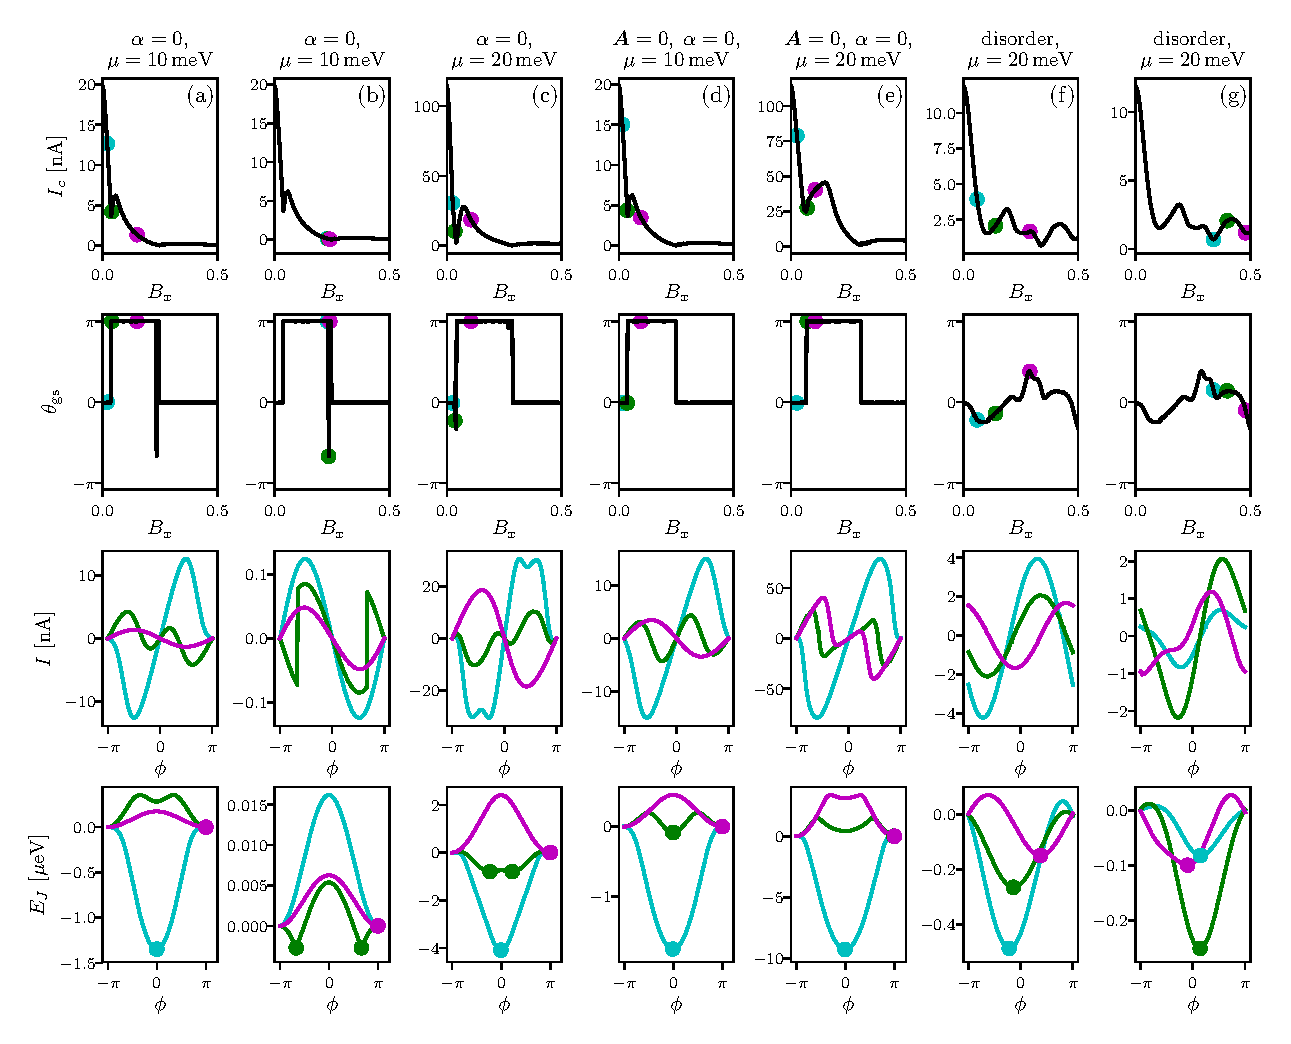
\includegraphics[width=1.0\columnwidth]{chapter_supercurrent/figures/sup_fig8.pdf}
\caption{(a)-(g) The critical current and ground state phase difference as function of magnetic field, and current phase relations (CPRs) and Josephson energies as functions of phase difference between the superconductors, for different parameters used in the model as labeled.
From top to bottom: $I_c(B_x)$ and $\theta_{\textrm{gs}}$ with the three points indicating the magnetic field values for which the CPR and $E_J(\phi)$ are plotted; CPRs for the three values of magnetic fields; Josephson energies as functions of the phase difference.
The dot in the bottom row $E_J$ indicates the energy minimum and the ground state phase difference.
Note that identical model parameters are used in columns (a),(b) and (f),(g) respectively, but different consecutive junctions states of interest are highlighted in the individual columns.
\label{fig:CPR}}
\end{center}
\end{figure}

To further support the claims of the previous section and to discuss the role of the ground state phase, we plot the evolution of the critical current and the ground state phase difference with magnetic field, and show the current-phase relations and Josephson energies characteristic for each junction state in Fig.~\ref{fig:CPR}.
$0-\pi$ transitions happen in the absence of spin-orbit interaction (Fig.~\ref{fig:CPR}(a)-(e)).
In the presence of spin-orbit and disorder, due to breaking of the spatial symmetry the ground state phase can obtain any single value $\varphi_0$ (a so-called $\varphi_0$-junction) near the crossover between $0$ and $\pi$ states of the junction ((Fig.~\ref{fig:CPR}(f)-(g)).
Note that without disorder, the spatial mirror symmetry with respect to the middle of the system forces all CPRs $I(\phi)$ to be odd functions and all $E_J(\phi)$ to be even functions of $\phi$.
When spatial mirror symmetry holds, the junction's Josephson energy can still have a double minimum at $\pm\varphi$ (a so called $\varphi$-junction), thus $E_J(\phi)$ taking a Mexican hat type shape (green curves in (Fig.~\ref{fig:CPR}(b)-(c)).
However, because of this restriction imposed by spatial mirror symmetry, $\varphi$-junctions are rare and most junctions are either 0 or $\pi$-junctions.
Contrarily, including disorder breaks this symmetry leading to commonly occurring $\varphi_0$-junctions.

\subsection{Effect of disorder}

\begin{figure}
\begin{center}
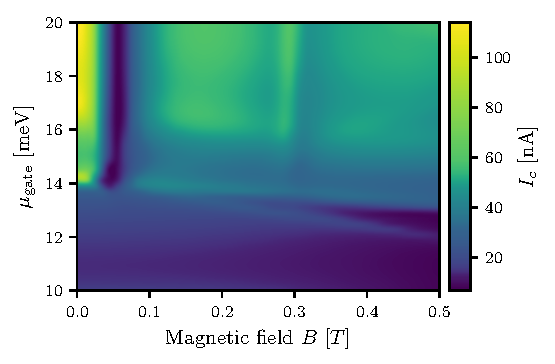
\includegraphics[width=0.7\columnwidth]{chapter_supercurrent/figures/sup_fig9.pdf}
\caption{Critical current as a function of the magnetic field and the gate voltage.
The simulation parameters are identical to the ones used in Fig.~\ref{fig:figure5}, but we set disorder to zero.\label{fig:gate_dependence}}
\end{center}
\end{figure}

Here we prove the essential effect of disorder on the supercurrent dependence on gate voltage.
We see the effect of disorder on $I_c(V_\textrm{gate})$ by comparing Fig.~\ref{fig:figure5}(b) and Fig.~\ref{fig:gate_dependence}, where we have switched off disorder.
In the clean case, where the main effect of the gate voltage on the supercurrent is via the gradual suppression of transmission through the nanowire, we observe that varying the gate voltage barely causes fluctuations of the supercurrent, even at finite magnetic field.
In the disordered case, changing the gate voltage effectively changes the realization of disorder in the region of the wire above the gate, thus causing supercurrent fluctuations.
With the increased disorder, the dwell time in the gated region of the nanowire is increased, so the gate voltage dependence increases with reduced mean free path.
We found that no disorder and disorder with mean free path greater than the system size cannot explain the observed dependence of the critical current on magnetic field and gate voltage.

\subsection{Rotating magnetic field}
\begin{figure}
\begin{center}
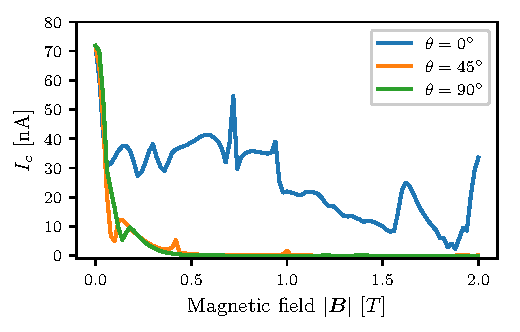
\includegraphics[width=0.7\columnwidth]{chapter_supercurrent/figures/sup_fig10}
\caption{
Supercurrent as a function of magnetic field for different directions of the applied field.
The angle is measured with respect to the wire axis and is rotated in the plane $\hat{x}$ parallel to the wire and $\hat{y}$ perpendicular to the wire and parallel to the substrate.
We use the same parameters as in Fig.~\ref{fig:figure5}.
Besides the field purely along $\hat{y}$ the fluctuations pattern is qualitatively similar in all the directions.}
\label{fig:rotation_of_field}
\end{center}
\end{figure}

Here we model the supercurrent fluctuations for different directions of the magnetic field, from parallel to the wire to perpendicular to it.
The results of the modeling are in Fig.~\ref{fig:rotation_of_field}.
We see that for all directions of the field, besides one parallel to the wire, the fluctuation pattern is basically the same.
This is in accordance with the experimental observations of Fig.~\ref{fig:angle_dependence}.

\references{dissertation}

% XXX: fix hard-coded fig nums
\chapter{Spin-orbit protection of induced superconductivity in Majorana nanowires}
\label{ch:spinorbit}

%% Start the actual chapter on a new page.
\newpage
\noindent
\section{Introduction}

Spin-orbit interaction (SOI) is a relativistic effect that results from electrons moving (orbit) in an electric field ($E$) experiencing a magnetic field ($B_{\mathrm{SO}}$) in their moving reference frame that couples to the electron's magnetic moment (spin).
SOI is an essential ingredient of various realizations of topological superconductors, which host Majorana zero modes, the building blocks of topological quantum computation \cite{Kitaev2001,Fu2008,Nayak2008}.
The prime platform for topological quantum computation is based on a semiconductor nanowire coupled to a superconductor, where the proximity effect opens a superconducting energy gap in the density of states of the nanowire \cite{Lutchyn2010,Oreg2010}.
In general, a magnetic field suppresses superconductivity by closing the superconducting gap due to Zeeman and orbital effects \cite{Nijholt2016}.
If the nanowire has strong SOI, suppression of the superconducting gap is counteracted and a sufficiently large Zeeman energy drives the system into a topological superconducting phase, with Majorana zero modes localized at the wire ends \cite{Lutchyn2010,Oreg2010}.
The main experimental effort in the last few years has focused on detecting these Majorana zero modes as a zero-bias peak in the tunneling conductance \cite{Mourik2012,Albrecht2016,Deng2016,Guel2018,Zhang2018,Lutchyn2018,Aguado2017}.
However, SOI, the mechanism providing the topological protection, has been challenging to detect directly in Majorana nanowires.

The electric field that gives rise to SOI in our system mainly results from structural inversion asymmetry of the confinement potential (Rashba SOI), which depends on the work function difference at the interface between the nanowire and the superconductor and on voltages applied to nearby electrostatic gates \cite{Vuik2016,Antipov2018,Woods2018,Mikkelsen2018}.
The Rashba SOI in nanowires has been investigated extensively by measuring spin-orbit related quantum effects: level repulsion of quantum dot levels \cite{Fasth2007,Nadj-Perge2012}, and of Andreev states \cite{Moor2018,Deng2016}, weak antilocalization in long \mbox{diffusive} wires \cite{Hansen2005,Weperen2015}, and a helical liquid signature in short quasiballistic wires \cite{Kammhuber2017}.
However, the SOI strength relevant to the topological protection is affected by the \mbox{presence} of the superconductor, necessitating direct observation of SOI in Majorana nanowires.
Here, we reveal SOI in an InSb nanowire coupled to a NbTiN superconductor through the dependence of the superconducting gap on the magnetic field, both strength and orientation.
We find that the geometry of the superconductor on the nanowire strongly modifies the direction of the spin-orbit field, which is further tunable by electrostatic gating, in line with the expected modifications of the electric field due to work function difference and electrostatic screening at the nanowire-superconductor interface.

Figure 1(a) shows the device image.
An InSb nanowire (blue) is covered by a NbTi/NbTiN superconducting contact (purple) and a Cr/Au normal metal contact (yellow).
The barrier gate underneath the uncovered wire (red) can deplete the nanowire, locally creating a tunnel barrier.
The tunneling differential conductance ($dI/dV$) resolves the induced superconducting gap, by sweeping the bias voltage ($V$) across the tunnel barrier [Fig. 1(b)].
The dashed arrow indicates the induced gap of 0.65 meV.
In this device, we have recently shown ballistic transport and Majorana signatures \cite{Guel2018}.

\begin{figure}
\begin{center}
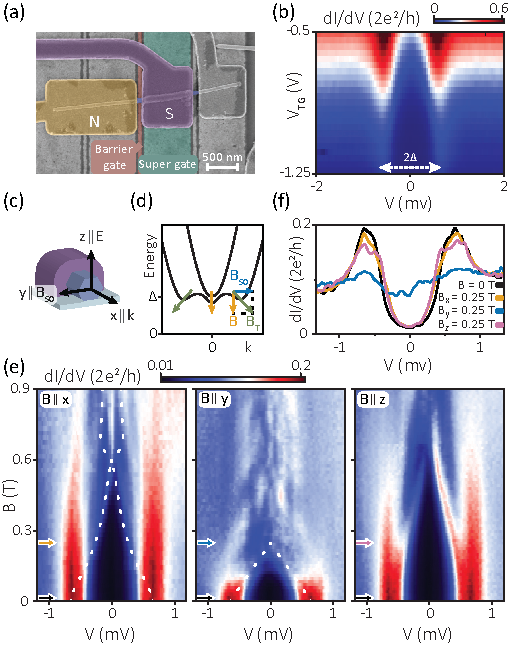
\includegraphics[width=0.7\columnwidth]{chapter_spinorbit/figures/Fig1.pdf}
\caption{\label{fig:fig1}
(a) False-color scanning electron micrograph of Majorana nanowire device $A$.
An InSb nanowire (blue) is contacted by a normal metal contact ($N$, yellow) and a NbTiN superconducting contact ($S$, purple).
The additional contact (gray) is kept floating.
The nanowire is isolated from the barrier gate (red) and the super gate (green) by $\sim$ 30 nm thick boron nitride.
(b) Differential conductance $dI/dV$ as a function of bias voltage $V$ and barrier gate voltage $V_{\mathrm{barrier}}$ at $B$ $=$ 0 T.
(c) Schematic of the nanowire device and definition of the axes.
(d) Band diagram of a Majorana nanowire at an externally applied magnetic field $B$ perpendicular to the spin-orbit field $B_{\mathrm{SO}}$.
The arrows indicate the total magnetic field $B_T$ $=$ $B$ + $B_{\mathrm{SO}}$ along which the spin eigenstates are directed.
At $k$ $=$ 0 the spin always aligns with $B$.
At increasing $k$, $B_{\mathrm{SO}}$ increases, tilting the spin more towards $B_{\mathrm{SO}}$.
(e) $dI/dV$ as a function of $V$ at $B$ along $x$, $y$, $z$ (left, middle, right) for super gate voltage $V_{\mathrm{SG}}$ $=$ 0 V.
The white dashed lines indicate a fit to the gap closing corresponding to $\alpha$ $=$ 0.15 $\pm$ 0.05 eV\AA.
(f) Horizontal line cuts of (e) at $B$ indicated by the colored arrows in (e).
}
\end{center}
\end{figure}

The magnetic field ($B$) dependence of the induced gap of device $A$, with $B$ along three different directions, is shown in Fig. 1(e).
The coordinate system is illustrated in Fig. 1(c).
The $x$ axis is along the nanowire, parallel to the electron momentum ($k$).
The $z$ axis is perpendicular to the substrate and coincides with the electric field ($E$) direction due to the spatial symmetry of the device and the bottom gate.
Since the Rashba spin-orbit field ($B_{\mathrm{SO}}$ $\propto$ $E$ $\times$ $k$) is perpendicular to both $k$ and $E$, it points along the $y$ axis.
When $B$ is aligned with $x$ or $z$ [left and right panels in Fig. 1(e)], both perpendicular to $B_{\mathrm{SO}}$, the gap closes \mbox{slowly} (at around 0.6 T), followed by the emergence of a zero-bias peak possibly characteristic of a Majorana zero mode when $B$ is along the nanowire, although we emphasize that a conjecture of Majorana zero modes is not essential for the purposes of this chapter.
On the contrary, when $B$ is aligned with the $y$ axis (middle panel), parallel to $B_{\mathrm{SO}}$, the gap closes much faster (at around 0.25 T).
Figure 1f shows the line cuts at $|B|$ $=$ 0.25 T along the three axes: for $B$ $\perp$ $B_{\mathrm{SO}}$, the gap is almost the same as when $B$ $=$ 0 T, while the gap is closed for $B$ $\parallel$ $B_{\mathrm{SO}}$.
This observation matches the predictions of the Majorana nanowire model, as illustrated in Fig. 1(d): when $B$ $\perp$ $B_{\mathrm{SO}}$, SOI counteracts the Zeeman-induced gap closing by rotating the spin eigenstate towards $B_{\mathrm{SO}}$, which reduces the component of the Zeeman field along the direction of the spin eigenstate.
In contrast, when $B$ $\parallel$ $B_{\mathrm{SO}}$, the spin eigenstate is always parallel to $B$, which prevents spin-orbit protection and results in a fast gap closing \cite{Osca2014,Rex2014}.
This pronounced anisotropy of the gap closing with respect to different $B$ directions is universally observed in over ten devices (four shown in this chapter) for all gate settings
\footnote{See Supplemental Material, which includes Refs.
 \cite{Car2014,Floehr2011,Suyatin2007,Guel2017,Liu2017,Danon2017,Hofstadter1976,Gropp1996,Du1999,Prada2012,Pientka2012,Stanescu2012}, for experimental details, theoretical details, and additional experimental data}, which is a direct consequence of SOI in Majorana nanowires.
\nocite{Car2014,Floehr2011,Suyatin2007,Guel2017,Liu2017,Danon2017,Hofstadter1976,Gropp1996,Du1999,Prada2012,Pientka2012,Stanescu2012}

Before we discuss the SOI in more detail, we rule out alternative mechanisms for the anisotropy which can originate in the bulk superconductor, or the InSb nanowire.
First, an anisotropic magnetic field-induced closing of the bulk superconducting gap is excluded for the fields we apply, which are far below the critical field of NbTiN ($>$9 T) \cite{VanWoerkom2015}.
We note that this is different from aluminium films \cite{Chang2015,Deng2016,Gazibegovic2017,Zhang2018}, where a small magnetic field ($<$0.3 T) perpendicular to the film completely suppresses superconductivity, making them unsuitable to reveal SOI from an anisotropic gap closing.
Next, we consider Meissner screening currents in NbTiN that can cause deviations in the magnetic field in the nanowire.
Our Ginzburg-Landau simulations show that the field corrections due to Meissner screening are negligible \cite{Note1}, since the dimensions of the NbTiN film ($<$1 $\mu$m) are comparable to the penetration depth ($\sim$290 nm).  % XXX: fix Note1
The simulations also show that vortex formation is most favorable along the $z$ axis \cite{Note1}, which implies that the observed anisotropic gap closing is not caused by gap suppression due to vortices near the nanowire \cite{Takei2013}, since we do not observe the fastest gap closing along $z$ [Fig. 1(f)].  % XXX: fix Note1
Finally, in the InSb nanowire, the Zeeman $g$ factor can become anisotropic due to quantum confinement \cite{Nadj-Perge2012,Pryor2006,Qu2016}.
However, our nanowire geometry leads to confinement in both the $y$ and $z$ directions, implying similar gap closing along $y$ and $z$, inconsistent with our observations [Fig. 1(e)].

Having excluded the above mechanisms, we are now left with three effects: spin splitting of the electron \mbox{states} in magnetic fields with the Land\'e $g$ factor (Zeeman eff\mbox{ect)}, the orbital effect of the magnetic field representing the Lorentz force acting on traveling electrons, and SOI.
To investigate the role of these effects, we use a theoretical three-dimensional Majorana nanowire model defined by the Hamiltonian \cite{Lutchyn2010,Oreg2010,Nijholt2016}:
\begin{equation*}
\begin{split}
H = &\left(\frac{\mathbf{p}^2}{2m^*}-\mu+V(y,z)\right) \tau_z + \frac{\alpha}{\hbar} \boldsymbol{\sigma} \cdot \mathbf{(\hat{E}\times p)} \tau_z\\
&+ \frac{1}{2}g\mu_B\mathbf{B\cdot}\boldsymbol{\sigma}+\Delta_0 \tau_x
\end{split}
\end{equation*}
Here, the first term represents the kinetic and potential energy, with $\mu$ the chemical potential measured from the middle of the helical gap and $V(y,z)$ $=$ $\frac{\Delta V_G}{R}[0,y,z]$ $\cdot$ $\mathbf{\hat{E}}$ is the electrostatic potential in the wire, whose magnitude is parametrized by $\Delta V_G$, with $\mathbf{\hat{E}}$ the direction of the electric field and $R$ the wire radius.
The orbital effect enters the Hamiltonian via the vector potential $\mathbf{A}$ in the canonical momentum: $\mathbf{p}$ $=$ $-i\hbar \nabla$ $+$ $e\mathbf{A}$.
Here, $e$ is the electron charge, $\hbar$ is Plank's constant, and $m^*$ $=$ 0.015 $m_e$ is the effective mass with $m_e$ the electron mass.
The second term represents Rashba SOI characterized by a SOI strength $\alpha$, which we set to 0.2 eV\AA\ to find qualitative agreement with the measurements.
The third term is the Zeeman term, with an isotropic $g$ factor set to 50 and $\mu_B$ is the Bohr magneton.
The last term accounts for the superconducting proximity effect, which we implement in the weak coupling approximation \cite{Nijholt2016}.
The Pauli matrices $\tau$ and $\sigma$ act in the particle-hole and spin space respectively.
We perform numerical simulations of this Hamiltonian on a 3D lattice in a realistic nanowire geometry using the \textsc{kwant} code \cite{Groth2014}.
We note that recent theory work shows that the anisotropy is unaffected by additional factors such as the wire length, temperature, and strong coupling to the superconductor \cite{Liu2019}.
Additional details are provided in the Supplemental Material \cite{Note1}.  % XXX: fix Note1

\begin{figure}
\begin{center}
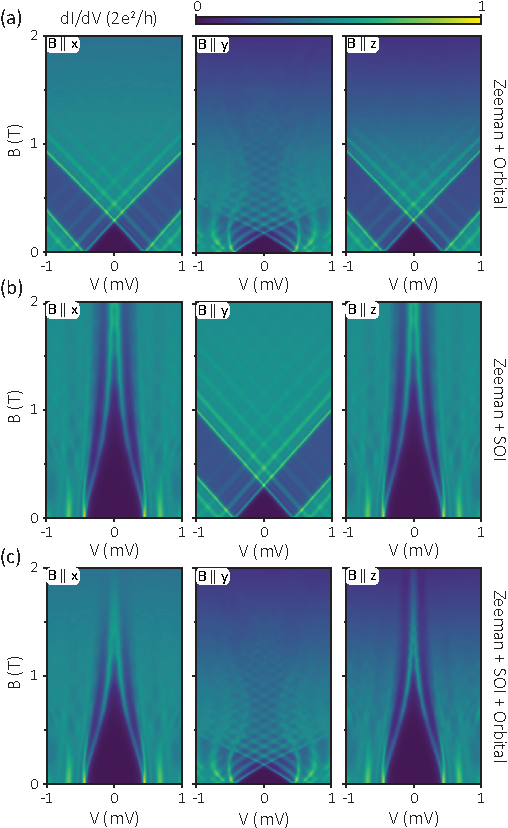
\includegraphics[width=0.7\columnwidth]{chapter_spinorbit/figures/Fig2.pdf}
\caption{\label{fig:fig2}
(a) Numerical simulations of $dI/dV$ as a function of $V$ and $B$, including the Zeeman and the orbital (Lorentz) effect of the magnetic field.
(b) Same as (a), but including Zeeman and SOI instead of the orbital effect, reproducing the anisotropy in Fig. 1(e).
(c) Same as (b), but including the Zeeman, SOI and orbital effect.
The parameters used in (a)-(c) are $\mu$ $=$ 5.6 meV and $\Delta V_G$ $=$ -8 meV.
}
\end{center}
\end{figure}

We identify which effects explain the observed anisotropic gap closing behavior by including them separately in our simulations.
Figure 2(a) shows the magnetic field dependence of the gap without SOI (setting $\alpha$ $=$ 0 in the Hamiltonian).
In contrast to Fig. 1(e) the gap closes around 0.3 T for all three directions, reflecting the dominant contribution of the Zeeman effect.
In Fig. 2(b), we turn on the SOI, and turn off the orbital effect by setting the magnetic vector potential $\mathbf{A}$ $=$ 0, which qualitatively reproduces the anisotropic behavior between the $y$ axis and the $x$ and $z$-axes.
We have explored other combinations of parameters and find that the experimental results of Fig. 1(e) can only be reproduced by including SOI.
We note that adding the orbital effect in Fig. 2(c) shifts the gap closing to a field almost twice as small for $B$ $\parallel$ $y$, which explains why we observe a gap closing for $B$ $\parallel$ $y$ at around 0.25 T, far below 0.45 T, the critical field expected when only the Zeeman effect with $g$ $=$ 50 suppresses the gap.
By fitting the curvature of the gap closing \cite{Heck2017,Pan2019} along $x$ [white dashed line in Fig. 1(e)] we estimate a range of the SOI strength $\alpha$ of 0.15 -- 0.35 eV\AA\ from devices $A$-$D$ (for fitting details and fits to additional devices, see Supplemental Material \cite{Note1}).  % XXX: fix Note1
This SOI strength is in \mbox{agreement} with the values extracted from level repulsion of Andreev states \cite{Stanescu2013,Moor2018} in an additional device $E$ \cite{Note1}.  % XXX: fix Note1
\mbox{Since} $\alpha$ depends on the electric field in the wire, we expect the observed variation in the SOI strength of devices to be caused by differences in the applied gate voltages and wire diameter.
Recently, the level repulsion of Andreev states in InSb nanowires covered with epitaxial aluminium has shown a SOI strength of approximately 0.1 eV\AA \cite{Moor2018}, slightly lower than we find for NbTiN covered nanowires, most likely due to strong coupling to the aluminium superconductor, leading to stronger renormalization of the InSb material parameters \cite{Stanescu2011,Cole2015,Antipov2018,Woods2018,Mikkelsen2018,Reeg2018}.

\begin{figure}
\begin{center}
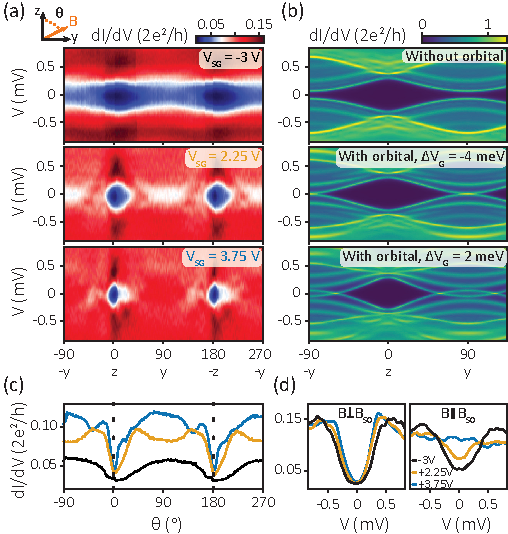
\includegraphics[width=0.7\columnwidth]{chapter_spinorbit/figures/Fig3.pdf}
\caption{\label{fig:fig3}
(a) Measured $dI/dV$ as a function of $V$ upon rotation of $B$ at 0.3 T over angles $\Theta$ between $z$ and $y$ in device $B$ (see Fig. S5 \cite{Note1} for the same behavior in device $A$).  % XXX: fix Note1
The voltage $V_{\mathrm{SG}}$ on the super gate (see insets) is varied in the three panels.
(b) Simulated $dI/dV$ as a function of $\Theta$ and $V$ at 0.25 T.
The top panel includes the Zeeman effect and SOI.
The middle and bottom panels additionally include the orbital effect at two values of the potential difference $\Delta V_G$ between the top and middle of the wire.
(c) Horizontal line cuts of (a) averaged over $|V|$ $<$ 0.2 V at $V_{\mathrm{SG}}$ $=$ -3,  2.25, and 3.75 V (black, orange, blue).
Dashed lines indicate the $z$ axis ($\Theta$ $=$ \ang{0}).
(d) Vertical line cuts of (a) at $\Theta$ $=$ \ang{0} (left) and $\Theta$ $=$ \ang{90} (right).
}
\end{center}
\end{figure}

To resolve the direction of the spin-orbit field, we fix the $B$ amplitude and continuously rotate the $B$ direction, parametrized by the angle $\Theta$ in the $zy$ plane [inset Fig. 3(a)].
Figure 3(a) shows the dependence of the gap on $\Theta$, where we adjust the electric field strength in the nanowire with a voltage $V_{\mathrm{SG}}$ on the super gate (SG) underneath the superconductor [green in Fig. 1(a)].
We define the angle at which the gap is hardest as $\Theta_{\mathrm{max}}$ and find $\Theta_{\mathrm{max}}$ $=$ 3 $\pm$ \ang{2} ($z$ axis) for all $V_{\mathrm{SG}}$ and in multiple devices (Fig. 3 and Fig. S5 \cite{Note1}) (error due to uncertainty in the extraction procedure).  % XXX: fix Note1
This is illustrated in Fig. 3(c), which shows horizontal line cuts for subgap bias.
The largest gap for a given $B$ amplitude is expected for $B$ $\perp$ $B_{\mathrm{SO}}$, indicating that $B_{\mathrm{SO}}$ $\parallel$ $y$, in agreement with the $E$-field direction dictated by the device geometry.

\begin{figure}
\begin{center}
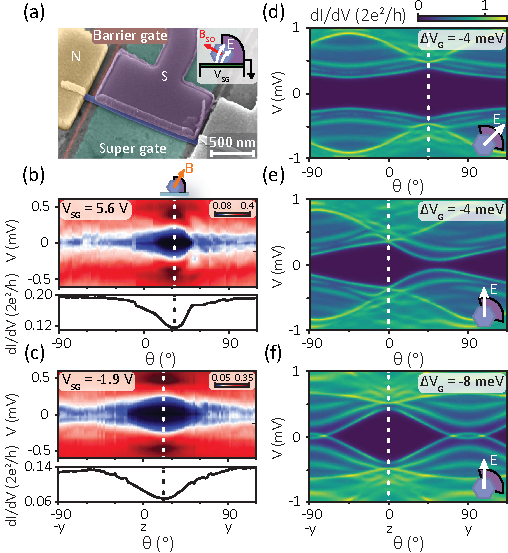
\includegraphics[width=0.7\columnwidth]{chapter_spinorbit/figures/Fig4.pdf}
\caption{\label{fig:fig4}
(a) Tilted view electron micrograph of Majorana nanowire device $E$, which is partially covered with NbTiN.
In this device, the electric field $E$ (and the associated spin-orbit field $B_{\mathrm{SO}}$) can rotate away from the $z$ axis ($y$ axis), as illustrated in the inset.
(b) Measured $dI/dV$ as a function of $V$ and angle $\Theta$ in the $zy$ plane at $|B|$ $=$ 75 mT and $V_{\mathrm{SG}}$ $=$ 5.6 V, with a horizontal line cut averaged over $|V|$ $<$ 0.25 mV in the lower panel.
The gap is maximum at $\Theta_{\mathrm{max}}$ $=$ \ang{32} as indicated by the dashed line.
(c) Same as (b), but at $V_{\mathrm{SG}}$ $=$ -1.9 V and $|B|$ $=$ 0.15 T.
$\Theta_{\mathrm{max}}$ is gate tuned to \ang{22}.
(d)-(f) Simulated $dI/dV$ at 0.25 T at various $\Delta V_G$ (see inset) with the superconductor rotated to the side by \ang{45} and including the Zeeman effect, SOI, and the orbital effect.
The illustrations in the insets indicate the direction of $E$, which is rotated by \ang{45} from $z$ in (d).
}
\end{center}
\end{figure}

Now, we check whether the orbital effect changes $\Theta_{\mathrm{max}}$.
The simulations in Fig. 3(b) show the effect of magnetic field rotation on the gap with $B_{\mathrm{SO}}$ $\parallel$ $y$, confirming that $\Theta_{\mathrm{max}}$ is, indeed, always given by the direction perpendicular to $B_{\mathrm{SO}}$, i.e.
$\Theta_{\mathrm{max}}$ $=$ \ang{0}.
Comparing the top panel (without the orbital effect) with the middle panel (with the orbital effect), we conclude that the orbital effect does not affect $\Theta_{\mathrm{max}}$.
This conclusion also holds when we vary the potential difference $\Delta V_G$ between the middle and outer of the wire (corresponding to $V_{\mathrm{SG}}$) in the middle panel and bottom panel.
We note that, at $\Delta V_G$ $=$ 2 meV (bottom panel) the wave function is moved towards the bottom of the nanowire, which increases the strength of the orbital effect by breaking the reflection symmetry about the $z$ axis, as evidenced by the longer angle range over which the gap is closed compared to $\Delta V_G$ $=$ -4 meV (middle panel).
Experimentally, we also observe this in Fig. 3(a), with line cuts in Fig. 3(c), where the gap is closed over a significantly longer angle range with increasing $V_{\mathrm{SG}}$.
We note that we use small values of $\Delta V_G$ in the simulations, because we expect a weak gate response due to effective electrostatic screening by the superconductor, which covers five of the six nanowire facets \cite{Zhang2017}.

Finally, we turn to a second type of device in which the superconducting film only partially covers the nanowire facets [Fig. 4(a)].
This partial superconductor coverage can modify the orientation of $B_{\mathrm{SO}}$ by changing the associated electric field direction \cite{Vuik2016}, as sketched in the inset of Fig. 4(a).
The electric field in the wire has two main origins.
The first one originates from the work function difference between the superconductor and nanowire, which leads to charge redistribution.
The resulting electric field is expected to rotate away from the $z$ axis due to the partial superconductor coverage which breaks the spatial symmetry.
In Fig. 4(b) we rotate $B$ in the $zy$ plane, perpendicular to the nanowire axis, and find that $\Theta_{\mathrm{max}}$ is, indeed, no longer at zero, but at 32 $\pm$ \ang{2}.
The second contribution to the electric field arises from the applied $V_{\mathrm{SG}}$ and the electrostatic screening due to the grounded superconductor.
Changing $V_{\mathrm{SG}}$ should, therefore, rotate the electric field for partial coverage.
Indeed, we find that $\Theta_{\mathrm{max}}$ shifts by \ang{10} by adjusting $V_{\mathrm{SG}}$ by 7.5 V [Fig. 4(c)].
Field rotation at intermediate $V_{\mathrm{SG}}$ and magnetic field sweeps confirming the change of $\Theta_{\mathrm{max}}$ are shown in the Supplemental Material \cite{Note1}.  % XXX: fix Note1
Our theory simulations confirm that $\Theta_{\mathrm{max}}$ is still given by the direction orthogonal to $B_{\mathrm{SO}}$ when the electric field is not necessarily along a \mbox{spatial} symmetry axis of the partially covered device [Fig. 4(d) and 4(e)].
While the orbital effect does not change $\Theta_{\mathrm{max}}$ [Fig. 4(e) and 4(f)], it can induce asymmetry in the energy spectrum around $\Theta_{\mathrm{max}}$ resulting from wave function asymmetry when the electric field is not along the mirror plane of the device [Fig. 4(b) and Fig. 4(e)].
The significance of the orbital effect in our devices underlines the importance of including it in realistic simulations of Majorana nanowires.

In conclusion, the observed gap closing anisotropy for different magnetic field orientations demonstrates SOI in our Majorana nanowires, a necessary condition to create Majorana zero modes.
Our experiments reveal that SOI is strongly affected by the work function difference at the nanowire-superconductor interface and the geometry of the superconductor, while electrostatic gating provides tunability of SOI.

\section{Appendix}

\subsection{Supplemental Experimental Details}
\subsubsection{Nanowire growth and device fabrication}
The \mbox{InSb} nanowires used here were grown using a Au-catalysed vapor-liquid-solid mechanism in a metal organic vapor phase epitaxy reactor, resulting in zinc blende nanowires grown \mbox{along} the [111] crystal orientation, which are free of stacking \mbox{faults} and dislocations \cite{Car2014}.
Local gates, covered by a h-BN dielectric flake, were fabricated on a silicon substrate.
The nanowires were individually placed over the gates using a micromanipulator \cite{Floehr2011}.
The contacts are fabricated by exposing the chip to a mild oxygen plasma cleaning after resist development, followed by immersion in a saturated ammonium polysulphide solution diluted by water to a 1:200 ratio for 30 minutes at \ang{60}C \cite{Suyatin2007}.
For the normal contacts, the wires are exposed to 30 seconds of in-situ helium ion milling, before evaporating 10 nm Cr and 110 nm Au.
The NbTiN contacts are fabricated by exposing the nanowire to 5 seconds or Ar plasma etching at 25 W, followed by sputtering of 5 nm NbTi and 85 nm NbTiN \cite{Guel2017,Zhang2017}.

\subsubsection{Measurement details}
The measurements were performed in a dilution refrigerator at an electron temperature of $\sim$ 50 mK  using a three-axis vector magnet and standard lockin techniques.

\subsection{Supplemental Theoretical Details}
\subsubsection{Details of the tight binding simulations}
The Hamiltonian defined in the main text is discretized on a lattice of a realistic nanowire geometry with a diameter of 70 nm and a length of 2 $\mu$m using a lattice spacing of 10 nm.
The nanowire is covered by a 35 nm thick superconducting shell covering 3/8 of the circumference of the wire, posititioned on top of the wire [Fig.~2, 3(b)] or rotated from the top to the side by \ang{45} [Fig.~4(b)].
Transport calculations are performed by connecting the nanowire to semi-infinite normal leads, separated by a tunnel barrier on one side.
The normal leads provide broadening of the peaks in the simulations \cite{Liu2017,Danon2017}.
The superconducting proximity effect is implemented using the weak coupling approximation \cite{Nijholt2016}, in which the pairing gap $\Delta_0$ $=$ 0 in the nanowire, which is tunnel coupled to a superconductor with $\Delta_0$ $>$ 0 providing an induced gap of 0.45 meV at $B$ $=$ 0 T.
The potential in the wire is given by $V(y,z)= \frac{\Delta V_G}{R} (z\cos(\Phi)+y\sin(\Phi))$, where $\Delta V_G$ is the potential difference between the middle and outer points of the wire, $R$ is the radius of the nanowire, and $\Phi$ parametrizes the direction of the electric field $\mathbf{\hat{E}}$, which is set to $\Phi$ = \ang{0} in all simulations, except for Fig.~4(d), where $\Phi$ = \ang{45}.
The vector potential $\mathbf{A} = \left[B_y(z-z_0)-B_z(y-y_0),0,B_x(y-y_0)\right]^T$ is chosen such that it does not depend on $x$ and the offsets $x_0$, $y_0$, $z_0$ are chosen such that the vector potential averages to zero inside the superconductor, implying a total supercurrent of zero in the superconductor.
This choice is supported by the negligible screening currents we observe in our Ginzburg-Landau simulations [Fig.~\ref{fig:GL}].
$\mathbf{A}$ is implemented in the tight-binding model by Peierls substitution in the hopping amplitudes \cite{Hofstadter1976}.

\subsubsection{Details of the Ginzburg-Landau simulations}
To calculate the stray fields in the nanowire due to Meissner screening and vortex entry in the superconducting contact (results shown in Fig.~\ref{fig:GL}), we have performed simulations on the Ginzburg-Landau model \cite{Gropp1996} in a realistic three-dimensional geometry using the dimensions of device A.
We used a penetration depth $\lambda$ = 290 nm and a Ginzburg-Landau parameter $\kappa = \lambda / \xi$ = 50, in line with the values expected for our NbTiN film, which has a room temperature resistivity of 95 $\mu \Omega$cm and a critical temperature of 15 K.
The Ginzburg-Landau functional is discretized both inside the superconducting contact as well as in its surrounding space \cite{Du1999} using a second-order finite difference scheme at a maximum internode distance of 0.01$\lambda$.
The resulting energy functional is minimized using the nonlinear conjugate gradient method and the code is implemented on a NVidia CUDA architecture with high parallelization.
We obtain the energy of states with vortices at finite magnetic fields by first introducing artificial perturbations near the sample boundary, followed by energy minimization to find the local minimum corresponding to a specific number of vortices.
The optimal number of vortices at a certain magnetic field is then determined by finding the state with the lowest energy globally.
We note that non-optimal amounts of vortices can be metastable due to significant Bean-Livingston barriers for vortex entry, so the actual number of vortices is hysteretic and depends on the dynamics of the magnetic field.

\begin{figure}
\begin{center}
\centering
\includegraphics[width=0.7\columnwidth]{chapter_spinorbit/figures/SFig2_GL.pdf}
\caption{\label{fig:GL}
Ginzburg-Landau simulations.
(a) The top panel shows the schematic of the geometry used for Ginzburg-Landau simulations: a superconducting film covering a hexagonal nanowire.
In a superconductor exposed to an external magnetic field $B$ we calculate the screening currents $I_{\mathrm{screening}}$, which induce stray magnetic fields $\Delta B$ in the nanowire.
In (b) we show $\Delta B$ in the $xy$-plane in the middle of the nanowire, as indicated by the white line in (a).
The bottom panel shows a top view of this $xy$-plane, where the arrows indicate the $x$ and $y$ components of $\Delta B$ in the nanowire for $B \parallel z$.
(b) The $x$, $y$ and $z$-components (black, yellow, blue) of $\Delta B$ relative to the external field $B$ as a function of the position $x$ along the nanowire axis, where $x = 0$ corresponds to the middle of the superconducting contact.
The lines show the mean stray field and the shaded regions are bounded by the minimum and maximum stray field found along the nanowire width at a particular $x$.
 The end of the superconducting film is indicated by the dashed line.
 $B$ is along $x$, $y$ and $z$ (left, middle and right panel).
Since the device dimensions are comparable to the penetration depth $\lambda = 290$ nm, the magnetic screening in the superconductor is incomplete, leading to small screening currents and stray fields of at most 4\% of $B$.
These modifications are much smaller and do not match the anisotropy we observe in the measurements, which excludes Meissner screening as the origin of the observed anisotropic gap closing.
We note that we have also evaluated $\Delta B$ at several different magnitudes of $B$ as well as in the presence of vortices and find relative stray fields of very comparable magnitude.
(c) Energetically most favorable number of vortices as a function of $B$ along $x$, $y$ and $z$ (black, yellow, blue).
Vortices form far more easily for $B \parallel z$.
An anisotropic gap closing due to vortices near the nanowire would therefore cause the fastest gap closing along $z$, contrary to the anisotropic gap closing we observe, where the gap closes fastest for $B \parallel  y$ [see e.g.
Fig.~1(e)].
Furthermore, for $B \parallel y$ vortices only start to appear at $B > 0.2$ T, while the gap is already strongly suppressed at 0.2 T [see e.g.
Fig.~1(e)], which excludes vortex formation as the origin of the gap closing for $B \parallel y$ and indicates that vortices do not have a strong effect on the size of the induced gap.
}
\end{center}
\end{figure}

\subsection{Extraction of SOI strength}
\subsubsection{Determination of SOI strength $\alpha$ from gap closing}
In a Majorana nanowire the SOI strength $\alpha$ determines the shape of the gap closing along $B$-directions perpendicular to the spin-orbit field $B_{\mathrm{SO}}$ \cite{Heck2017,Pan2019} [see Fig.~\ref{fig:SOIFit}(a)].
To find an analytical expression for the dependence of the gap closing on $\alpha$, we start from the conventional one-dimensional Majorana nanowire Hamiltonian \cite{Lutchyn2010,Oreg2010}, in which the gap size is given by the lowest energy eigenstate:
\begin{equation}
\Delta(B) = \min \bigg( \epsilon^2 + \epsilon_{\mathrm{SO}}^2 + \epsilon_{Z}^2 + \Delta(0)^2 \pm 2 \sqrt{\epsilon^2 ( \epsilon_{\mathrm{SO}}^2+\epsilon_{Z}^2 ) + \epsilon_{Z}^2\Delta(0)^2} \bigg)^\frac{1}{2}
\end{equation}
Here, $\epsilon=\hbar^2k^2/2m^*-\mu$ represents the kinetic energy, with $k$ the electron wave vector and $m^*=0.015 m_e$ the effective mass.
$\epsilon_{\mathrm{SO}}=\alpha k$ is the SOI term with $\alpha$ the SOI strength.
$\epsilon_Z = \frac{1}{2}g\mu_BB$ is the Zeeman energy, with $g$ the Land\'e $g$-factor and $\mu_B$ the Bohr magneton.
$\Delta(0)$ is the induced superconducting gap at $B = 0$ T, which we measure in the experiments (as indicated in Fig.~1(b)).

For $B \parallel B_{\mathrm{SO}}$ ($y$-axis) and neglecting the orbital effect the gap closes linearly with the Zeeman energy due to tilting of the bands \cite{Osca2014,Rex2014}:
\begin{equation}
\Delta(B) = \Delta(0) - \frac{1}{2}g\mu_BB
\end{equation}
The orbital effect significantly enhances the gap closing in our devices [cf.
Fig.~1,2], with a  strong dependence on the potential difference $\Delta V_G$ in the three-dimensional model.
Although the value of $\Delta V_G$ in our devices is unknown, we find that the orbital effect can be effectively taken into account in the one-dimensional model by adjusting the $g$-factor to match the gap closing along $B_{\mathrm{SO}}$, where SOI disappears and only the Zeeman and orbital effect contribute to the gap closing.
We emphasize that the $g$-factor extracted from the fits therefore does not correspond to the pure Zeeman $g$-factor used in our tight-binding calculations.
The validity of this approximation is demonstrated in Fig.~\ref{fig:SOIFit}(b), where the color map shows the gap closing resulting from our numerical calculations on the three-dimensional tight-binding model (taking the orbital effect into account and using $g = 50$) and the dashed white lines show the gap given by equation (S1) for $B\parallel x$ and by equation (S2) for $B\parallel y$ using $g=65$.

To extract $\alpha$ from our measurements, we fit the model given by equation (S1) and (S2) to the measured gap closing both along the wire and along $B_{\mathrm{SO}}$ simultaneously.
We prevent overfitting by independently constraining the free parameters.
First, $g$ is determined by the gap closing along $B_{\mathrm{SO}}$, which only depends on the Zeeman effect.
Then, $\mu$ follows from the critical field $B_C$ along $x$, where $\frac{1}{2}g\mu_BB_C = \sqrt{\Delta(0)^2+\mu^2}$ \cite{Lutchyn2010,Oreg2010} (note that $B_C$ does not depend on $\alpha$).
The SOI strength $\alpha$ is now the only free parameter left to fit the curvature of the gap closing along $x$.
This procedure is applied to four devices [see Fig. 1(f), Fig.~\ref{fig:BsweepsReproduced}(b),(c), and Fig.~\ref{fig:BsweepsHalf}], resulting in a SOI strength of 0.15 -- 0.35 eV\AA, corresponding to a spin-orbit energy $E_{\mathrm{SO}}=m^*\alpha^2/2\hbar^2$ of 20 -- 120 $\mu$eV.
The remaining parameters used for the fit of device A shown in Fig.~1(e) are $g$ = 90, $\mu$ = 1.4 meV.
The values of $g$ and $\mu$ found for the remaining devices are given in Fig.~\ref{fig:BsweepsReproduced}.
Table I shows the range of values of the fitting parameters for which good fits can be obtained.
Since $\alpha$ depends on the electric field in the wire, we expect the observed variation in the SOI strength of devices to be caused by differences in the applied gate voltages and wire diameter.

\begin{table}[h]
\label{tab:AlphaFit}
\caption{Results of gap closing fitting procedure}
\begin{tabular}{l|cccc}
& Device A & Device B & Device C & Device D \\
\hline
$g$ & 90 $\pm$ 10 & 60 $\pm$ 20 & 85 $\pm$ 5 & 160 $\pm$ 20\\
$\mu$ (meV) & 1.5 $\pm$ 0.4 & 1.8 $\pm$ 0.8 & 2.75 $\pm$ 0.25 & 2.8 $\pm$ 0.6\\
$\alpha$ (eV\AA) & 0.15 $\pm$ 0.05 & 0.3 $\pm$ 0.1 & 0.35 $\pm$ 0.05 & 0.35 $\pm$ 0.05\\
\end{tabular}
\end{table}

\begin{figure}
\begin{center}
\centering
\includegraphics[width=0.7\columnwidth]{chapter_spinorbit/figures/SFig7_AlphaFitting.pdf}
\caption{\label{fig:SOIFit}
Extracting SOI strength from gap closing curvature.
(a) Lowest energy state $E_{\mathrm{min}}$ determining the gap in the one-dimensional model given by equation S1 as a function of magnetic field, $B$, in units of the critical field $B_c=\sqrt{\Delta^2+\mu^2}$ for various spin-orbit strengths $\alpha$.
The curvature of the gap closing is strongly affected by $\alpha$.
Stronger SOI counteracts the Zeeman effect up to larger $B/B_c$, leading initially to a slow gap closing, followed by a sharp gap closing when approaching the critical field, where the lowest energy state is at $k \approx 0$ for which $B_{\mathrm{SO}}(k)$ vanishes.
The remaining parameters are: $\Delta(0)$ = 1 meV, $\mu$ = 2 meV.
(b) Comparison of the numerical simulations on the 3D tight binding model, including the orbital effect (color map), with the 1D model given by equations (S1) and (S2) which does not account for the orbital effect (dashed lines).
By adjusting the $g$-factor used in the Majorana nanowire model from $g$ = 50 to 65 to match the gap closing for $B \parallel B_{\mathrm{SO}}$, keeping all other parameters the same in both models, we find good agreement for the gap closing for $B \parallel x$.
We use this same approach to take the orbital effect into account in an effective manner in fits of the experimentally observed gap closing.
The remaining parameters used in the simulations shown here are $\Delta(0)$ = 0.45 meV, $\mu$ = 0.95 meV, $\alpha$ = 0.2 eV\AA, $\Delta V_G$ = -10 meV.
}
\end{center}
\end{figure}

\subsubsection{Estimation of SOI strength based on level repulsion}
SOI induces coupling between states of different momentum and spin in finite length Majorana nanowires, which leads to level repulsion when energy levels are nearly degenerate \cite{Stanescu2013}.
Recently this level repulsion between longitudinal states within the same subband was used to estimate a SOI strength in epitaxial Al-InSb nanowires \cite{Moor2018}.
Here, we follow the same procedure to estimate the SOI strength in a seperate device with a NbTiN superconductor that exhibits such level repulsion.
We consider a low energy model of two levels dispersing in the magnetic field due to the Zeeman effect, coupled to each other by SOI with the matrix element $\delta_{\mathrm{SO}}$:

\begin{equation}
H = \begin{bmatrix}
E_0 + \frac{1}{2}g_0 \mu_B B & \delta_{\mathrm{SO}} \\
\delta_{\mathrm{SO}} & E_1 - \frac{1}{2}g_1 \mu_B B
\end{bmatrix}
\end{equation}

We fit the eigenenergies of $H$ to our experimental data [Fig.~\ref{fig:SOIlevelrep}a] to extract $\delta_{\mathrm{SO}}$.
The precise value of the coupling parameter $\delta_{\mathrm{SO}}$ depends not only on $\alpha$, but also on the details of the confinement and on the coupling strength to the superconductor \cite{Moor2018}.
A rough estimate, with reasonable agreement to numerical simulations, was proposed to be: $2\delta_{\mathrm{SO}}$ = $\alpha \pi/ L$, where $L$ is the length of the wire.
The extracted $\delta_{\mathrm{SO}}$ is shown in Fig.~\ref{fig:SOIlevelrep}(b) for various values of the super gate voltage $V_{\mathrm{SG}}$.
As $V_{\mathrm{SG}}$ becomes more negative, we see an increase in $\delta_{\mathrm{SO}}$, consistent with an increasing electric field in the nanowire.
We can estimate $\alpha \sim$ 0.4 -- 0.55 eV\AA.
Considering the uncertainty in the relation between $\alpha$ and $\delta_{\mathrm{SO}}$ and variation in the electrostatic environment of different devices, this magnitude is in line with our estimation based on the gap closing curvature.

\begin{figure}
\begin{center}
\includegraphics[width=0.7\columnwidth]{chapter_spinorbit/figures/SFig3_Anticrossing.pdf}
\caption{\label{fig:SOIlevelrep}
Extracting the SOI strength from level repulsion.
(a) $dI/dV$ as a function of $V$ and $B$ at $V_{\mathrm{SG}}$ = -3.3 V, measured in device E.
Two Andreev states come down from the gap edge and exhibit an avoided crossing around $B = 0.5$ T.
The dashed lines indicate fits to the solution of equation (S3).
The extracted coupling $\delta_{\mathrm{SO}}$ between the Andreev levels is indicated by the arrow.
(b) $2\delta_{\mathrm{SO}}$ as a function of $V_{\mathrm{SG}}$.
The right axis shows the estimation of the SOI strength using $\alpha = 2\delta_{\mathrm{SO}}L/\pi$ for the 1.2 $\mu$m long superconducting region.
The errorbars show the standard deviation in $\delta_{\mathrm{SO}}$ obtained from the fits.
}
\end{center}
\end{figure}

\clearpage
\subsection{Supplemental Experimental Data}

\begin{figure}
\begin{center}
\centering
\includegraphics[width=0.7\columnwidth]{chapter_spinorbit/figures/SFig1_Bsweeps_reproduced.pdf}
\caption{\label{fig:BsweepsReproduced}
Anisotropic gap closing in additional devices.
(a) False colored scanning electron micrographs of additional devices B (used in Fig.~3) and C, showing anisotropy similar to the device in Fig.~1(e).
(b,c) Differential conductance, $dI/dV$, as a function of the magnetic field, $B$, along the $x$, $y$, and $z$-axes (from left to right).
The gap closes at much lower fields along the $y$-axis than the $x$ and $z$-axes in all devices fully covered with the superconductor.
The white dashed lines indicate fits to the gap closing from which we extract a spin-orbit strength $\alpha$ of 0.3 $\pm$ 0.1 eV\AA\ [for (b)] and 0.35 $\pm$ 0.05 eV\AA\ [for (c)], with $g$ = 60, 85 and $\mu$ = 1.8, 2.7 meV as the remaining fit parameters for (b), (c) respectively.
We note that we do not observe clear reopening of the gap in all devices, which theoretical studies have attributed to the negligible contribution to the tunneling conductance of the states associated with the gap reopening due to their spatial wave function extension into the middle of the wire leading to minimal weight near the tunnel barrier \cite{Prada2012,Pientka2012,Stanescu2012,Liu2019}.
The super gate was set to $V_{\mathrm{SG}}$ = -1.5 V, -2.6 V in (b), (c) respectively.
}
\end{center}
\end{figure}

\begin{figure}
\begin{center}
\centering
\includegraphics[width=0.7\columnwidth]{chapter_spinorbit/figures/SFig4_YZrot_Full1_reproduced.pdf}
\caption{\label{fig:YZrotRep}
Gap dependence on magnetic field orientation in \textit{zy}-plane in device A.
(a) Differential conductance, $dI/dV$, as a function of bias voltage, $V$, upon rotation of the magnetic field at 0.25 T over angles $\Theta$ between $z$ and $y$ with different voltages on the super gate $V_{\mathrm{SG}}$ in the three panels.
This is the same device as presented in Fig.
1 (b) Horizontal line cuts of (a) averaged over a bias range $|V| < 0.2$ mV, showing that the hardest gap is at $\Theta = 0$, and increased $V_{\mathrm{SG}}$ suppresses the gap when $B$ is along $y$, the same behaviors observed in device B [Fig.~3].
}
\end{center}
\end{figure}

\begin{figure}
\begin{center}
\centering
\includegraphics[width=0.7\columnwidth]{chapter_spinorbit/figures/SFig5_SGdep_half_updated.pdf}
\caption{\label{fig:SGdep}
Dependence of spin-orbit direction on super gate voltage in device D, which is partially covered by NbTiN.
(a) Differential conductance, $dI/dV$, as a function of bias voltage, $V$, and angle $\Theta$ between $z$ and $y$ at various values of $V_{\mathrm{SG}}$ as indicated in the insets.
The data is measured at slightly different field magnitudes between 0.1 and 0.2 T for the different $V_{\mathrm{SG}}$ to optimize the anisotropy between $y$ and $z$.
The discontinuities in $dI/dV$ that are visible for some of the scans are likely caused by charge fluctuations in the dielectric environment.
(b) The ratio between the sub gap conductance (averaged over $|V| < 0.2$ V) and the above gap conductance (averaged over $|V| > 0.4$ V) with $V_{\mathrm{SG}}$ increasing from bottom to top and offset for clarity.
The minima of the curves signify the angle at which the gap is hardest, $\Theta_{\mathrm{max}}$, which shifts to higher angles at increasing $V_{\mathrm{SG}}$.
A lowpass filter is applied along the $\Theta$ direction to suppress the effect of the charge instabilities (this procedure does not affect the minima for the measurements without charge instabilities, such as in Fig.~4).
(c) $\Theta_{\mathrm{max}}$ as determined from the first (black) and second (yellow) minimum of the curves in (b) as a function of $V_{\mathrm{SG}}$.
The second minima (yellow) signify $\Theta_{\mathrm{max}}$ at negative $B$ and are subtracted by \ang{180} accordingly.
}
\end{center}
\end{figure}

\begin{figure}
\begin{center}
\centering
\includegraphics[width=0.7\columnwidth]{chapter_spinorbit/figures/SFig6_Bsweeps_half.pdf}
\caption{\label{fig:BsweepsHalf}
Gap dependence on magnetic field orientation in device E, which is partially covered by NbTiN.
(a) Differential conductance, $dI/dV$, as a function of the angle $\Theta$ between the $z$ and $y$-axes at $V_{\mathrm{SG}}$ = 0.525 V and $B$ = 0.1 T, with a horizontal line cut averaged over a bias range $|V| < 0.3$ mV in the lower panel.
(b) $dI/dV$ as a function of the magnetic field $B$ along the nanowire axis, with the white dashed lines showing the fit to the gap closing, resulting in a spin-orbit strength $\alpha$ of 0.35 $\pm$ 0.05 eV\AA\ (the other fit parameters are $g$ = 160, see $B \parallel B_{\mathrm{SO}}$ in (c), and $\mu$ = 2.8 meV).
(c) $dI/dV$ as a function of $B$ along $y$, $B_{\mathrm{SO}}$, $z$ and perpendicular to $B_{\mathrm{SO}}$ from left to right, with the colors in the headers corresponding to the colored arrows in (a).
The illustrations in the insets indicate the direction of the magnetic field.
Note that due to the changed orientation of $B_{\mathrm{SO}}$, $B$-sweeps along directions rotated by $\sim$\ang{25} from the $y$-axis (second panel, $B \parallel B_{\mathrm{SO}}$) and the $z$-axis (right panel, $B \perp B_{\mathrm{SO}})$  now exhibit strong anisotropy, instead of the $y$ and $z$-axes which show strong anisotropy in devices symmetrically covered by NbTiN.
}
\end{center}
\end{figure}

\references{dissertation}

\chapter{Enhanced proximity effect in zigzag-shaped Majorana Josephson junctions}
\label{ch:zigzag}

%% Start the actual chapter on a new page.
\newpage
\noindent 
\section{Introduction}

\cite{Beenakker1992} % XXX: it needs a citation

\references{dissertation}

\chapter{Extracting the spin-orbit coupling strength from weak anti-localization measurements using realistic device simulations}
\label{ch:weakantilocalization}

%% Start the actual chapter on a new page.
\newpage
\noindent 
\section{Introduction}



\references{dissertation}
\chapter{Robustness of Majorana bound states in the short-junction limit}
\label{ch:shortjunction}

\blfootnote{This chapter has been previously published as
Doru Sticlet, Bas Nijholt, and Anton R. Akhmerov, \textit{Robustness of Majorana bound states in the short-junction limit}, \href{https://doi.org/10.1103/PhysRevB.95.115421}{Phys. Rev. B \textbf{95}, 115421, (2017)}
}

%% Start the actual chapter on a new page.
\newpage
\noindent

\section{Introduction}
\co{Long vs short Josephson junction}
The theory of normal conductor-superconductor (NS) hybrid systems distinguishes two limiting cases: long and short junctions.
In long junctions, the dwell time $\tau_\textrm{dw}$ of a quasiparticle inside the normal region is much larger than the time $\hbar/\Delta$ it spends inside the superconductor (with $\Delta$ the superconducting gap).
In this limit the induced gap inside the semiconductor is equal to $\hbar/\tau_{\textrm{dw}}$, and therefore it varies for different bound states.
In the short-junction or strong-coupling limit, the quasiparticles spend most of their time inside the superconductor, while the normal region effectively acts as a delta function scatterer.
Then in the presence of time-reversal symmetry, the induced gap is close to $\Delta$ for every single Andreev bound state.
In the short-junction limit Andreev bound states have the most weight in the superconductor, and therefore the conventional approach of integrating out the superconductor and obtaining an effective Hamiltonian of the normal system becomes inefficient due to the strong energy dependence of the effective Hamiltonian.

\co{MBS in short-junction limit}
Systematically studying the short-junction limit is relevant for the creation of Majorana bound states (MBS)~\cite{Qi2011, Leijnse2012, Alicea2012, Beenakker2013, Elliott2015} in semiconductor nanowires\cite{Lutchyn2010, Oreg2010} partially coated with epitaxially grown aluminum that have high interface quality.
These systems were observed to have a well-developed hard induced gap comparable to the gap in the bare Al~\cite{Chang2015}, and subsequently showed zero bias peaks~\cite{Deng2016} and suppressed splitting of low energy states characteristic to MBS~\cite{Albrecht2016}.
The theoretical description of the response of strongly coupled zero-dimensional NS junctions to magnetic field was analyzed in Ref.~\cite{Cole2015}, where the authors report a strong suppression of the effective $g$ factor, potentially leading to the impossibility of inducing a topological phase at magnetic fields below the Clogston limit~\cite{Clogston1962}.

\co{Use scattering formalism}
Here we extend the analysis of Ref.~\cite{Cole2015} using the scattering formalism that allows us to capture the nonlinear features of the spectrum, and by considering higher-dimensional systems with translational invariance.
The scattering formalism has been routinely applied to short junctions in mesoscopic physics [for review see ~\cite{Beenakker2005}].
Relevant works to the present study are on two-dimensional electronic gases with spin-orbit interactions~\cite{Bezuglyi2002, Dimitrova2006}.
However, in Majorana literature the use of the scattering formalism has been limited~\cite{Cheng2012}.
The equivalent of the scattering formalism using the effective Hamiltonian approach amounts to introducing an effective self-energy $\Sigma(E)$ which has a proper dependence on energy $E$~\cite{Liu2012, Stanescu2013, Peng2015} and then neglecting the energy term in the nonlinear eigenvalue problem $[H-\Sigma(E)]\psi = E\psi$, as done in, e.~g.,~Ref.~\cite{Poeyhoenen2016}.

\co{We find that it is not so bad}
Our overall findings are favorable for the creation of MBS in Al-based NS systems.
Specifically, we find that:
\begin{itemize}
\item The critical magnetic field $B_*$ required to induce a topological phase is independent of the superconducting gap.
 This is valid also beyond the short-junction limit, as long as penetration of magnetic field into the superconductor is negligible.
\item Since $B_*$ is inversely proportional to the wire cross section, the device design can be used to adjust $B_*$ within a broad range.
\item The localization length $\xi_M$ of the MBS does not depend on the superconducting gap, and in optimal conditions it is proportional to the spin-orbit length $l_\textrm{SO}$.
\item Finally, if the interface between the semiconductor and the superconductor has high transparency $T$, then $B_*$ becomes only a slowly varying function of the chemical potential $\mu$, as opposed to its usual oscillatory behavior on the scale of the mode spacing in the nanowire~\cite{Wimmer2010, Lutchyn2011}.
\end{itemize}
Our analytical calculations fully coincide with the results obtained using a numerical scattering approach to short junctions and exact diagonalization of a discretized tight-binding Hamiltonian.
While these conclusions are favorable for the prospect of using weak superconductors for MBS creation, we note that the effects of disorder in the superconductor are not systematically treated here.
Disorder has been recently predicted to have a strong detrimental effect on the creation of MBS in systems that are in the short-junction limit~\cite{Cole2016}.

\co{Organization of the chapter}
This chapter is organized as follows.
Section~\ref{sec:formalism} contains a pedagogical review of scattering formalism for the calculation of Andreev spectrum.
The following Sec.~\ref{sec:jjintro} presents scaling arguments supporting our conclusions.
In Sec.~\ref{sec:1stmodel} we compute the dispersion relation of a planar NS junction and discuss the typical device parameters.
Section~\ref{sec:topphases} investigates the Majorana phase diagram and the behavior of the MBS decay length.
In Sec.~\ref{sec:finite} we compare the predictions of Sec.~\ref{sec:topphases} with numerical diagonalization of finite junctions.
Section~\ref{sec:orb} estimates the orbital effect of the magnetic field by computing the Andreev spectrum in a cylindrical geometry in a thin shell limit.
In Sec.~\ref{sec:3d} we confirm our findings using a numerically computed Majorana phase diagram of a three-dimensional model.
Lastly, section~\ref{sec:conc} sums up our conclusions.

\section{Scattering matrix formalism and the short-junction limit}
\label{sec:formalism}
This section reviews the scattering approach to calculating the Andreev bound state spectrum and may be skipped by expert readers.
We start by considering a general NS junction with $n$ superconducting terminals.~\cite{Heck2014}
We use the case $n=1$ in Secs.~\ref{sec:1stmodel},~\ref{sec:topphases},~\ref{sec:3d} and $n=2$ in Sec.~\ref{sec:orb}.

\co{Andreev bound states condition.}
The levels with $|E|<\Delta$ are Andreev bound states, i.e., coherent superpositions of electron and hole excitations which occur due to Andreev reflections~\cite{Andreev1964} at the interface between the normal region and the superconducting terminals.
The wave function quantization condition on the wave function requires that the total sequence of scattering events results in a phase shift of $2\pi n$.
For the vector of modes $\psi$ incoming from the superconductor to the normal region this condition reads:
\begin{equation}\label{bound}
S_A S_N\psi=\psi.
\end{equation}
Here $S_N$ is the scattering matrix of the normal region, and $S_A$ the scattering matrix of Andreev reflection processes in the superconducting terminals.
The mode vector has electron and hole components $\psi=(\psi_e, \psi_h)$.

\co{Different bases}
The Andreev reflection matrix assumes a universal form when the superconductor has $s$-wave pairing without any sources of time-reversal symmetry breaking and additionally when the Andreev approximation holds (when the Fermi energy in the superconductor is much larger than $\Delta$).
In the literature, the Andreev spectrum is often calculated in systems where the superconductor Hamiltonian has full spin-rotation invariance (an appropriate approximation for aluminum), making the spin basis a natural choice of basis of $\psi$.
Yet the universal structure of the Andreev reflection matrix does not change in the presence of spin-orbit coupling in the superconductor.
However, in that case it is impossible to choose a spin basis due to lack of spin conservation and it is more appropriate to use a basis where the outgoing modes are time reversed of the incoming modes~\cite{Bardarson2008}.
Throughout this chapter we work in the latter basis but explain the relation to the more commonly used spin basis for reference at the end of this section.
Importantly, we neglect the time-reversal symmetry breaking perturbations in the superconductor, restricting ourselves to magnetic fields much lower than critical.

\co{Normal state scattering matrix.}
The scattering matrix of the normal region is block diagonal in the Nambu space:
\begin{equation}
S_N(E,\mathbf k)=\pmat{S_e(E,\mathbf k) & 0 \\
0 & S_h(E,\mathbf k)},
\end{equation}
where $S_e$ and $S_h$ are the scattering matrices of electrons and holes.
We consider NS junctions with a translational symmetry, and therefore the scattering matrices may depend on the wave vector $\mathbf k$ along the translationally invariant directions.
We choose the hole modes $\psi_e$ as particle-hole partners of the electron modes $\psi_e$.
In this basis the particle-hole symmetry of the scattering matrix reads:
\begin{equation}
\tau_x S^*_N(E,\mathbf k)\tau_x=S_N(-E,-\mathbf k),\label{eq:phs}
\end{equation}
Using the block-diagonal structure of $S_N$ it follows that the normal scattering matrix of holes is the conjugate of the scattering matrix for electrons, at opposite energy and momentum~\cite{Beenakker2015}:
\begin{equation}\label{phs}
S_h(E,\mathbf k)=S_e^*(-E,-\mathbf k).
\end{equation}

\co{Andreev reflection matrix}
In the same basis, the Andreev reflection matrix reads:
\begin{equation}\label{areflmat}
S_A=\alpha(E)R,\quad R=\pmat{0 & r\\ -r^* & 0},
\quad r=\oplus_j e^{i\phi_j},
\end{equation}
where the index $j$ runs over the terminals, $\phi_j$ is the superconducting phase in lead $j$, and $\alpha(E)=\exp(-i\arccos(E/\Delta))$.~\cite{Beenakker1991}

Following Ref.~\cite{Beenakker1991}, eliminating $\psi$ from Eq.~\eqref{bound}, and using an expression for a block matrix determinant one immediately arrives to a determinantal equation for the bound state energies:
\begin{equation}\label{det}
\det[
1+\alpha^2(E)r^*S_e(E,\mathbf k)rS^*_e(-E,-\mathbf k)
]=0.
\end{equation}
The short-junction limit allows us to further simplify the calculation of the Andreev bound state energies when Thouless energy $E_\textrm{Th} \equiv \hbar/\tau_\textrm{dw} \gg \Delta$.
Thouless energy is the typical energy scale for the matrix elements to change appreciably, therefore in the short-junction limit $S_N(E, \mathbf k) \approx S_N(0, \mathbf k)$ for any $E\lesssim \Delta$.
After replacing $S_e(E)$ with $S_e(0)$, the only energy-dependent term remaining in Eq.~\eqref{bound} is the coefficient $\alpha(E)$.
Since the scattering matrices are invertible, Eq.~\eqref{bound} reads:
\begin{equation}
RS_N\psi
=\alpha^{-1}(E)\psi,\textrm{ or }
S_N^{-1}R^{-1}\psi
=\alpha(E)\psi.
\end{equation}
Adding the two equations yields the following energy eigenproblem:
\begin{equation}
\frac{1}{2}[RS_N+S_N^{-1}R^{-1}]\psi
=\frac{E}{\Delta}\psi.
\end{equation}
Further squaring this equation and using the unitarity of the scattering matrices $S_A$ and $S_N$ we arrive to the eigenproblem expression for the Andreev spectrum:
\begin{equation}\label{nsspec}
\left\{
\frac{1}{2}-\frac{1}{4}
\big[
S_e^\dag(\mathbf k)rS_e^T(-\mathbf k)r^*+\mathrm{H.c.}
\big]
\right\}\psi_e=\frac{E^2}{\Delta^2}\psi_e,
\end{equation}
where the energy argument is suppressed, since $S_e$ is evaluated at $E=0$.
If there is only a single superconducting terminal, the Andreev reflection matrix $r$ reduces to a phase factor, which fully drops out from Eq.~\eqref{nsspec}, as required by gauge invariance.

If the spin is conserved, the above derivation is nearly identical in the spin basis.
The scattering matrices in the spin basis $\tilde S_e$ and $\tilde r$ are related to the basis of time-reversed modes by a transformation
\begin{equation}
\tilde S_{e}=-i\sigma_yS_{e},\quad\tilde r=-i\sigma_y\oplus_j e^{i\phi_j},
\end{equation}
with the Pauli matrices $\bm\sigma$ spin operators and $\sigma_0$ an identity matrix.
The symmetry condition~\eqref{phs}, equation~\eqref{det} for the Andreev spectrum, and eigenproblem for the spectrum in short-junction approximation~\eqref{nsspec} are identical in both bases upon replacing $S_e$ and $r$ with $\tilde S_e$ and $\tilde r$.


\section{Scaling arguments for the MBS properties in the short-junction limit}
\label{sec:jjintro}
\co{Nothing depends on the superconducting gap}
The superconducting gap enters only as an overall prefactor of the Andreev state energies in Eq.~\eqref{nsspec}, while the specific spectrum depends only on the normal state scattering matrix $S_e$.
This simplification allows us to draw most of our conclusions about MBS properties solely using universal arguments and not by solving a specific model.
For instance, since the Majorana phase transition occurs when Eq.~\eqref{nsspec} has a zero-energy solution, the critical field $B_*$ does not depend on $\Delta$.
This conclusion also extends beyond the short-junction limit, since the zero energy solutions of Eq.~\eqref{nsspec} always coincide with the zero energy solutions of the Eq.~\eqref{bound} and therefore with the full solutions of the Bogoliubov-de-Gennes equation.

Turning to the spatial extent of MBS in the normal region $\xi_M$, we observe that it is limited from below by the coherence length $\xi_S$ in the superconductor.
However $\xi_S$ is often short: For example in aluminum films $\xi_S \sim {100}{\nm}$ due to disorder effects.
If $\xi_M$ is predominantly set by the properties of induced superconductivity in the normal region, $\xi_M$ must also be independent of $\Delta$, since it is a property of the eigenvectors of Eq.~\eqref{nsspec} at $E=0$.

\co{Thouless energy is the most important energy scale}
If the semiconductor has a cross section $W$, effective electron mass $m_n$, and it is coupled to the superconductor by an interface with transparency $T$, then the Thouless energy equals
\begin{equation}
\label{eq:e_thouless}
E_\textrm{Th} = TN\delta,\quad \delta\equiv\frac{\hbar^2\pi^2}{2m_n (2W)^2},
\end{equation}
where $N$ is the number of transverse bands occupied in the semiconductor, and $\delta$ is the typical interband spacing.
The denominator of the expression for $\delta$ contains $2W$ since it is the total distance traveled by a quasiparticle normal to the interface between two consecutive Andreev reflections.
We focus on the experimentally relevant low-density regime when $N\sim 1$.
In realistic nanowires $m_n\sim 10^{-2}m_e$, and $W\approx \SI{100}{\nm}$, resulting in $\delta \approx \SI{1}{\meV}$, much larger than the superconducting gap in aluminum $\Delta_\textrm{Al} \approx \SI{0.2}{\meV}$, which justifies the short-junction approximation for sufficiently transparent contacts $T\gtrsim 0.1$.

\co{Thouless energy sets the energy scale for $E_Z$}
In order for the spectral gap to close in the normal region---or, in other words, for a topological phase transition to appear---the scattering matrix $S_e$ must change by $\mathcal{O}(1)$ since, in the presence of time-reversal symmetry, all the Andreev bound states have the same energy $E=\Delta$.
For the Zeeman field to cause such a perturbation, the electron spin must precess by a large angle during the propagation inside the scattering region.
This results in a condition $E_Z \tau_\textrm{dw}/\hbar\sim 1$, or equivalently
\begin{equation}
B_* \sim E_\textrm{Th}/g \mu_B,\label{eq:b_critical}
\end{equation}
with $g$ the effective gyromagnetic factor and $\mu_B$ the Bohr magneton.

\co{Orbital field has the same scaling with the geometric parameters of the device}
The orbital effect of the magnetic field causes an additional time-reversal symmetry breaking perturbation to the normal scattering region.
It becomes significant [causes an $\mathcal{O}(1)$ change of $S_e$] when the flux penetrating the scattering region becomes comparable to the flux quantum $\Phi_0=h/e$.
This defines another scale of the magnetic field, characterizing the importance of its orbital effect $B_\textrm{orb}\sim h/eW^2$.
Comparing $B_\textrm{orb}$ with $B_*$ we get
\begin{equation}
\label{eq:relative_field_strength}
\frac{B_\textrm{orb}}{B_*} \sim \frac{g\mu_Bm_n}{e\hbar TN}.
\end{equation}
If transparency is high and the number of modes is low, then the relative strength of the orbital and Zeeman effects of the magnetic field is a material parameter dependent on the $g$ factor and the effective mass.
For realistic materials this factor is $\mathcal{O}(1)$, which is in line with our results in Secs.~\ref{sec:orb} and~\ref{sec:3d}.

\co{MBS size is given by $l_\textrm{SO}$.}
Turning to the spatial extent of the MBS $\xi_M$, we observe that it must diverge in the topological regime in the absence of spin-orbit coupling.
The spectral gap at a finite momentum appears already in the first order perturbation in spin-orbit strength $\alpha$, and hence $\xi_M \sim \alpha^{-1}$.
Finally, in the optimally tuned situation $N\sim 1$, and $B \sim B_*$, so that $S_N$ only depends on two energy scales: $\delta$ and the spin-orbit energy $E_\textrm{SO} = m_n \alpha^2/2\hbar^2$.
This means that there is only a single length scale inversely proportional to $\alpha$, the spin-orbit length $l_\textrm{SO} = \hbar/m_n\alpha$, and hence $\xi_M\sim l_\textrm{SO}$.

\co{In an open junction $\tau_\textrm{dw}$ is a smooth function, so there are no oscillations in $B_*$.}
The scattering approach highlights another important property of the Majorana phase diagram, the relation between $T$ and the oscillatory behavior of $B_*$.
If $T\sim 1$, there is little scattering at the NS interface, and $\tau_\textrm{dw}$ becomes a smooth function of the chemical potential $\mu$.
Combining this with Eq.~\eqref{eq:b_critical} we conclude that $B_*$ must also depend on $\mu$ in a smooth fashion.
In the opposite limit $T\ll 1$, $E_\textrm{Th}$ reduces on resonance, when $\mu$ matches the bottom of a subband in the semiconducting region.
Away from the resonance, when there are no available states at the selected energy, $E_\textrm{Th}$ becomes very large.
This behavior of Thouless energy results in the appearance of a sharp minimum in $B_*$ whenever $\mu$ matches the bottom of a new band in the semiconductor region.
In Sec.~\ref{sec:1stmodel} we confirm the relation between the interface transparency and the oscillatory nature of the Majorana phase boundary.

\co{The long junction behavior is not so different}
These findings are different from the predictions of a purely 1D phenomenological model~\cite{Lutchyn2010, Oreg2010} with the Hamiltonian
\begin{equation}
\label{eq:1D_majo_ham}
H_\textrm{1D} = \left(\frac{p^2}{2m_n} -\mu +\frac{\alpha}{\hbar} \sigma_y p\right)\tau_z + \Delta' \tau_x + E_Z \sigma_z,
\end{equation}
where the induced superconductivity enters as a phenomenological pairing term $\Delta'$, and the momentum $p$ is limited to a direction along the nanowire.
The induced gap follows from a perturbation theory in the weak coupling limit between the semiconductor and the superconductor.
Therefore the phenomenological model is not directly applicable to the strong coupling regime for highly transparent junctions.
The Hamiltonian $H_\textrm{1D}$ undergoes a topological phase transition when $E_Z^2 = \Delta'^2 + \mu^2$, and therefore $B_*$ explicitly depends on $\Delta'$.
This difference, however, is due to the shortcomings of the effective model, and in reality our conclusions also hold in the weak-coupling/long junction limit.
In the long junction limit $\Delta'\approx E_\textrm{Th}$, immediately leading us to the conclusion that $B_*$ and $\xi_M$ are independent of the intrinsic superconducting gap $\Delta$.
If a long junction is transparent $T\sim 1$, then the Fermi momentum drops out of the level quantization condition, hence resulting in the lack of oscillations of $B_*$ as a function of $\mu$.
Finally, the rest of our conclusions follow in a similar fashion for the long junctions from the dimensional analysis of Eq.~\eqref{eq:1D_majo_ham} after the identification $\Delta'\sim E_\textrm{Th}$.

\section{Model}
\label{sec:1stmodel}
\subsection{General solution}
\label{sub:gen}
\co{Clean infinite superconductor limit is not unreasonable.}
To verify our general arguments, we consider a specific model, a semiconductor nanowire in contact with a large superconductor.
We consider the effective superconductor thickness to be infinite, unlike the typical experimental situation where the superconductor thickness is around \SI{10}{\nm}.
This limit is nevertheless a reasonable approximation due to the large Fermi surface size mismatch between the superconductor and the semiconductor.
A much larger Fermi surface in the superconductor means that most electron trajectories approaching the nanowire from the superconductor side must be reflected back.
Full internal reflection in combination with diffuse scattering allows the superconductor to accommodate quasiparticle trajectories much longer than the superconducting coherence length $\xi_\mathrm S=\hbar v_{s,F}/\Delta$, making the superconductor effectively infinite.

\co{We consider a planar geometry without orbital effect of the magnetic field}
We first consider the device geometry shown in Fig.~\ref{fig:1stmodel}.
The nanowire is oriented along the $x$ axis, NS interface is at $y=0$, and the outer boundary of the wire is at $y=W$.
The superconductor occupies the half-space $y<0$.
Neglecting the orbital effect of the magnetic field makes the motion in $z$ direction separable and reduces the problem to a purely two-dimensional geometry, shown in Fig.~\ref{fig:1stmodel}(b).

\begin{figure}
\begin{center}
\includegraphics[width=0.7\columnwidth]{chapter_shortjunction/figures/3d.pdf}
\caption{(a) Nanowire with width $W$ oriented along the $x$ direction and coupled to a bulk superconductor.
The magnetic field is parallel to the wire, while the Rashba electric field points along the $z$ direction.
(b) Semiclassical bound state trajectory in the two-dimensional nanowire. Electrons (solid blue) and holes (dashed red) specularly reflect at the boundary with vacuum and undergo Andreev reflection at the interface with the superconductor.
Two types of bound states are shown: at finite longitudinal momentum $k_x$ (left) and vanishing momentum $k_x=0$ (right).
The induced gap may only close at $k_x = 0$.}
\label{fig:1stmodel}
\end{center}
\end{figure}

\co{We use Rashba 2DEG + BdG}
The normal state Hamiltonian of the system is that of a Rashba two-dimensional electron gas coupled to a material with negligible spin-orbit interaction and Zeeman coupling~\cite{BenDaniel1966}:
\begin{equation}\label{danduke}
H=\bigg[\bm p\frac{1}{2m(y)}\bm p-\mu(y)\bigg]\sigma_0
+\frac{1}{2\hbar}\{\alpha(y),\bm\sigma\times\bm p\}\cdot\hat z
+E_Z(y)\sigma_x.
\end{equation}
Here $\bm{\sigma}$ are the spin Pauli matrices, and $\bm p$ the momentum operator.
The chemical potential $\mu$ and effective mass $m$ are
\begin{equation}
\label{eq:potentials}
\mu(y)=
\begin{cases}
\mu_{n},& y \in(0,W)\\
\mu_s,& y < 0
\end{cases},\,
m(y)=
\begin{cases}
m_{n},& y \in(0,W) \\
m_s,& y < 0
\end{cases}.
\end{equation}
Additionally, we neglect the spin-orbit coupling and the magnetic field effect in the superconductor, therefore restricting the model to $B\ll B_c$, with $B_c$ the critical field of the superconductor:
\begin{equation}
\label{eq:spin_terms}
\alpha(y) = \alpha \Theta(y)\Theta(W-y),\quad E_Z = \frac{g\mu_B B}{2}\Theta(y)\Theta(W-y),
\end{equation}
with $\Theta$ the Heaviside step function and $\alpha$, the Rashba spin-orbit coupling strength.
The spin-orbit term in Eq.~\eqref{danduke} is symmetrized using anticommutators to ensure current probability conservation at the interface.
The Zeeman energy $E_Z$ is due to a magnetic field of magnitude $B$ oriented along the wire direction.
The effective electric field generating the Rashba spin-orbit coupling is $\bm{\mathcal E}_R= 2m_n\alpha /\hbar g\mu_B\hat z$.
To compare the short-junction approximation with exact diagonalization results, we use the Bogoliubov-de Gennes (BdG) Hamiltonian:
\begin{equation}\label{sc}
H_\textrm{BdG}=\begin{pmatrix}H(B) & \Delta(y) \\ \Delta(y) & -H(-B)\end{pmatrix},
\end{equation}
with $\Delta(y) = \Delta \Theta(-y)$.
The choice of a step-function pairing potential is justified due to a density of states mismatch between the superconductor and semiconductor by more than $10^6$, which renders the self-consistency condition on $\Delta$ unimportant.

To make further analytical progress, we neglect the spin-orbit coupling in the $y$ direction $\alpha\sigma_x p_y$.
This is a valid simplification since in semiconductor nanowires the spin-orbit length $l_\mathrm{SO}$ is usually larger than the nanowire width $W$.
We later verify the validity of this approximation by computing the exact expression for the topological phase boundary and by including the transverse spin-orbit coupling in all the tight-binding simulations.

The wave function $\psi_n(k_x, y)$ in the nanowire satisfies the boundary condition $\psi_n(k_x, W) = 0$ and has the general form
\begin{equation}
\psi_n=u_+ c_+\sin[k_+(W-y)]+u_-c_-\sin[k_-(W-y)],\label{eq:psi_n}
\end{equation}
with
\begin{eqnarray}\label{spinors}
u_+&=&\frac{1}{\sqrt2}\pmat{1\\e^{i\varphi}},\quad
u_-=\frac{1}{\sqrt2}\pmat{e^{-i\varphi}\\-1},\\
e^{i\varphi}&=&\frac{E_Z-i\alpha k_x}{\sqrt{E_Z^2+\alpha^2k_x^2}},\notag
\end{eqnarray}
and $c_\pm$ unknown amplitudes.
The wave function in the superconducting lead has the form
\begin{equation}
\psi_s=
\begin{pmatrix}
  a_{\textrm{in},\uparrow} e^{iqy} + a_{\textrm{out},\uparrow} e^{-iqy}\\
  a_{\textrm{in},\downarrow} e^{iqy} - a_{\textrm{out},\downarrow} e^{-iqy}\\
\end{pmatrix}\label{eq:psi_s},
\end{equation}
with $a_{\textrm{in}}$ the amplitudes of the incoming modes, $a_\textrm{out}$ the amplitudes of the outgoing modes, and the relative signs chosen to ensure that the incoming and outgoing modes are time-reversed of each other.
Finally, the momenta $q$ and $k_\pm$ normal to the NS interface are fixed by the dispersion relation at energy $E$:
\begin{eqnarray}\label{momenta}
q &=& \left[\frac{2m_s}{\hbar^2}(E+\mu_s)
-k_x^2\right]^{1/2},\notag\\
k_\pm &=& \left[\frac{2m_n}{\hbar^2}(E+\mu_n\mp\sqrt{E_Z^2+\alpha^2k_x^2})
-k_x^2
\right]^{1/2}.
\end{eqnarray}

We use the wave function continuity at $y=0$ as well as the current conservation condition on the wave function derivative normal to the interface, in the $y$ direction:
\begin{equation}\label{bc}
m_n^{-1}\psi'_n(k_x, 0) = m_s^{-1}\psi'_s(k_x, 0).
\end{equation}
Solving for $c_\pm$ and $a_\textrm{out}$ for given $a_\textrm{in}$ we obtain the scattering matrix:
\begin{equation}\label{trsscattmat}
S_e=\frac{1}{2}
\pmat{
(r_+-r_-)e^{i\varphi} & r_++r_- \\
-r_+-r_- & (r_--r_+)e^{-i\varphi}
},
\end{equation}
with the reflection phases of different spin projections given by
\begin{equation}\label{scattphase}
r_\pm=\frac{v_s-iv_\pm\cot(k_\pm W)}{v_s+iv_\pm\cot(k_\pm W)}.
\end{equation}
Here we introduced the transverse velocities $v_s=\hbar q/m_s$ in the superconductor lead and $v_\pm=\hbar k_\pm/m_n$ in the nanowire.

The scattering matrix holds generally at energies below the superconducting gap $|E/\Delta|<1$.
In the short-junction approximation, $S_e$ is evaluated at Fermi energy $E=0$.
Then the Andreev bound spectrum follows immediately upon solving the eigenvalue problem~\eqref{nsspec}:
\begin{equation}\label{andreev}
E=\pm\Delta\sqrt{1-\frac{1}{4}|r_+(k_x)-r_-(k_x)|^2\cos^2(\varphi)}.
\end{equation}
This dispersion relation admits no zero energy solutions for $k_x\ne 0$ and $\alpha \ne 0$.
The parameters values yielding $E(k_x=0) = 0$ are the topological phase transitions, and they occur when
\begin{equation}\label{toptrans}
(r_++r_-)|_{k_x=0}=0.
\end{equation}

In the derivation of the Andreev spectrum~\eqref{andreev} we neglected the effect of spin-orbit interactions in the $y$ direction since $W \ll l_\mathrm{SO}$.
For completeness, we analyze the impact of this spin-orbit coupling on the condition for gap closing at $k_x=0$.
In the presence of transverse spin-orbit coupling, one needs to take into account the Hamiltonian~\eqref{danduke} including the $\alpha\sigma_xp_y$ term.
Then the boundary condition at the NS interface needs to be modified in order to ensure the current conservation.
Integrating the Schr\"odinger equation near the interface $y=0$ yields:
\begin{equation}
\frac{1}{m(y)}p_y\sigma_0\psi(y)\bigg|_{0^-}^{0^+}
+\frac{\alpha}{\hbar}\sigma_x\psi(0)=0.
\end{equation}
Since at $k_x = 0$, the Hamiltonian~\eqref{danduke} commutes with $\sigma_x$, the scattering states in the semiconductor region are also eigenstates of $\sigma_x$.
Matching the wave functions at the NS interface and solving the scattering problem results in a condition for closing the excitation gap identical to Eq.~\eqref{toptrans}, but with the modified scattering phases $r_\pm$~\eqref{scattphase}:
\begin{equation}\label{kx_0}
k_\pm=\bigg[
\frac{2m_n}{\hbar^2}(E+\mu_n+E_\textrm{SO}\mp E_Z)
\bigg]^{1/2},\quad
E_\textrm{SO}=\frac{m_n\alpha^2}{2\hbar^2}.
\end{equation}
For our parameter choice $E_\textrm{SO}\approx\SI{40}{\mu \eV}$, and is more than two orders of magnitude smaller than $\delta$.
This confirms that spin-orbit dynamics in $y$ direction is negligible.

\subsection{Typical physical parameters of the heterostructure}
\label{sec:phys_params}
To consider a specific example of the system parameters we take InSb nanowires~\cite{Mourik2012} with effective mass $m_n=0.015\,m_e$ (here $m_e$ is the free electron mass), and with spin-orbit length $l_\mathrm{SO}=\hbar^2/m_n\alpha\approx \SI{250}{\nm}$.
The superconductor in the heterojunction is aluminum, with $m_s \approx m_e$ and chemical potential $\mu_s=\SI{11.7}{eV}$.
A thin Al film has the bulk superconducting gap $\Delta=\SI{0.25}{\meV}$ and the critical magnetic field $B_c$ that varies from around \SI{1.5}{T} to \SI{2}{T}.

While most of our results scale trivially with $W$, we choose $W=\SI{100}{\nm}$ whenever it is necessary to compare the magnetic field or chemical potential scales to the experimental parameters.
This results in $\delta \approx \SI{0.6}{\meV} \gg \Delta$, well within the requirements of the short-junction approximation.

\subsection{Modeling the NS interface}
\label{sub:interf}

\co{Interface transparency is the main parameter that we want to simulate correctly, and it is set by the velocity ratio in the model}
The final crucial parameter of the hybrid system is the transparency of the NS interface.
In the model Hamiltonian~\eqref{danduke} the interface properties are set by the velocity ratio $v_\pm/v_s$, the only way the superconductor Hamiltonian parameters enter the scattering matrix~\eqref{scattphase}.
We use the $v_s$ as a free parameter allowing us to study the effect of the interface properties on the topological phase diagram.

\co{A transparent interface is not unreasonable to expect due to the charge accumulation}
While the Fermi energy difference between aluminum and the semiconductor may span several orders of magnitude, the Fermi velocities do not differ so much because of a smaller effective mass in narrow band semiconductors.
Specifically, the Fermi velocity in aluminum is $v_s \sim \SI{2e6}{\m/\s}$, while $v_\pm \sim \SI{2e5}{\m/\s}$ at a relatively low $\mu_n = \SI{3}{\meV}$, resulting in $T\gtrsim 0.4$.
In real systems, the microscopic interface properties such as coupling strength and charge accumulation further influence the interface transparency.
In the absence of a Schottky barrier, extra charge density at the interface smoothens the sharp change in velocity between the semiconductor and the superconductor and further enhances the transparency.

\co{Long junction allows to determine transparency, while the observed short junction behavior only puts a lower bound on it}
Transparency of the NS interface is hard to measure experimentally due to the complicated geometry of the normal metal-nanowire-superconductor samples.
The experiments using high $\Delta$ superconductors such as NbTiN are in a long junction regime allowing us to estimate $T$ because the induced superconducting gap is $\approx T \delta$.
On the other hand, tunneling spectroscopy only provides a lower bound on the transparency: $T \gtrsim \Delta/\delta$ in the short-junction regime.

\co{Therefore we check what happens with a fully transparent interface as well as semi-reflective interface}
To explore the impact of interface transparency on the MBS properties we adopt two choices of $v_s$: the highly transparent interface corresponding to $v_s \approx v_\pm$ and an interface with a finite transparency where we fix the value of $\mu_s$ to a constant.
For convenience we choose an anisotropic mass in the superconductor $m_{s,y} = m_n$, $m_{s,x} = m_\parallel \gg m_n$, so that $\mu_s = \mu_n$ results in a perfect transmission at a $k_x=0$ and $B = 0$.
The condition $m_\parallel \gg m_n$ ensures that $v_s$ only weakly depends on $k_x$, as it should due to the Fermi surface in the superconductor being much larger than in the semiconductor.
In most calculations we use $m_\parallel = 10\,m_n$, however our conclusions are not sensitive to this choice (see Appendix~\ref{sec:app} for details).

Adapting the calculations of Sec.~\ref{sub:gen} to the case of anisotropic mass and transparent limit yields the same result for the excitation spectrum~\eqref{andreev}, up to replacing the transverse momentum $q$ in the superconductor with
\begin{equation}\label{aniso}
q = \left[\frac{2m_n}{\hbar^2}\mu_s
-\frac{m_n}{m_\parallel}k_x^2\right]^{1/2}.
\end{equation}

\begin{figure}
\begin{center}
\includegraphics[width=0.7\columnwidth]{chapter_shortjunction/figures/spec_comp}
\caption{Comparison of the Andreev spectra of a transparent NS junction between analytical short-junction predictions (SJT), numerical short-junction results including the spin-orbit interaction in the $y$ direction (SJN), and exact diagonalization of the BdG Hamiltonian~\eqref{sc} (ED).
The system parameters are chosen as in Sec.~\ref{sec:phys_params} and \ref{sub:interf}.
The longitudinal momentum is either $k_x=0$ (red), or finite such that the spectrum stays always gapped (blue).
Momentum $k_x$ is in units $k_F^0=\sqrt{2m_n\mu_n/\hbar^2}$, and $\mu_s=\mu_n=\SI{3}{\meV}$.}
\label{fig:spec_comp}
\end{center}
\end{figure}

\subsection{Comparison with tight-binding dispersion simulations}
To verify the correctness of the spectrum in the short-junction limit, Eq.~\eqref{andreev}, we compare the analytical expressions with dispersion relations calculated using a Hamiltonian~\eqref{danduke} discretized on a square lattice with lattice constant $a=\SI{0.5}{\nm}$ and simulated using Kwant package\cite{Groth2014}.
We first numerically obtain the scattering matrix $S_e(k_x)$ of the normal region and use it as an input to Eq.~\eqref{nsspec} to obtain the dispersion relation of the hybrid system.

A further comparison is provided by modeling the hybrid system using the full BdG Hamiltonian~\eqref{sc} and calculating several eigenstates closest to the Fermi level.
In this case, the junction remains infinite along the wire, but instead of a superconducting lead, we attach a large superconductor with width $W_\mathrm{SC} \approx \SI{9}{\mu\m} \gg \xi_\mathrm{S}$.

A comparison between analytics and the two numerical methods at a fixed chemical potential is shown in Fig.~\ref{fig:spec_comp} and shows nearly perfect agreement between different methods.
Slight deviations of exact diagonalization results occur near the bulk gap, caused by corrections to the short-junction approximation.

\section{Analysis of the topological phase diagram}
\label{sec:topphases}

\subsection{Phases boundaries and the spectral gap}
\label{sec:phas-bound-spectr}

\co{We compute topological invariant of this model}
Equation~\eqref{toptrans} yields the closing of the spectral gap and the topological transitions in the model.
This allows us to define the topological invariant of the Hamiltonian as
\begin{equation}\label{index}
\mathcal Q=\mathrm{sign}[\mathrm{Im}(\sqrt{-r_-^*r_+})]|_{k_x=0},
\end{equation}
where the sign of the square root is fixed by the analytic continuation and chosen such that $\mathcal Q=1$ in the trivial state.
A typical spectrum at $k_x = 0$ as well as $\mathcal Q$ for a fixed $\mu$ is shown in Fig.~\ref{fig:index}.

\begin{figure}
\begin{center}
\includegraphics[width=0.7\columnwidth]{chapter_shortjunction/figures/index}
\caption{The Andreev spectrum and the topological index $\mathcal Q$~\eqref{index} as a function of magnetic field.
Trivial phase has $\mathcal{Q}=+1$, topological phase $\mathcal{Q}=-1$.
The junction is in the transparent regime with $\mu_s=\mu_n=\SI{3}{\meV}$.}
\label{fig:index}
\end{center}
\end{figure}

\co{We calculate the phase diagram from the spectrum}
In addition to identifying the topological phase boundaries for each set of parameters $(B, \mu_n)$ we calculate the spectral gap
\begin{equation}\label{specgap}
\Delta_\mathrm{spec}=\min_{k_x}|E(k_x)|,
\end{equation}
with $E(k_x)$ given by Eq.~\eqref{andreev}. The minimization is carried over all $k_x$ present in the superconductor.
In general, the dispersion relation has several local minima, as shown in Fig.~\ref{fig:dispersion}, with the total number of minima approximately equal to the number of transverse modes in the normal region.

\begin{figure}
\begin{center}
\centering
\includegraphics[width=0.7\linewidth]{chapter_shortjunction/figures/dispersion}
\caption{A schematic of the dispersion relation of the junction for typical parameters.
The dispersion relation near local minima $\Delta_0$ and $\Delta_1$ of the Andreev state energy is well approximated with a gapped Dirac dispersion relation, with Dirac cones marked with dashed lines.
When the number of available modes in the semiconductor increases, the number of minima at finite momenta grows, but the outermost minimum stays located approximately at $k_x = k_{n,F}$.}
\label{fig:dispersion}
\end{center}
\end{figure}

\co{It is reasonable overall, and has all the usual asymptotes.}
The resulting topological phase diagram of a transparent junction (with $\mu_s = \mu_n$) is shown in Fig.~\ref{fig:gaps}.
For typical junction parameters (as described in Sec.~\ref{sec:phys_params}) $g\mu_B B_c \approx 9\,\delta$, and the phase diagram for higher field values does not apply to such junctions.
The minimal value of the critical field in this phase diagram corresponds to $B_*\approx \SI{0.7}{\tesla}$.
Near the topological phase transitions $\Delta_\textrm{spec} = \Delta_0$, the spectral gap at $k_x=0$ (see Fig.~\ref{fig:dispersion}), and it varies linearly with the distance $\varepsilon$ from the phase transition either along the $\mu$ or $E_Z$ axis:
\begin{equation}
  \label{eq:dirac_point_gap}
  \Delta_\textrm{spec} = \Delta_0 \sim \Delta \frac{\varepsilon}{\delta}.
\end{equation}
Deep in the topological phase, $\Delta_\textrm{spec}$ is limited by the gap $\Delta_1$ at $k_x \approx k_{n,F}$ (see Fig.~\ref{fig:dispersion}), similar to the phenomenological model of Eq.~\eqref{eq:1D_majo_ham}.
Since $\Delta_\textrm{spec}$ must vanish linearly with $\alpha$ in this regime, we get
\begin{equation}
  \label{eq:SOC_gap}
  \Delta_\textrm{spec} = \Delta_1 \sim \Delta \sqrt{\frac{E_{\textrm{SO}}}{\delta}}.
\end{equation}
In both estimates we assumed $\mu \sim E_Z \sim \delta$, and $T\sim 1$.
Comparing Eqs.~\eqref{eq:dirac_point_gap} and \eqref{eq:SOC_gap} we find the energy scale for the transition between the two behaviors $\varepsilon_* \sim \sqrt{E_\textrm{SO} \delta}$.

\begin{figure}
\begin{center}
\includegraphics[width=0.7\columnwidth]{chapter_shortjunction/figures/gaps}
\caption{The spectral gap times the topological index $\mathcal Q \Delta_\mathrm{spec} /\Delta \in(-1,1)$ as a function of chemical potential $\mu$ and magnetic field $B$.
Here we consider a transparent NS interface $\mu=\mu_s=\mu_n$ and an anisotropic mass in the superconductor $m_\parallel=10\;m_n$, $m_\perp = m_n$.
The phase boundaries Eq.~\eqref{toptrans} are given by continuous red lines.
The central region of the phase diagram is the topological phase $\mathcal Q=-1$.
The inset shows the phase boundaries in a similar parameter range for a junction with $\mu_s=\SI{11.7}{eV}$, $m_s=0.015\;m_n$ resulting in a low interface transparency.
}
\label{fig:gaps}
\end{center}
\end{figure}

\co{But the phase boundary has no wiggles due to transparency.}
The most unusual feature of the topological phase diagram in Fig.~\ref{fig:gaps} is the smooth behavior of the topological phase boundary, different from the hyperbolically-shaped boundary $E_Z^2 > \Delta'^2 + \mu^2$ of the phenomenological models\cite{Lutchyn2010,Oreg2010,Lutchyn2011}.
This difference appears not due to the short-junction limit---since the magnitude of the gap does not impact the topological phase boundary---but rather because of the high interface transparency.
The inset in Fig.~\ref{fig:gaps} shows the shape of the topological phase boundary where we have reduced the transparency by fixing $\mu_s$ at a high value.
We find that in this case the phase boundary has a hyperbolic shape predicted by the phenomenological model.

\subsection{Decay length of MBS}

\co{We calculate the decay length in the Dirac limit}
Exact evaluation of the MBS decay length starting from Eq.~\eqref{andreev} is not possible because the spectrum in the short-junction approximation does not correspond to a local Hamiltonian (the same fact manifests in the complex nonlinear dispersion of the Andreev states).
Nevertheless, the decay length is approximated well by assessing the contributions of different local minima of the dispersion relation, as shown in Fig.~\ref{fig:dispersion}.
A gapped Dirac cone with velocity $v$ and gap $\Delta$ results in a wave function decay length $\xi = \hbar v/\Delta$ at $E=0$.
The size of the MBS $\xi_M$ is set by the slowest decaying component of the wave function, or the largest $\xi$.

\co{Using scaling arguments we find that the crossover between two regimes happens at $\sim E_{SO}$}
Once again, it is instructive to estimate $\xi$ using scaling arguments in two regimes: near a topological transition and deep in the topological phase.
At the phase transition point the slope of the Dirac cone at $k_x=0$, $v_0 \propto \alpha$ since without spin-orbit coupling the band touching at $k_x = 0$ must have a parabolic shape.
Since the bulk superconductor gap $\Delta$ must enter the spectrum only as an overall prefactor, we get
\begin{equation}\label{eq:v_k_0}
\hbar v_0 \sim \frac{\Delta\, W^2}{ l_\textrm{SO}},
\quad \xi_0 = \frac{\hbar v_0}{\Delta_0} \sim \frac{W^2 \delta}{l_\textrm{SO}\varepsilon}.
\end{equation}
The velocity at the outermost Dirac point must not depend on $\alpha$, resulting in
\begin{equation}\label{eq:v_k_f}
\hbar v_1 \sim \Delta\, W,
\quad \xi_1 = \frac{\hbar v_1}{\Delta_1} \sim l_\textrm{SO}.
\end{equation}
The two length scales $\xi_0$ and $\xi_1$ become equal at $\varepsilon \sim E_\textrm{SO} \ll \sqrt{E_\textrm{SO} \delta} = \varepsilon_*$.

\co{The small crossover energy scale is clearly visible in the numerical calculation of $\xi$.}
We obtain the behavior of $\xi$ in the tight-binding simulations using Kwant~\cite{Groth2014} for the same parameters as in Fig.~\ref{fig:gaps}.
In order for the self-energy to become local in the $x$ coordinate we neglect the transverse dispersion in the superconductor and set $m_\parallel = \infty$.
We then integrate out the superconductor and add a self-energy to the semiconductor.
Finally, similar to Ref.~\cite{Nijholt2016} we perform an eigendecomposition of the translation operator in the $x$ direction at zero energy to obtain the evanescent waves $\psi\propto e^{-\kappa x}$, with $\kappa$ the eigenvalue of the translation operator.
The largest decay length is:
\begin{equation}\label{ximnum}
\xi = \max\mathrm{Re}[\kappa]^{-1},
\end{equation}
where the maximum is taken over all the eigenvalues.
Then in the topological phase $\xi_M = \xi$ .
The results are presented in Fig.~\ref{fig:decay_diag}.
The divergence in decay lengths seen in Fig.~\ref{fig:decay_diag} corresponds to topological transitions identical to the ones found in Fig.~\ref{fig:gaps}.
Figure~\ref{fig:decay_diag} also confirms that $\xi_M$ saturates at a distance $\varepsilon \sim E_\textrm{SO}$ away from that phase transition (here $E_\textrm{SO} \approx\SI{40}{\mu eV}$).

\begin{figure}
\begin{center}
\includegraphics[width=0.7\columnwidth]{chapter_shortjunction/figures/decay_length_2d}
\caption{The largest decay length of subgap modes in units of wire width $W$, as a function of chemical potential $\mu$ and magnetic field $B$.
At the topological transitions the decay length rapidly diverges.
The junction is in a fully transparent regime with $\mu_n=\mu_s$ and $m_\parallel =\infty$ in the superconductor.
}
\label{fig:decay_diag}
\end{center}
\end{figure}

We now refine the scaling arguments of Eqs.~\eqref{eq:v_k_0} and \eqref{eq:v_k_f} by using Eq.~\eqref{andreev}.
In particular, near the topological transition, the decay length is determined by the spectral gap $\Delta_0$ and the velocity $\hbar v_0=|\partial E/\partial k_x|_{\Delta_0=0,k_x=0}$:
\begin{equation}
\Delta_0=\frac{\Delta}{2}|r_++r_-|_{k_x=0},
\end{equation}
with Fermi velocity
\begin{equation}
\hbar v_0=\frac{\alpha\Delta}{E_Z}.
\end{equation}
Therefore the MBS decay length $\xi_M$ is inversely proportional to the magnetic field and spin-orbit length near the Majorana phase transitions.

Deep in the topological phase it is more difficult to obtain a closed form approximation for the decay length.
Instead, we find the Fermi momentum and the spectral gap by performing numerical minimization of the energy dispersion~\eqref{andreev}.
The Fermi velocity near $k_F\ne 0$ follows immediately:
\begin{equation}
\hbar v_1=\frac{\Delta}{2}\frac{\partial}{\partial k_x}|r_++r_-|_{\alpha=0,k_x=k_F}.
\end{equation}
Taking the ratio~\eqref{eq:v_k_f}, it follows that the MBS decay length does indeed grow linearly with magnetic field and spin-orbit length deep in the topological phase [see Fig.~\ref{fig:compAB}], in qualitative agreement with the numerical calculation using Eq.~\eqref{ximnum}.

\begin{figure}
\begin{center}
\includegraphics[width=0.7\columnwidth]{chapter_shortjunction/figures/compAB}
\caption{
(Color online)
Scaling behavior of the MBS decay length $\xi_M$ deep in the topological phase.
Comparison between symbolic calculation of the decay length from the linearization of the energy dispersion~\eqref{andreev} (blue lines) and the numerical calculation of the slowest decaying mode Eq.~\eqref{ximnum} (red markers).
(a) The decay length has a linear dependence with magnetic field $B$ deep in the topological region, $\mu=\SI{3}{\meV}$.
(b) Linear dependence with spin-orbit length $l_\mathrm{SO}=\hbar^2/m\alpha$.
The magnetic field is $B=\SI{1.5}{T}$ and chemical potential $\mu=\SI{3}{\meV}$.}
\label{fig:compAB}
\end{center}
\end{figure}

Our results for the scaling of $\xi_M$ with $B$ and $l_\textrm{SO}$ agree with the predictions of the phenomenological 1D model both near the topological transition or deep in the topological phase (see, e.~g.,~Ref.~\cite{Klinovaja2012}), but we find no dependence of $\xi_M$ on $\Delta$.

\section{Spectrum of finite length junctions}
\label{sec:finite}

To directly verify the existence of a MBS and the applicability of the short-junction limit to our system, we solve the discretized BdG Hamiltonian of a large rectangular system with a finite superconductor.
The system is divided into semiconductor and superconductor regions, both modeled by the BdG Hamiltonian~\eqref{sc}.
The length of the system is $L=\SI{3}{\mu \m}$, sufficiently long to ensure that the overlap between MBS is small.
Further, we choose the width of the superconductor sufficiently large $W_\mathrm{SC}=\SI{1.4}{\mu\m} \approx 2\,\xi_\mathrm S$.
The lattice constant in the tight-binding simulation is \SI{10}{\nm}.
Finally, the remaining model parameters are chosen according to Sec.~\ref{sec:phys_params} and Sec.~\ref{sub:interf}.
We determine numerically several lowest energy states and compare them with $\Delta_\textrm{spec}$ calculated in Sec.~\ref{sec:topphases}, as shown in Fig.~\ref{fig:finite}.

\begin{figure}
\begin{center}
\includegraphics[width=0.7\columnwidth]{chapter_shortjunction/figures/finite}
\caption{Comparison between the predictions of the analytical short-junction approximation and a numerical spectrum of a finite NS junction.
Solid line: $\Delta_\textrm{spec}$ calculated using Eqs.~\eqref{andreev} and~\eqref{specgap} as a function of magnetic field.
Dotted lines: 10 lowest energy states in a finite size NS junction using the same parameters.
The magnetic field is in units of $2\delta/g\mu_B$, with level spacing $\delta$ defined in Eq.~\eqref{eq:e_thouless}.
The junction is in a transparent regime, the superconductor has anisotropic mass $m_\parallel = 10\, m_n$, and the rest of parameters are as specified in Sec.~\ref{sec:phys_params}.
At a single end of the nanowire, there is only one MBS in the topological phase ($\SI{1}{T}\lesssim B \lesssim \SI{3}{T}$, for semiconductor width $W=\SI{100}{\nm}$) and two in the trivial phase at high field, due to the chiral symmetry.}
\label{fig:finite}
\end{center}
\end{figure}

We observe that the energy of most subgap states is bounded from below by an energy slightly lower than $\Delta_\textrm{spec}$, as expected close to the short-junction regime.
At $B > B_* \approx \SI{1}{\tesla}$ the system enters a topological regime and states with $E \ll \Delta_\textrm{spec}$ formed by two coupled MBS appear.
The coupling of these states decays exponentially with the size of the nanowire $L$.
Finally after the system undergoes the second gap closing and enters the trivial phase at $B \approx \SI{3}{\tesla}$ additional low energy states appear due to the presence of chiral symmetry of the Hamiltonian~\eqref{danduke}~\cite{Schnyder2009, Ryu2010, Tewari2012}.
We therefore conclude that our calculations fully apply to finite nanowires in the short-junction regime.

Furthermore, we verify in Appendix~\ref{sec:app2} using exact diagonalization that the critical field $B_*$ is indeed independent on the superconducting gap $\Delta$.
With increasing $\Delta$ above $E_\mathrm{Th}\approx \SI{1}{\meV}$ the system exits the short-junction regime. Nevertheless, the critical magnetic field stays constant, in agreement with the proof of Sec.~\ref{sec:jjintro}.

\section{Orbital field effect in thin shell approximation}
\label{sec:orb}

\co{Orbital effect is important, and we analyze it in thin shell limit.}
We now turn to evaluate the consequences of the orbital effect of the magnetic field, known to strongly influence MBS properties~\cite{Lim2013, Osca2014b, Osca2015, Nijholt2016}, in the short-junction limit.
This effect does not manifest in the model of Sec.~\ref{sec:1stmodel} when magnetic field points in the $x$ direction.
To include the orbital effect we use a thin shell approximation, when the electron wave function in the semiconductor is confined to its surface, similar to the system studied in Ref.~\cite{Osca2014b}.
However unlike Ref.~\cite{Osca2014b} we do not assume a constant induced gap and consider instead the nanowire contacted by a bulk superconductor, as shown in Fig.~\ref{fig:orb}.
We model the coupling to the superconductor as two infinite planar superconductors on each side of the 2D uncovered wire section.
By doing so we neglect the possibility for electrons to tunnel through the superconductor to the other side of the uncovered section, which is justified by the density mismatch between the superconductor and the semiconductor.
The thin shell limit is oversimplified and it overestimates the orbital effect of a magnetic field, however it provides an upper bound on the impact of the orbital effect and remains analytically tractable.

\begin{figure}
\begin{center}
\centering{\includegraphics[width=0.7\columnwidth]{chapter_shortjunction/figures/orb}}
\caption{(a) A cross section of a NS hybrid junction. The magnetic field is parallel to the wire axis, while the Andreev bound state trajectories are confined to the nanowire surface.
(b) The equivalent two-dimensional system defined on the plane ($x,\theta$).
Since we neglect the possibility for electrons to tunnel through the superconductor, we consider the superconducting leads at $\theta<0$ and $\theta>\theta_0$ infinite.
\label{fig:orb}
}
\end{center}
\end{figure}

The superconductor covers the wire over an angle $2\pi-\theta_0$, while both the wire and the superconductor are translationally invariant in the $x$ direction.
In cylindrical coordinates $(x, \theta)$ the electron Hamiltonian on the nanowire surface reads:
\begin{equation}
H=\left[\frac{p_\theta^2 + p_x^2}{2m}
-\mu\right]\sigma_0-\frac{\alpha}{\hbar}p_x\sigma_y
+E_Z\sigma_x,
\end{equation}
with $p_\theta = -i\hbar R^{-1}\partial/\partial \theta$, and $R$ the radius of the nanowire.
We assume that the magnetic field is fully screened from the superconductor and choose a gauge where the vector potential $A=0$ in the uncovered part of the surface, while the two superconducting leads have a phase difference $\phi = (2 e/\hbar) \pi B R^2$.
Compared to the previous sections where the treatment was more general, we assume from the start the transparent junction limit, when Fermi velocities at $k_x=0$ are identical in the superconductor and the semiconductor and we also neglect the spin-orbit coupling in the transverse direction, as appropriate for $l_\textrm{SO} \gg R \theta_0$.

\begin{figure}
\begin{center}
\includegraphics[width=0.7\columnwidth]{chapter_shortjunction/figures/gaps_orb}
\centering{\includegraphics[width=0.7\columnwidth]{chapter_shortjunction/figures/Borb}}
\caption{(a) Majorana phase diagram $\mathcal{Q} \Delta_\textrm{spec}$ of a transparent NS junction with $\mu_s=\mu_n=\mu$, $m_{s,x}=m_\parallel$, $m_{s,y}=m$, $m_n=m$, and $m_\parallel=10 m$, as a function of chemical potential and magnetic field.
The covering angle is $\theta_0 = \SI{2}{rad}$, so that the width of the uncovered section $R\theta_0$ is equal to the wire diameter.
(b) An example of Andreev spectrum at $k_x=0$, $\mu_n=\mu_s=\SI{3}{\meV}$, and other parameters the same as in (a) in the presence and absence of the orbital effect.
Panel (b) additionally presents a comparison between short junction theoretical (SJT), numerical (SJN), and exact diagonalization (ED).
The theoretical spectrum without orbital effect (NO) is in gray.
The magnetic field is in units of $2\delta/g\mu_B$ with $\delta=\hbar^2\pi^2/2mR^2\theta_0^2$.}
\label{fig:gaps_orb}
\end{center}
\end{figure}

We solve the scattering problem in the basis of conserved spin projections set by Eq.~\eqref{spinors} corresponding to the basis of incoming and outgoing modes:
\begin{equation}
\mathbf a^T=(a^+_L,a^-_L, a^+_R, a^-_R),
\quad\mathbf b^T=(b^+_L,b^-_L, b^+_R, b^-_R),
\end{equation}
with $\mathbf a$ and $\mathbf b$ the amplitudes of incoming and outgoing modes, $R$ denoting the modes at $\theta \leq 0$, $L$ the modes at $\theta \geq \theta_0$, and $\pm$ superscript corresponding to the two conserved spin directions~\eqref{spinors}.
For each spin projection the scattering matrix is given by the classic result for transmission through a potential barrier:
\begin{equation}
S_\pm=\pmat{
r_\pm & t_\pm \\
t_\pm & r_\pm},
\end{equation}
with
\begin{align}
r_\pm &=\frac{(q^2-k^2_\pm)\sin(k_\pm L)}{(q^2+k^2_\pm)
\sin(k_\pm L)+2iqk_\pm\cos(k_\pm L)},
\notag\\
t_\pm &=\frac{2iqk_\pm}{(q^2+k^2_\pm)\sin(k_\pm L)+2iqk_\pm\cos(k_\pm L)},
\end{align}
with momenta $k_\pm$ and $q$ defined by Eq.~\eqref{aniso}.
We then transform the scattering matrix to the basis of time-reversed modes~\eqref{eq:psi_s} and calculate the Andreev spectrum using Eq.~\eqref{nsspec} with the phases of superconducting leads equal to $\phi_R=0$ and $\phi_L = \phi$.
We verify again that the dispersion relation obtained this way agrees well with two numerical tight-binding simulations at fixed chemical potential and that the difference also stays small if we include spin-orbit coupling in the transverse direction [see Fig.~\ref{fig:gaps_orb}(b)].
As before, the spectrum is generically gapped except at $k_x=0$, where topological phase transitions occur.

The resulting Majorana phase diagram is shown in Fig.~\ref{fig:gaps_orb}(a), and it consists of several narrow topological regions centered around $\phi_k = (2k+1)\pi$ with $k$ integer.
At these values of magnetic field, the two superconducting leads have a phase difference of $\pi$, thus fully suppressing the induced gap in the transparent limit.
The Zeeman field then opens a topological gap resulting in a finite extension of the topological phases around $\phi_k$.
We conclude that in the thin shell limit, the orbital effect of the magnetic field reduces $B_*$ by a factor $\sim 10$ for typical junction parameters (we once again note that the thin shell limit overestimates the orbital effect of the magnetic field).
Despite that, it is the Zeeman field responsible for opening the topological gap.

\section{Numerical study of a three-dimensional nanowire}
\label{sec:3d}

\co{As a final check we study 3D}
To confirm our findings in a model with a more realistic geometry, we numerically calculate the phase diagram of a three-dimensional nanowire in the short-junction limit.
The system consists of a semiconductor nanowire infinite in the $x$ direction and with a square cross section contacted by a bulk superconductor occupying $y<0$ half space  [see Fig.~\ref{fig:1stmodel}(a)].

Due to the large Fermi surface mismatch between the superconductor and the semiconductor we neglect the electron dispersion in the $x$ and $z$ directions in the superconductor.
Therefore, following Sec.~\ref{sec:phys_params} we set $m_{s,y} = m_n= 0.015\, m_e$ and $m_{s,x} = m_{s, z} = \infty$.
Since the semiconductor modes with different values of $k_z$ have different interface transparencies, we cannot ensure a transparent interface for all the modes and instead fix $\mu_s=\SI{8}{\meV}$ while varying $\mu_n\equiv\mu$.
The remaining system parameters are specified in Sec.~\ref{sec:phys_params}.

The model Hamiltonian is a three-dimensional generalization of Eq.~\eqref{danduke} discretized on a cubic lattice.
We include the orbital effect of the magnetic field using Peierls substitution in the gauge $\bm A={\left( 0, 0, B y\Theta(y) \right)}^{T}$.
This ensures that the vector potential is constant in the $x$ direction and that it vanishes at the interface with the superconductor.

We calculate the excitation spectrum using Eq.~\eqref{nsspec} to find $\Delta_\mathrm{spec}$ by minimization over $k_x$.
The resulting phase diagram of $\Delta_\mathrm{spec}$ is shown in Fig.~\ref{fig:phase_diagrams_3d}.
Comparing the top panels of Fig.~\ref{fig:phase_diagrams_3d} with Fig.~\ref{fig:gaps} we observe the two sharp minima of $B_*(\mu)$.
These correspond to the appearance of the additional bands with a different value of $k_z$ and a minimum in the interface transparency.~\footnote{The code for the tight-binding simulations of the two-dimensional and three-dimensional junctions is available in ancillary files to the manuscript.} % XXX: link the files

\begin{figure}
\begin{center}
\includegraphics[width=0.7\columnwidth]{chapter_shortjunction/figures/phase_diagrams_3d}
\caption{Spectral gap $\Delta_\mathrm{spec}/\Delta$ dependence on chemical potential $\mu$ in the nanowire and magnetic field $B$ of a square nanowire without (top panels) and with (bottom panels) orbital effect of the magnetic field.
Panels (a), (c) show results for wire section $\SI{100}{\nm} \times \SI{100}{\nm}$, while (b), (d), for $\SI{120}{\nm} \times \SI{120}{\nm}$.
The white box in the right panels shows the same parameter range rescaled by a factor $\left(100/120\right)^2$ to highlight the $W^2$ scaling of the phase diagram.}
\label{fig:phase_diagrams_3d}
\end{center}
\end{figure}

Similar to our observations from Sec.~\ref{sec:orb}, the orbital effect of the magnetic field has a strong effect on the shape of the topological phase boundaries and reduces both $\Delta_\textrm{spec}$ and $B_*$ similar to the thin shell simulations.
Increasing the cross section of the wire [Fig.~\ref{fig:phase_diagrams_3d}(a), (c), against (b), (d)] confirms that in 3D the critical fields preserve the scaling with $B_*\sim 1/W^2$ independent of the presence or absence of orbital effects.

\section{Conclusions and outlook}
\label{sec:conc}

\co{Superconducting gap is unimportant.}
We have studied the impact of a small superconducting gap on the properties of MBS in semiconductor-superconductor junctions.
The short-junction formalism, appropriate for this limit, allows us to draw universal conclusions about the MBS properties.
Contrary to the intuitive expectations, we show that the reduction of the superconducting gap does not alter the Majorana phase diagram and does not change the size of the MBS.
We therefore conclude that in most practical systems the superconducting gap should not be used as an important parameter in optimizing MBS properties.

\co{High interface transparency is advantageous.}
On the other hand, we find that the transparency of the semiconductor-superconductor boundary has an important and previously overlooked effect on the Majorana phase diagram.
An interface with $T \approx 1$ produces a phase boundary between trivial and topological phases which depends weakly on the chemical potential.
This is in contrast to $T \ll 1$, used in most prior research, that results in the critical magnetic field having an oscillatory dependence on chemical potential with minima corresponding to the opening of a new band.

\co{Orbital effect of magnetic field cannot be avoided by superconductor choice or tuning system size.}
Orbital effect of magnetic field plays a dual role: It reduces the critical magnetic field as well as the spectral gap in the topological regime.
Contrary to the predictions of a phenomenological model that assumes a constant induced gap, we show that relative importance of magnetic field cannot be controlled by the superconducting gap or the diameter of the nanowire.

\co{2DEGs are probably best for Majoranas}
Our findings suggest that creation of MBS in proximitized two-dimensional electron gases laterally contacted by a superconductor is a promising direction of further research.
In these systems the relative strength of the orbital and the Zeeman effect of magnetic field is controlled by an extra tuning parameter: the ratio between the semiconductor thickness and its width.
Additionally, the critical magnetic field in such devices could be tuned using a side gate, effectively changing the semiconductor width without altering the superconductor-semiconductor interface transparency.

\co{Insensitivity to chemical potential could mean insensitivity to disorder.}
Another important further direction of research is the interplay between junction transparency and disorder.
Since a transparent interface results in a weaker dependence of the critical magnetic field on the chemical potential, it is reasonable to conjecture that the sensitivity of MBS properties to disorder is also reduced in the transparent regime.

\section{appendix}
\subsection{Interface transparency in a two-dimensional junction}
\label{sec:app}
The validity of the short-junction approximation depends on NS interface transparency $T$.
In this section, we review the transparency of a sharp interface between two materials with a parabolic dispersion.
We provide quantitative arguments for the choice of anisotropic mass in the superconductor in modeling a transparent interface.

We consider a planar NS interface with the boundary located at $y=0$, and both materials occupying a half-plane, and solve the scattering problem as outlined in Sec.~\ref{sub:gen}.
Also following Sec.~\ref{sub:gen}, we neglect the spin-orbit scattering at the interface, and use the boundary condition~\eqref{bc}.
At a given energy $E$ there are generally two modes in the semiconductor and two spin-degenerate modes in the superconductor with momenta in the $y$ direction: $k_\pm$ and $q$, respectively:
\begin{eqnarray}
k_\pm &=& \left[\frac{2m_n}{\hbar^2}(E+\mu_n\mp\sqrt{E_Z^2+\alpha^2 k_x^2})
-k_x^2
\right]^{1/2},\\
q &=& \left[\frac{2m_\perp}{\hbar^2}(E+\mu_s)
-\frac{m_\perp}{m_\parallel}k_x^2\right]^{1/2},\notag
\end{eqnarray}
where we use the same notation as in Sec.~\ref{sub:gen} the superconductor has anisotropic mass $(m_\perp, m_\parallel)$.

\begin{figure}
\begin{center}
\includegraphics[width=0.7\columnwidth]{chapter_shortjunction/figures/transparency}
\caption{(Color online)
Transmission probability of one of the spin polarizations $T_-$ of an infinite NS junction.
(a, c, and d) $T_-$ as a function of magnetic field $B$ in units of $\frac{2\delta}{g\mu_B}$, with $\delta$ defined in Eq.~\eqref{eq:e_thouless} and parallel momentum $k_x$ (in units of $k_F^0=\sqrt{2m_n\mu_n/\hbar^2}$).
The momenta $k_x$ run over the Fermi surface of the semiconductor, which is marked by the red line.
(a) Using bare material parameters $\mu_n=\SI{3}{\meV}$, $\mu_s=\SI{11.7}{eV}$, $m_s=m_e$, $m_n=0.015\;m_e$.
(b) $T_-$ versus $B$ and $\mu_n$ at $k_x=0$ and the same parameters as in (a).
(c) $T_-$ when the chemical potential and mass are equal in the superconductor and the semiconductor.
(d) $T_-$ for anisotropic mass in the superconductor $(m_\parallel, m)$, $m_n\equiv m=0.015\;m_e$, with $m_\parallel=10\;m$, $\mu_n=\mu_s=\SI{3}{\meV}$.
Only evanescent solutions exist in the white regions; transmission $T_-$ becomes imaginary.
}
\label{fig:transp}
\end{center}
\end{figure}

The transmission probabilities of two spin orientations $(\pm)$ follow immediately:
\begin{equation}
T_\pm=4
\bigg(\sqrt\frac{v_\pm}{v_s}+\sqrt\frac{v_s}{v_\pm}\bigg)^{-2},
\end{equation}
with $v_s=\hbar q/m_\perp$ and $v_\pm=\hbar k_\pm/m_n$ the velocities normal to the interface in two materials.
Both $T_+$ and $T_-$ exhibit similar behavior, except for $T_+$ vanishing inside the helical gap.
In contrast, $T_-$ is always well defined at $k_x=0$ for $\mu_n>0$.
For concreteness, we illustrate the dependence of $T_-$ on the Hamiltonian parameters.

Let us first start with realistic parameters both in the superconductor and the semiconductor.
The chemical potential in the nanowire $\mu_n$ is gate tunable.
We choose to fix it at \SI{3}{\meV}, comparable to the level spacing in a nanowire.
The rest of the parameters are specified in Sec.~\ref{sec:phys_params}.
The results are plotted in Fig.~\ref{fig:transp}(a), for all momenta in the semiconductor Fermi surface and an experimentally relevant range of magnetic fields.
The transparency is mostly around $40\%$ but rapidly vanishes near the Fermi momentum.
Modifying the chemical potential in the wire does not appreciably increase the transparency [see Fig.~\ref{fig:transp}(b)].
The low transparency is artificial and due to the choice of a sharp change in mass and chemical potential across the interface.

Choosing $m_\perp = m_\parallel = m_n$ and $\mu_s = \mu_n$ results in a nearly perfect transmission at all angles, as shown in Fig.~\ref{fig:transp}(c).
However, this parameter choice is also unphysical since the semiconductor Fermi surface becomes larger than the superconductor one at any finite magnetic field.
Then the interface becomes opaque for higher momenta $k_x$.

Finally, choosing $\mu_s = \mu_n$ and an anisotropic mass in the superconductor $(m_{s,x},m_{s,y})=(m_\parallel, m_n)$, with $m_\parallel \gg m_n$ results in an interface that stays transparent for all $k_x$ [see Fig.~\ref{fig:transp}(d)].

\subsection{Independence of critical magnetic field on the superconducting gap}
\label{sec:app2}

Here we verify the validity of our conclusions about the scaling of the eigenenergies and the independence of $B_*$ on $\Delta$ using exact diagonalization of a finite BdG Hamiltonian for the semiconductor-superconductor heterostructure at different values of the superconducting gap.
We use the same setup of a finite heterojunction modeled with the BdG Hamiltonian~\eqref{sc} as in Sec.~\ref{sec:finite}.
We check the behavior of the critical field and the bulk band gap by tracking the energy of the second excited state while varying $B$ for values of $\Delta$ ranging from $\SI{40}{\mu\eV}$ to $\SI{3}{\meV}$ (almost two orders of magnitude).
Our results for a heterojunction of size $\SI{3000}{\nm}\times\SI{6000}{\nm}$ with a normal region occupying $\SI{3000}{\nm}\times\SI{100}{\nm}$ are shown in Fig.~\ref{fig:scaling_delta}.

\begin{figure}
\begin{center}
\includegraphics[width=0.7\columnwidth]{chapter_shortjunction/figures/scaling_ref}
\caption{The energy of the second excited state of a finite nanowire junction calculated using exact diagonalization.
Up to the second topological phase transition it is a good approximation of the induced gap.
The eigenenergies are normalized to $\Delta$ in panel (a) and unnormalized in panel (b).
In the long junction regime the induced gap tends to a constant, while in the short-junction regime the ratio $E/\Delta$ tends to the analytical result derived for the short-junction limit.
The legend applies to both panels.
The superconducting gaps $\Delta$ are in meV.}
\label{fig:scaling_delta}
\end{center}
\end{figure}

When $\Delta \gtrsim E_\mathrm{Th}\approx \SI{1}{\meV}$ the system transitions to the long junction regime, so that the ratio $\Delta_\textrm{spec}/\Delta$ continues to decrease, while $\Delta_\text{spec}$ becomes almost independent on $\Delta$.
In the opposite limit $\Delta \ll E_\mathrm{Th}$, we observe that $\Delta_\textrm{spec}/\Delta$ tends to a constant, in agreement with the short-junction limit prediction.
The field values $B_*$ where $\Delta_\textrm{spec}$ vanishes stay almost constant, with the residual variation due to the effect of a finite system size and lattice constant.


\references{dissertation}



%% Turn off thumb indices for unnumbered chapters.
\thumbfalse

\chapter*{Curriculum Vit\ae}
\addcontentsline{toc}{chapter}{Curriculum Vit\ae}
\setheader{Curriculum Vit\ae}

%% Print the full name of the author.
\makeatletter
\authors{\@firstname\ {\titleshape\@lastname}}
\makeatother

\noindent
\begin{tabular}{p{4\parindent}l}
    28-12-1990 & Born in Rotterdam, the Netherlands.
\end{tabular}

\section*{Education}

\begin{tabular}{p{4\parindent}l}
    2009--2013 & B.Sc. in Applied Physics, \\
    & Delft University of Technology, Delft, the Netherlands \\
    \\
    2013--2015 & M.Sc. in Applied Physics, \\
    & Delft University of Technology, Delft, the Netherlands \\
    \\
    & \begin{minipage}{\textwidth-4\parindent-4\tabcolsep}
        \begin{tabular}{@{}p{0.2\linewidth}@{}p{0.8\linewidth-\tabcolsep}}
            \textit{M.Sc. Thesis:} & Orbital effect of magnetic field on the Majorana phase diagram \\
            \textit{Promotor:} & Dr.\ A.\ R. Akhmerov \\
        \end{tabular}
    \end{minipage} \\
    \\
    2016--2020 & PhD. in Physics \\
    & Delft University of Technology, Delft, Netherlands \\
    \\
    & \begin{minipage}{\textwidth-4\parindent-4\tabcolsep}
        \begin{tabular}{@{}p{0.2\linewidth}@{}p{0.8\linewidth-\tabcolsep}}
            \textit{Thesis:} & Towards realistic numerical simulations of Majorana devices\\
            \textit{Promotor:} & Dr.\ A.\ R. Akhmerov \\
            \textit{Copromotor:} & Dr.\ M.\ T.\ Wimmer \\
        \end{tabular}
    \end{minipage} \\
    \\
    2020-- & Quantum Simulation Engineer \\
    & Microsoft, Station Q, Delft, Netherlands \\
\end{tabular}


\chapter*{List of Publications}
\addcontentsline{toc}{chapter}{List of Publications}
\setheader{List of Publications}
\label{publications}

%% We use the 'etaremune' environment (the reverse of 'enumerate') to get a
%% numbered list of publications in reverse chronological order. If the list of
%% authors is long, it might be useful to emphasize your own name with \textbf.
% \begin{etaremune}{\small
\begin{enumerate}

\item \textbf{Bas Nijholt} and Anton R. Akhmerov, \textit{Orbital effect of magnetic field on the Majorana phase diagram}, \href{https://doi.org/10.1103/PhysRevB.93.235434}{Phys.~Rev.~B \textbf{93}, 235434, (2015)}

\item Jakob Kammhuber, Maja C Cassidy, Hao Zhang, {\"O}nder G{\"u}l, Fei Pei, Michiel W. A. de Moor, \textbf{Bas Nijholt}, Kenji Watanabe, Takashi Taniguchi, Diana Car, S{\'e}bastien R. Plissard, Erik P. A. M. Bakkers, and Leo P. Kouwenhoven, \textit{Conductance quantization at zero magnetic field in InSb nanowires}, \href{https://doi.org/10.1021/acs.nanolett.6b00051}{Nano Lett.~\textbf{16}, 3482--3486, (2016)}

\item Doru Sticlet, \textbf{Bas Nijholt}, and Anton R. Akhmerov, \textit{Robustness of Majorana bound states in the short-junction limit}, \href{https://doi.org/10.1103/PhysRevB.95.115421}{Phys.~Rev.~B \textbf{95}, 115421, (2017)}

\item Daniel R. Burnham, \textbf{Bas Nijholt}, Iwijn de Vlaminck,  Jinhua Quan, Timur Yusufzai and Cees Dekker, \textit{Annealing helicase HARP closes RPA-stabilized DNA bubbles non-processively}, \href{https://doi.org/10.1093/nar/gkx147}{Nucleic Acids Res.~\textbf{45}, 4687--4695, (2017)}

\item Kun Zuo, Vincent Mourik, Daniel B. Szombati, \textbf{Bas Nijholt}, David J. Van Woerkom, Attila Geresdi, Jun Chen, Viacheslav P. Ostroukh, Anton R. Akhmerov, Sebasti{\'e}n R. Plissard, Diana Car, Erik P. A. M. Bakkers, Dmitry I. Pikulin, Leo P. Kouwenhoven, and Sergey M. Frolov, \textit{Supercurrent interference in few-mode nanowire Josephson junctions}, \href{https://doi.org/10.1103/PhysRevLett.119.187704}{Phys.~Rev.~Lett.~\textbf{119}, 187704, (2017)}

\item Jouri D. S. Bommer, Hao Zhang, {\"O}nder G{\"u}l, \textbf{Bas Nijholt}, Michael Wimmer, Filipp N. Rybakov, Julien Garaud, Donjan Rodic, Egor Babaev, Matthias Troyer, Diana Car, S{\'e}bastien R. Plissard, Erik P. A. M. Bakkers, Kenji Watanabe, Takashi Taniguchi, Leo P. Kouwenhoven, \textit{Spin-orbit protection of induced superconductivity in Majorana nanowires}, \href{https://doi.org/10.1103/PhysRevLett.122.187702}{Phys.~Rev.~Lett.~\textbf{122}, 187702, (2019)}

\item Adriaan Vuik, \textbf{Bas Nijholt}, AR Akhmerov, and Michael Wimmer, \textit{Reproducing topological properties with quasi-Majorana states}, \href{https://doi.org/10.21468/SciPostPhys.7.5.061}{SciPost Phys.~\textrm{7}, 061, (2019)}

\item Tom Laeven, \textbf{Bas Nijholt}, Michael Wimmer, and Anton R. Akhmerov, \textit{Enhanced proximity effect in zigzag-shaped Majorana Josephson junctions}, \href{https://arxiv.org/abs/1903.06168}{arXiv preprint arXiv:1903.06168}

\item \textbf{Bas Nijholt}, Joseph Weston, and Anton R. Akhmerov, \textit{Adaptive, tools for adaptive parallel sampling of mathematical functions}, manuscript in preparation.

\item \textbf{Bas Nijholt}, Georg W. Winkler, Jukka I. V{\"a}yrynen, and Roman M. Lutchyn, \textit{Extracting the spin-orbit coupling strength from weak anti-localization measurements using realistic device simulations}, manuscript in preparation.

\end{enumerate}
% }\end{etaremune}




\end{document}
